\documentclass[compress]{beamer}
\mode<presentation>
\setbeamercovered{transparent}
\usetheme{Warsaw}
%\useoutertheme{smoothtree}
\usepackage{multirow}
\usepackage[english]{babel}
\usepackage[latin1]{inputenc}
\usepackage{times}
\usepackage[T1]{fontenc}
\usepackage{xmpmulti}
\usepackage{multicol}
\usepackage{colortbl}

%\setbeamersize{text margin left=.25 in,text margin right=.25 in}
\setbeamersize{text margin left=.15 in,text margin right=.15 in}
\usepackage[authoryear]{natbib}


\usepackage{epstopdf}
\usepackage{xcolor}
\usepackage{latexcolors}
%\usepackage[dvipsnames]{xcolor}
\definecolor{antiquebrass}{rgb}{0.8, 0.58, 0.46}
\definecolor{babyblueeyes}{rgb}{0.63, 0.79, 0.95}
\definecolor{babyblue}{rgb}{0.54, 0.81, 0.94}
\definecolor{bistre}{rgb}{0.24, 0.17, 0.12}
\definecolor{brightlavender}{rgb}{0.75, 0.58, 0.89}
\definecolor{bulgarianrose}{rgb}{0.28, 0.02, 0.03}
%\definecolor{slateblue}{rgb}{0.56, 0.74, 0.56}
\definecolor{cordovan}{rgb}{0.54, 0.25, 0.27}
\definecolor{darkbyzantium}{rgb}{0.36, 0.22, 0.33}

\setbeamercolor{structure}{fg=bluebell!90, bg= black!60}







\usepackage{tikz}
\usetikzlibrary{shadows,calc}
\usetikzlibrary{shadows.blur}
\usetikzlibrary{shapes.symbols}
\usepackage{hyperref}
\usepackage{booktabs}
\usepackage{colortbl}
\usepackage{multirow}
%%%%%%%%% shaddow image %%%%%
% some parameters for customization
\def\shadowshift{3pt,-3pt}
\def\shadowradius{6pt}
\colorlet{innercolor}{black!60}
\colorlet{outercolor}{gray!05}
% this draws a shadow under a rectangle node
\newcommand\drawshadow[1]{
\begin{pgfonlayer}{shadow}
    \shade[outercolor,inner color=innercolor,outer color=outercolor] ($(#1.south west)+(\shadowshift)+(\shadowradius/2,\shadowradius/2)$) circle (\shadowradius);
    \shade[outercolor,inner color=innercolor,outer color=outercolor] ($(#1.north west)+(\shadowshift)+(\shadowradius/2,-\shadowradius/2)$) circle (\shadowradius);
    \shade[outercolor,inner color=innercolor,outer color=outercolor] ($(#1.south east)+(\shadowshift)+(-\shadowradius/2,\shadowradius/2)$) circle (\shadowradius);
    \shade[outercolor,inner color=innercolor,outer color=outercolor] ($(#1.north east)+(\shadowshift)+(-\shadowradius/2,-\shadowradius/2)$) circle (\shadowradius);
    \shade[top color=innercolor,bottom color=outercolor] ($(#1.south west)+(\shadowshift)+(\shadowradius/2,-\shadowradius/2)$) rectangle ($(#1.south east)+(\shadowshift)+(-\shadowradius/2,\shadowradius/2)$);
    \shade[left color=innercolor,right color=outercolor] ($(#1.south east)+(\shadowshift)+(-\shadowradius/2,\shadowradius/2)$) rectangle ($(#1.north east)+(\shadowshift)+(\shadowradius/2,-\shadowradius/2)$);
    \shade[bottom color=innercolor,top color=outercolor] ($(#1.north west)+(\shadowshift)+(\shadowradius/2,-\shadowradius/2)$) rectangle ($(#1.north east)+(\shadowshift)+(-\shadowradius/2,\shadowradius/2)$);
    \shade[outercolor,right color=innercolor,left color=outercolor] ($(#1.south west)+(\shadowshift)+(-\shadowradius/2,\shadowradius/2)$) rectangle ($(#1.north west)+(\shadowshift)+(\shadowradius/2,-\shadowradius/2)$);
    \shade[outercolor,right color=innercolor,left color=innercolor] ($(#1.north west)+(-\shadowradius/12,\shadowradius/12)$) rectangle ($(#1.south east)+(\shadowradius/12,-\shadowradius/12)$);%Frame
    \filldraw ($(#1.south west)+(\shadowshift)+(\shadowradius/2,\shadowradius/2)$) rectangle ($(#1.north east)+(\shadowshift)-(\shadowradius/2,\shadowradius/2)$);
\end{pgfonlayer}
}
% create a shadow layer, so that we don't need to worry about overdrawing other things
\pgfdeclarelayer{shadow} 
\pgfsetlayers{shadow,main}
% Define image shadow command
\newcommand\shadowimage[2][]{%
\begin{tikzpicture}
\node[anchor=south west,inner sep=0] (image) at (0,0) {\includegraphics[#1]{#2}};
\drawshadow{image}
\end{tikzpicture}}
\usepackage{calligra}

\DeclareMathOperator*{\argmax}{Arg\,max}
\DeclareMathOperator*{\argmin}{Arg\,min}
\newcommand{\norm}[1]{\left\Vert #1 \right\Vert }
\newcommand{\bbetaHat}{ \widehat{\bbeta}}
\newcommand{\bbetaLSE}{ \widehat{\bbeta}_{_{\text{LSE}}}}
\newcommand{\bbetaMLE}{ \widehat{\bbeta}_{_{\text{MLE}}}}
\newcommand{\sqBullet}[1]{  {\tiny \tiny \tiny \qBoxCol{#1!60}{ }} }
%***************
%\newtheorem{thm}{Theorem}
\input{definition_include.tex}
\input{BoxDef}
\input{MatrixDef}











\title{  STAT 380:\\ {\color{black} Classification Technique:   Tree Based Methods}}

\author[UAEU]
{UAEU}
\institute[IIM] % (optional, but mostly needed)
{
  \inst{}%
  %Indian Institute of Management,  Udaipur\\
  \vspace{0.1in}

  
}

\date{}


\newcommand{\Xnew}{ \HLTEQ[orange]{X_{_{\text{i}}}} }
\newcommand{\Ynew}{ \HLTEQ[orange]{Y_{_{\text{i}}}} }

%\date{\today}

\AtBeginSection[]
{
  \begin{frame}{Inhalt}
 % \begin{multicols}{1}
	\frametitle{Outline}
    \tableofcontents[currentsection]
  %  \end{multicols}
  \end{frame}
}

\begin{document}
\maketitle





\begin{frame}{Outlook of the unit}
	
	\begin{itemize}
		\item \textbf{Prediction and Classification Approaches}
		\vspace{0.2cm}
	\begin{itemize}

		\item Classification Techniques
			\begin{itemize}
			\item Logistic regression
				\vspace{0.2cm}
			\item Discriminant analysis
					\end{itemize}
			\vspace{0.2cm}
			\item { Evaluating  Performance of a Classification Technique}
				\vspace{0.2cm}
			\item {\bf  \color{airforceblue} Tree-based methods: Decision trees}
				\vspace{0.2cm}
				\begin{itemize}
				\item Classification trees
				\vspace{0.2cm}
				\item
				Regression trees
	\end{itemize}
		\end{itemize}
		\end{itemize}		
\end{frame}


%\TransitionFrame[antiquebrass]{\Large  Evaluating  Performance of a Classification Technique}
%
%\begin{frame}
%	\frametitle{ }
%	\begin{itemize}
%\item[ ] \qbx[4.1in]{purple!40}{\sqBullet{purple}A natural criterion for judging the performance of a classifier is the probability
%of making a \textbf{misclassification} error.}
%			\vspace{0.2cm}
%		\item[]  \qbx[4.1in]{teal!40}{ \sqBullet{teal}Misclassification means that the record
%belongs to one class but the model classifies it as a member of a different class.}
%			\vspace{0.2cm}
%		\item[ ] \qbx[4.1in]{apricot!40}{\sqBullet{brown} Is there a minimal
%probability of misclassification that we should require of a classifier?}
%	
%			\vspace{0.2cm}
%		\item[ ] \qbx[4.1in]{amber!40}{\sqBullet{amber} A classifier that makes no errors would be perfect - unrealistic.}
%	
%		
%	\end{itemize}
%\end{frame}


%
%
%\begin{frame}
%\qBrd[4.5in]{olive!30}{\sqBullet{olive}
%Let's consider a simple example to un derstand the working mechanism of  the regression trees. \\
%\qBrd[4.2in]{teal!30}{Suppose that we want to
%predict a baseball player's (log-scale) salary based on the following predictor
%variables: years (number of years in MLB) and hits (number of hits in previous
%year). }
%}
%\end{frame}


\section{Regression Tree}
\TransitionFrame[antiquebrass]{\Large Regression Tree }


{
 \setbeamercolor{background canvas}{bg=}
%
\includepdf[pages={1}, scale=1, trim=1mm 5mm 11mm 5mm]{STAT380-Unit2.pdf}
\includepdf[pages={68-80}, scale=1]{STAT380-Unit3.pdf}
%\includepdf[pages={76-94}, scale=1]{STAT380-Unit3.pdf}
}





\begin{frame}
\DefBoxOne{Regression Tree: Fitted Equation }{\color{black}
Let $(y_i, \bx_i)\in \R\times \R^{p}$ for $i=1, \ldots n $ are observed data.  The mathemetical representation of the fitted equation of a Regression Tree is $\HLTW{\hat{y} = f(\bx)}$, where \\
\qBrd[4.1in]{babyblueeyes!40}{ $$\HLTW{ \displaystyle f(\bx )= \sum_{j=1}^{J} \HLTEQ[purple!40]{\HLTY{c_j }}\; \HLTEQ[babyblue!40]{ \Indicator{\bx \in \HLTEQ[rose!40]{\HLTY{R_j}}}} } $$}
}\\
%\vspace{.1in}
%\qBrd[4.5in]{teal!40}{  
%\begin{center}
%\HLTEQ{\bRdg= (\bX^T\bX+\lambda I_p)^{-1}\bX^T{\bf y},}
%\end{center}
%}
\end{frame}






\begin{frame}\frametitle{Example with Only one Covariate, Two Regions}
\qBrd[4.5in]{babyblue!50}{
\begin{center}
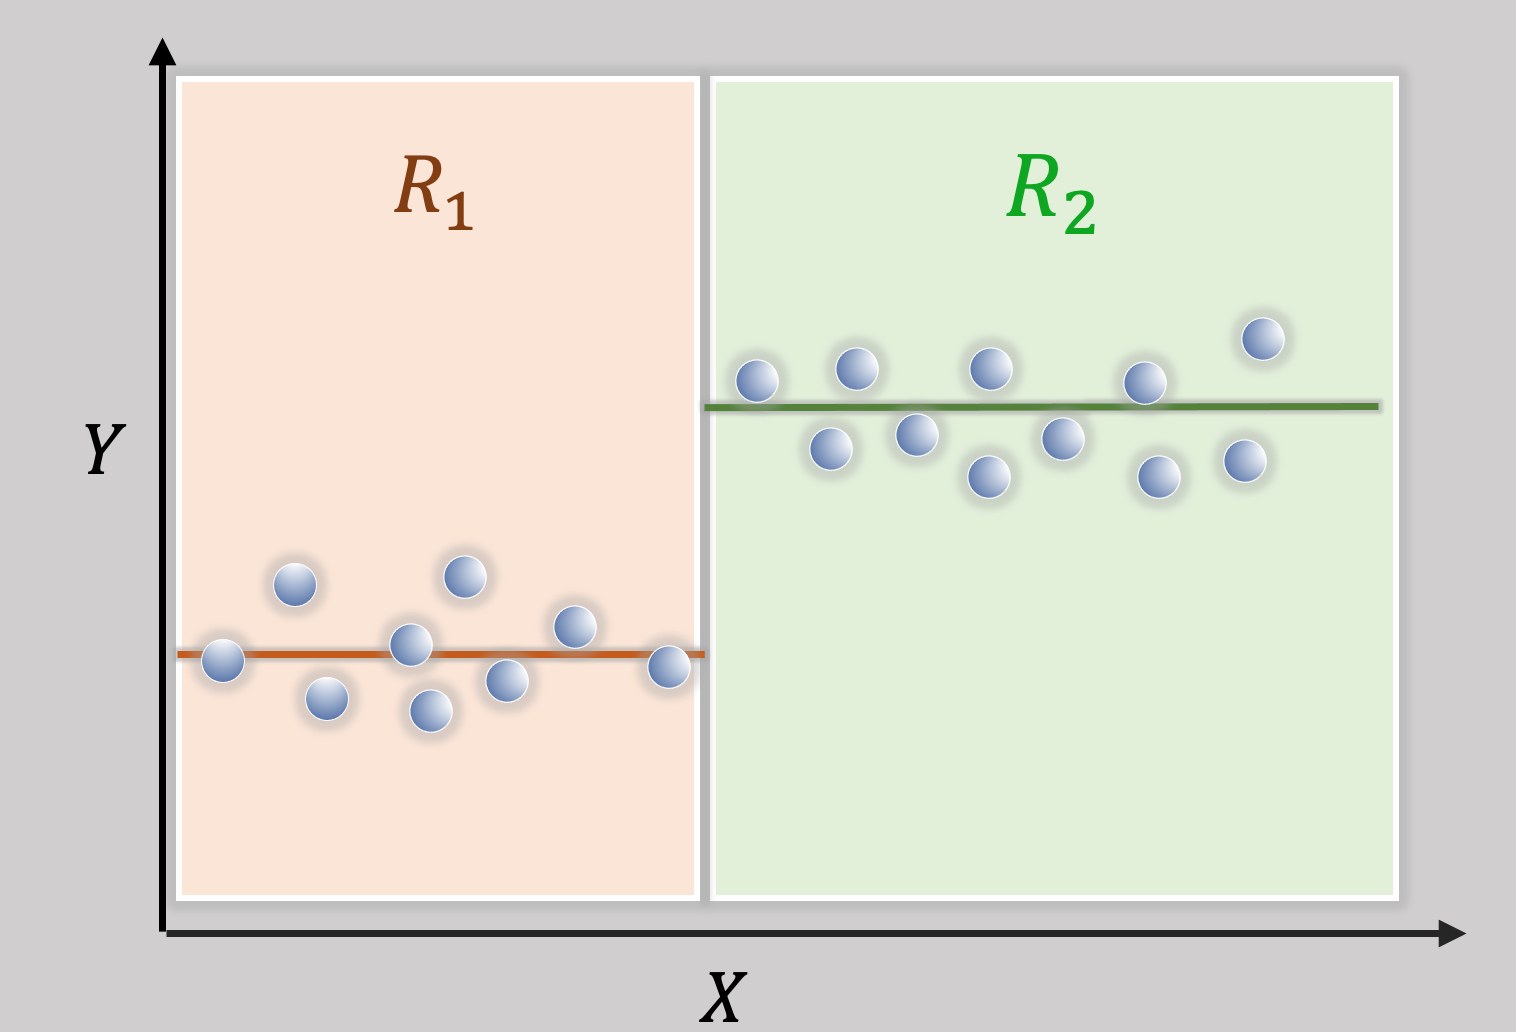
\includegraphics[scale=.3]{figs/RegressionTreeDiagram1.png}
\end{center}
}\\
\vspace{1in}
\end{frame}


\begin{frame}
\qBrd[4.1in]{babyblueeyes!50}{ $$\HLTW{ \displaystyle f(\bx )= \sum_{j=1}^{J} \HLTEQ[purple!40]{\HLTY{c_j }}\; \HLTEQ[babyblue!40]{ \Indicator{\bx \in \HLTEQ[rose!40]{\HLTY{R_j}}}} } $$}\\
\qBrd[4.1in]{babyblueeyes!60}{ $$\HLTW{ \displaystyle
\text{SSE}:= \sum_{i=1}^n \left(y_i -f(\bx_i) \right)^2
 } =   \DBX{\HLTW{ \displaystyle \sum_{j=1}^J  \sum_{i\in \HLTEQ[rose!40]{\HLTY{ R_j}}}^{}\left(y_i - \HLTY{ \widehat{c}_j} \right)^2  }}$$}\\
 
$$\DBX{ \HLTY{ \displaystyle  \widehat{c}_j}  =  \frac{1}{n_j} \sum_{i \in R_j } y_i    }$$
\end{frame}



\begin{frame}
\qBrd[4.5in]{babyblueeyes!50}{
\begin{center}
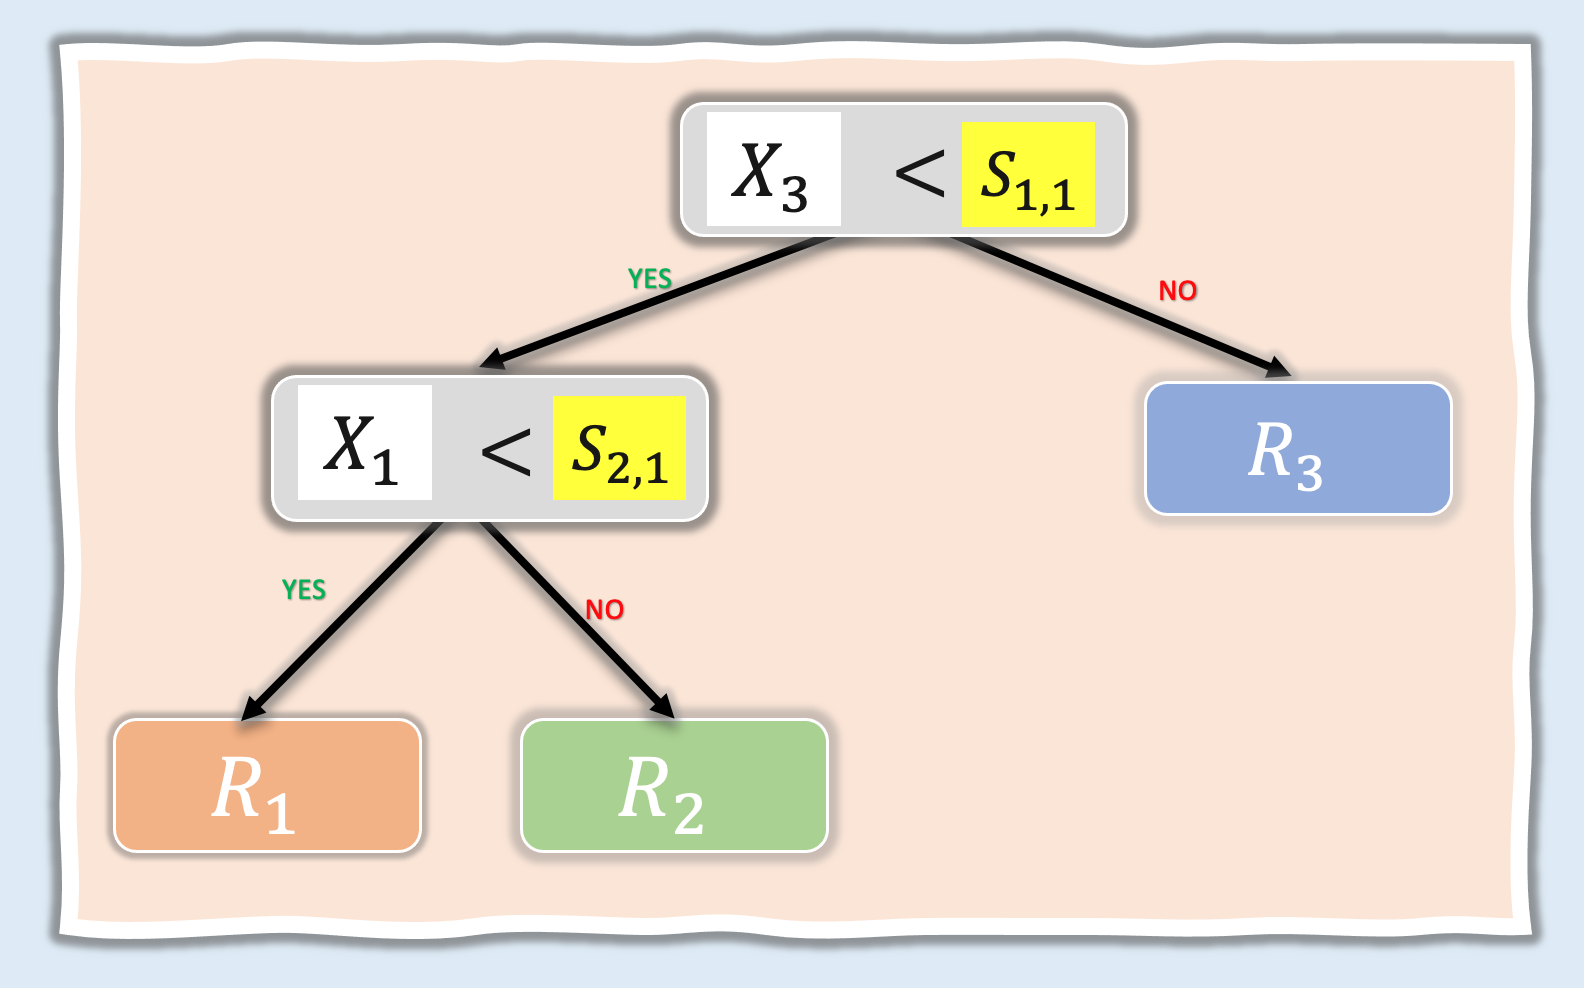
\includegraphics[scale=.32]{figs/RegressionTreeDiagram.png}
\end{center}
%\vspace{.1in}
\begin{enumerate}
\qBrd[4in]{airforceblue!50}{
\item[\sqBullet{bluebell}] How do we decide which varibale to select while creating the binary split? i.e. which one among  $\HLTW{\{X_1, \ldots X_p\}}$
}
\qBrd[4in]{babyblue!50}{
\item[\sqBullet{babyblue}]  How do we select the cut off $\HLTY{S}$?
}
\end{enumerate}
}\\
\vspace{.2in}

\end{frame}






\begin{frame}
\vspace{-.2in}
\qBrd[4.5in]{babyblueeyes!50}{
\begin{center}
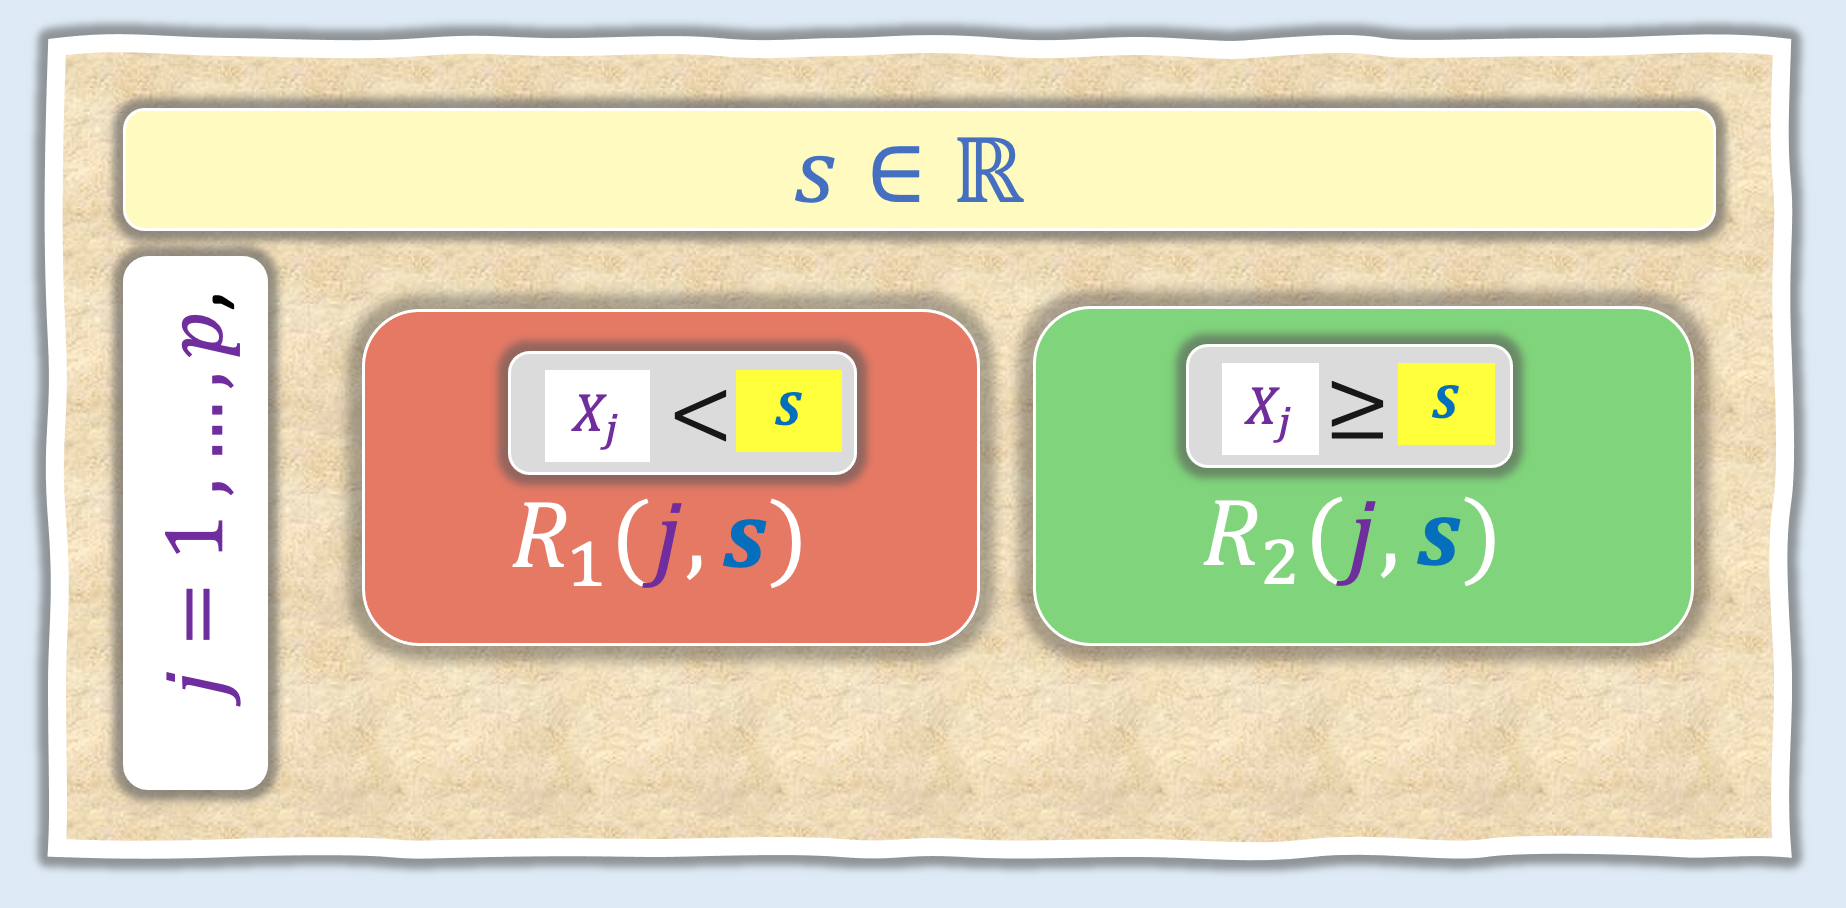
\includegraphics[scale=.3]{figs/R1_R2.png}
\end{center}
\vspace{-.15in}
}\\
\vspace{-.18in}
\begin{center}
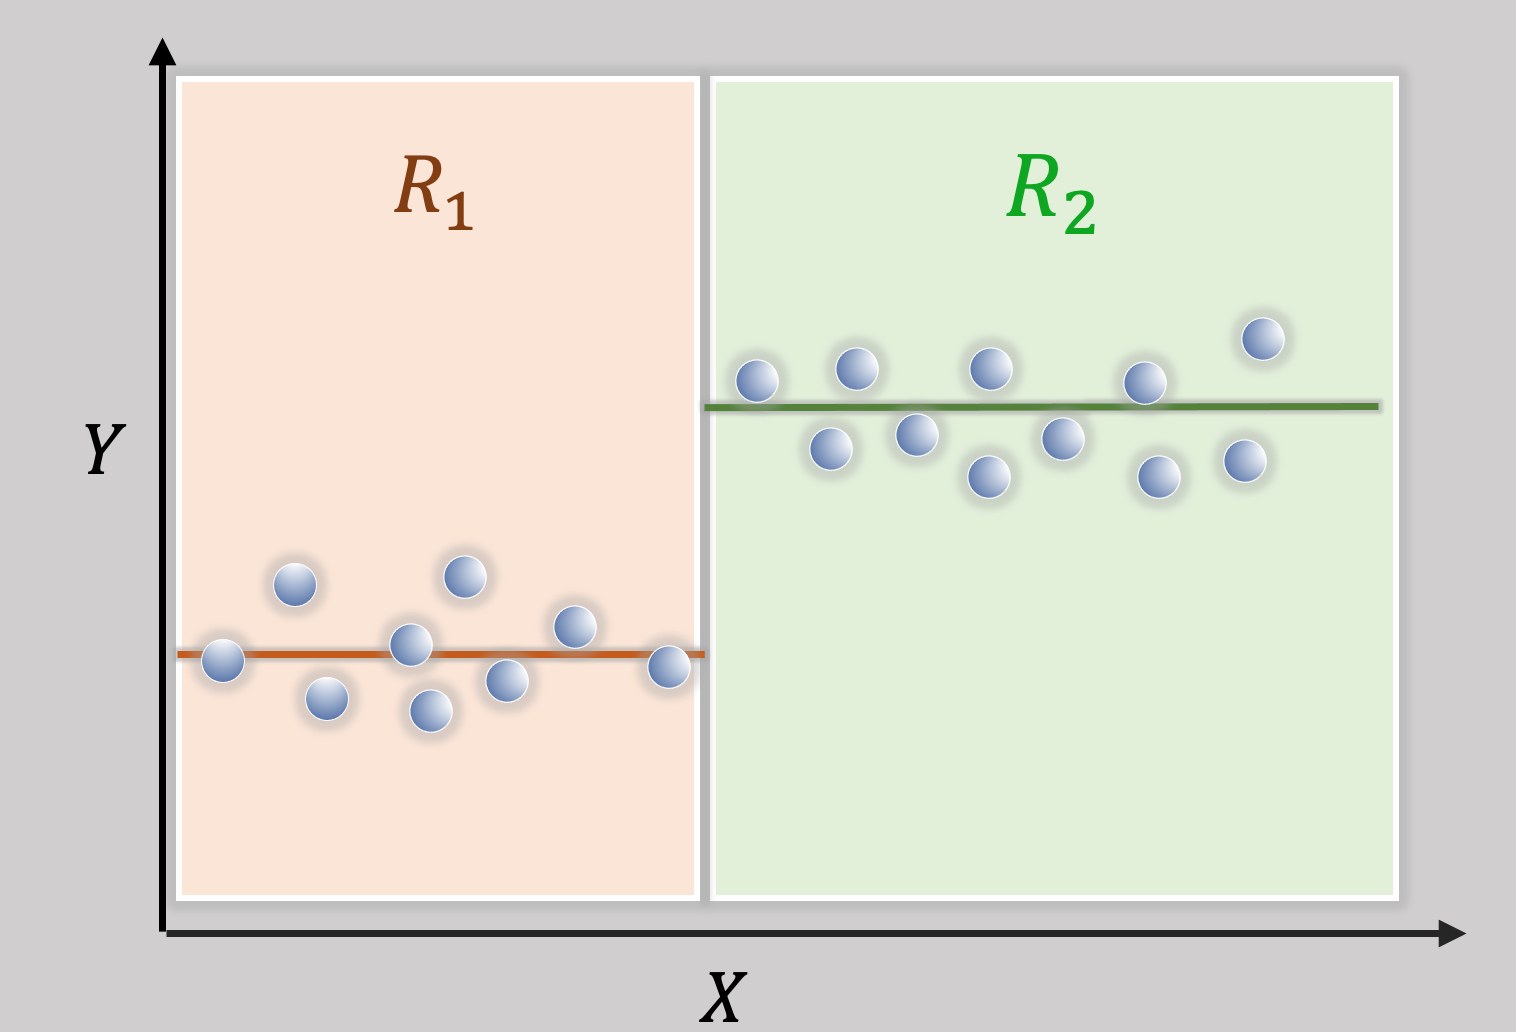
\includegraphics[scale=.22]{figs/RegressionTreeDiagram1.png}
\end{center}
\vspace{-.15in}
\end{frame}



\begin{frame}
\qBrd[4.7in]{babyblueeyes!50}{
\begin{center}
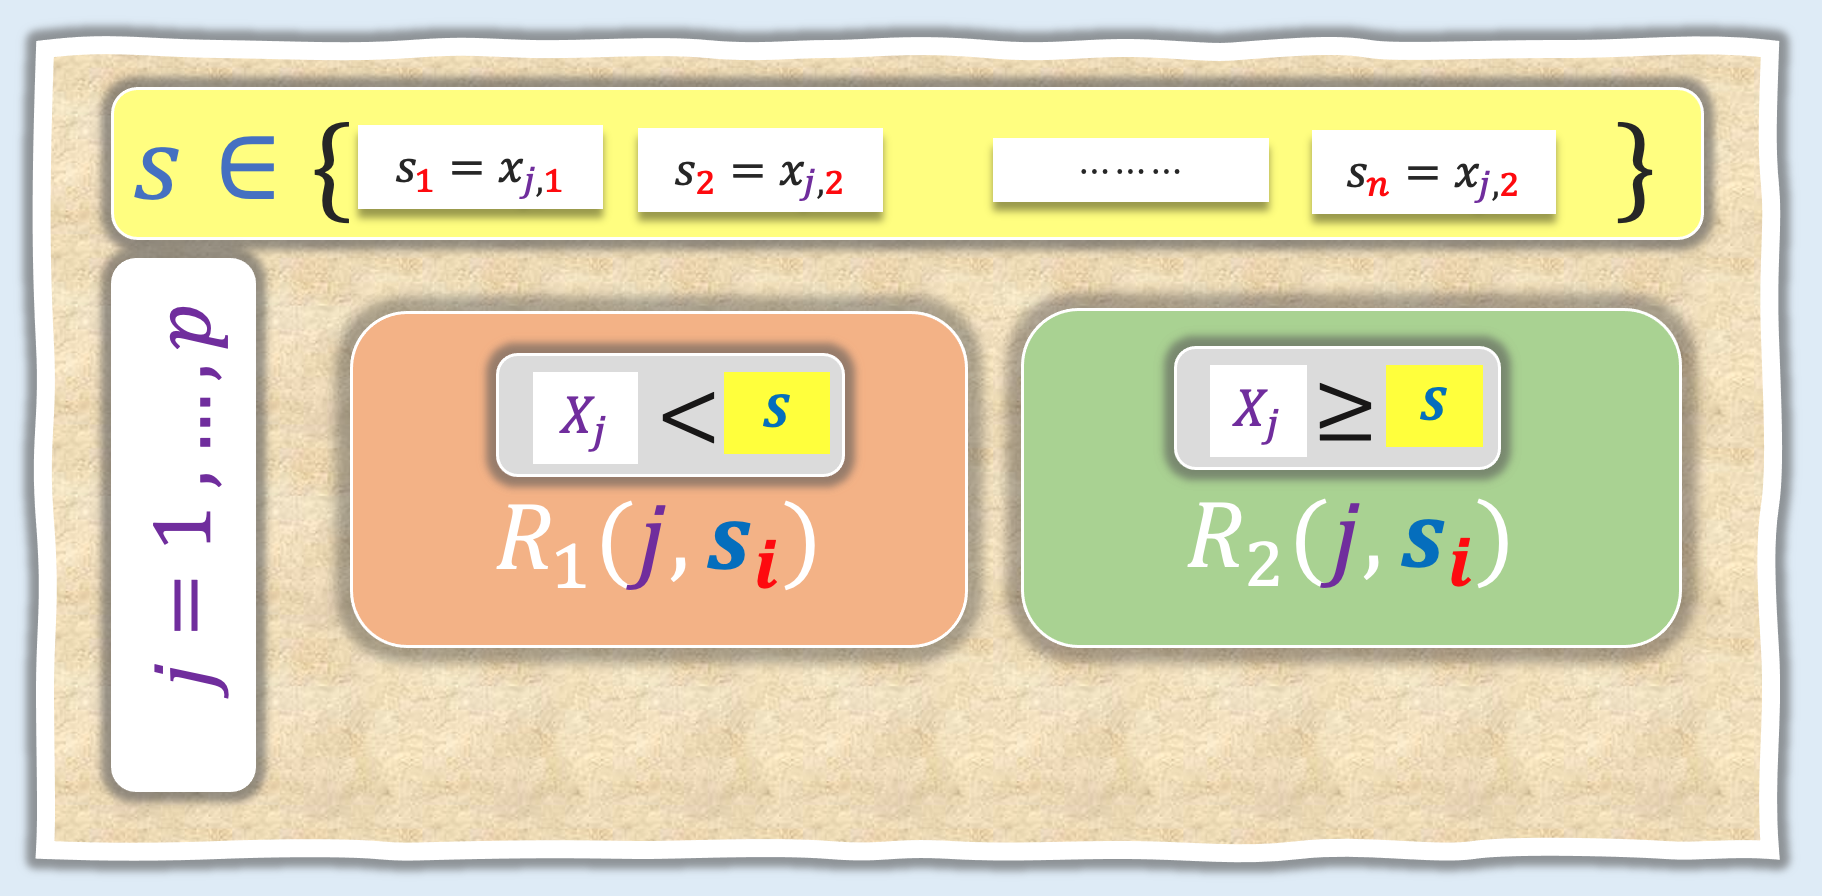
\includegraphics[scale=.35]{figs/R1_R2_s.png}
\end{center}
%\vspace{.1in}
}\\
\qBrd[4.7in]{airforceblue!50}{$$\HLTW{ \text{C}(j, s_i)}:=  {\HLTW{ \displaystyle  \sum_{\HLTEQ[rose!40]{i\in \HLTY{ R_1(j, s_i)}}}^{}\left(y_i - \HLTY{ \widehat{y}_{_{R_1}}} \right)^2  } + \HLTW{ \displaystyle  \sum_{ \HLTEQ[rose!40]{i\in \HLTY{ R_2(j, s_i)}}}^{}\left(y_i - \HLTY{ \widehat{y}_{_{R_2}}} \right)^2  }}$$
}

\end{frame}






\begin{frame}
\qBrd[4.6in]{babyblueeyes!50}{
\begin{center}
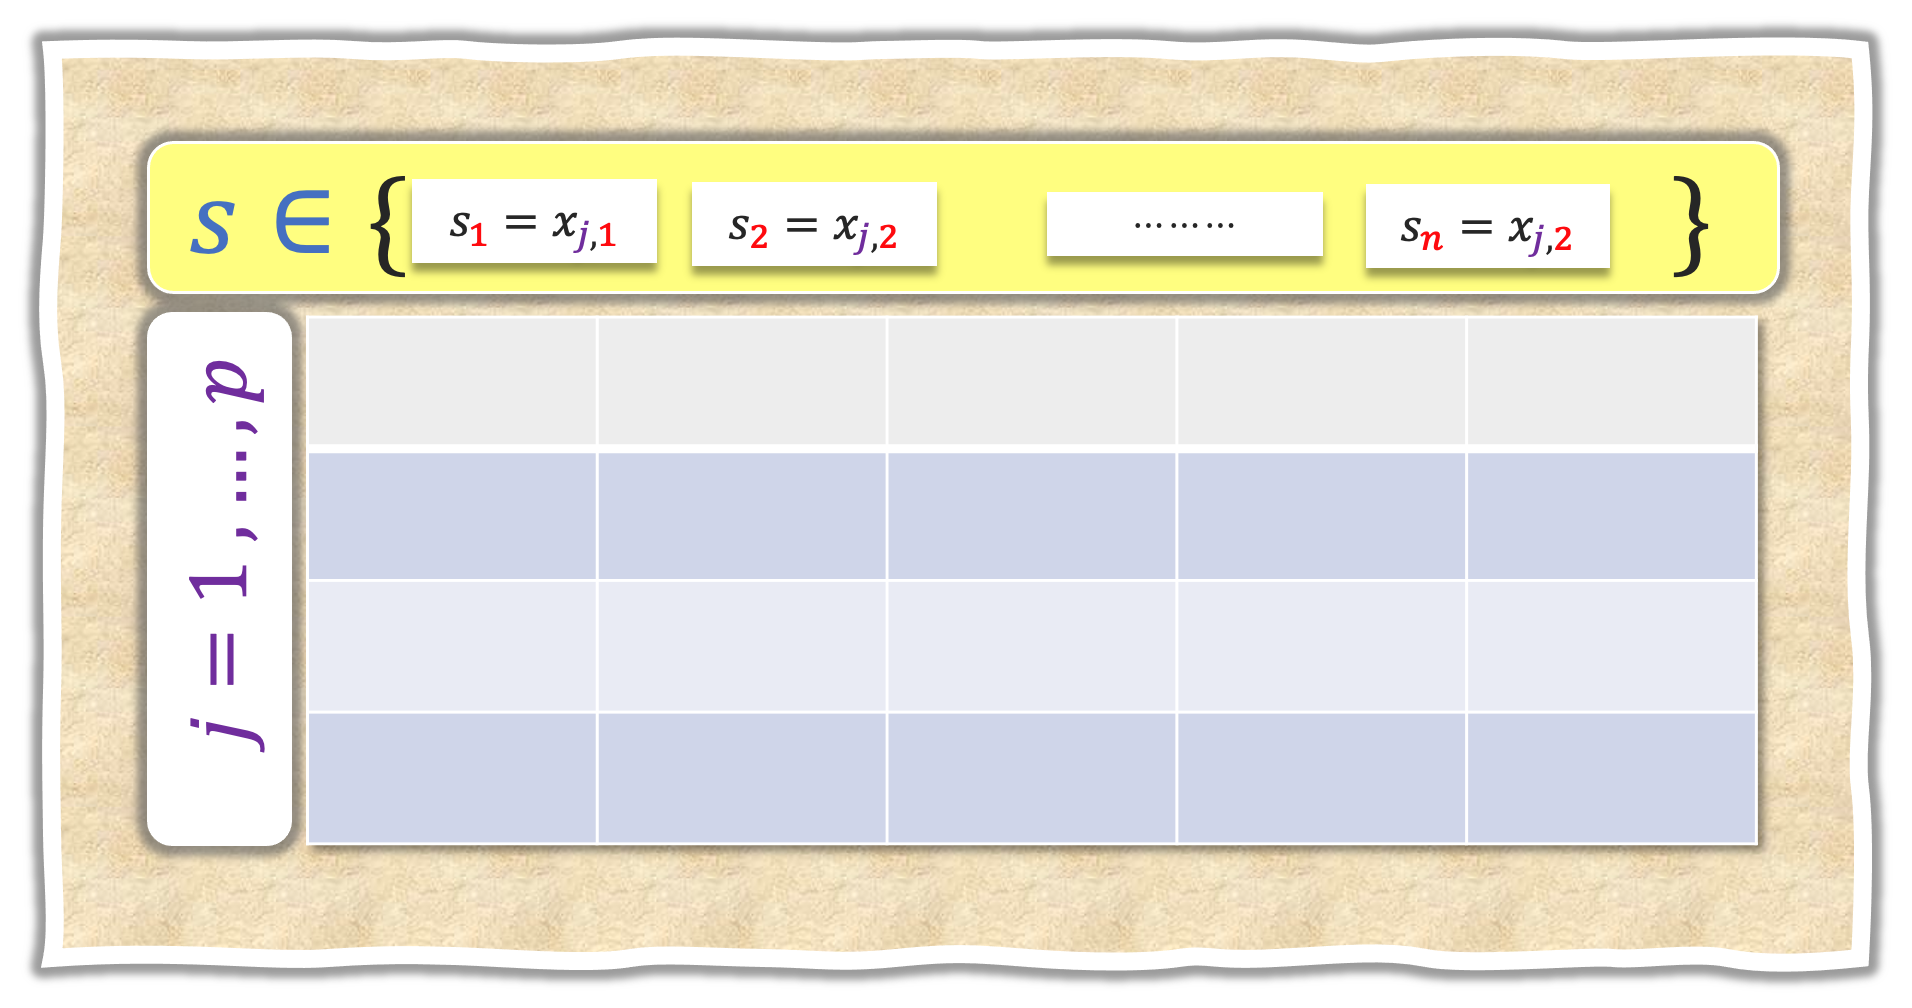
\includegraphics[scale=.35]{figs/R1_R2_table.png}
\end{center}
%\vspace{.1in}
%\begin{enumerate}
%%\qBrd[4in]{airforceblue!50}{
%%\item[\sqBullet{bluebell}] A
%%}
%%\qBrd[4in]{babyblue!50}{
%%\item[\sqBullet{babyblue}]  A
%%}
%\end{enumerate}
}\\
\vspace{.2in}

\end{frame}




\begin{frame}
\qBrd[4.7in]{babyblueeyes!50}{
\begin{center}
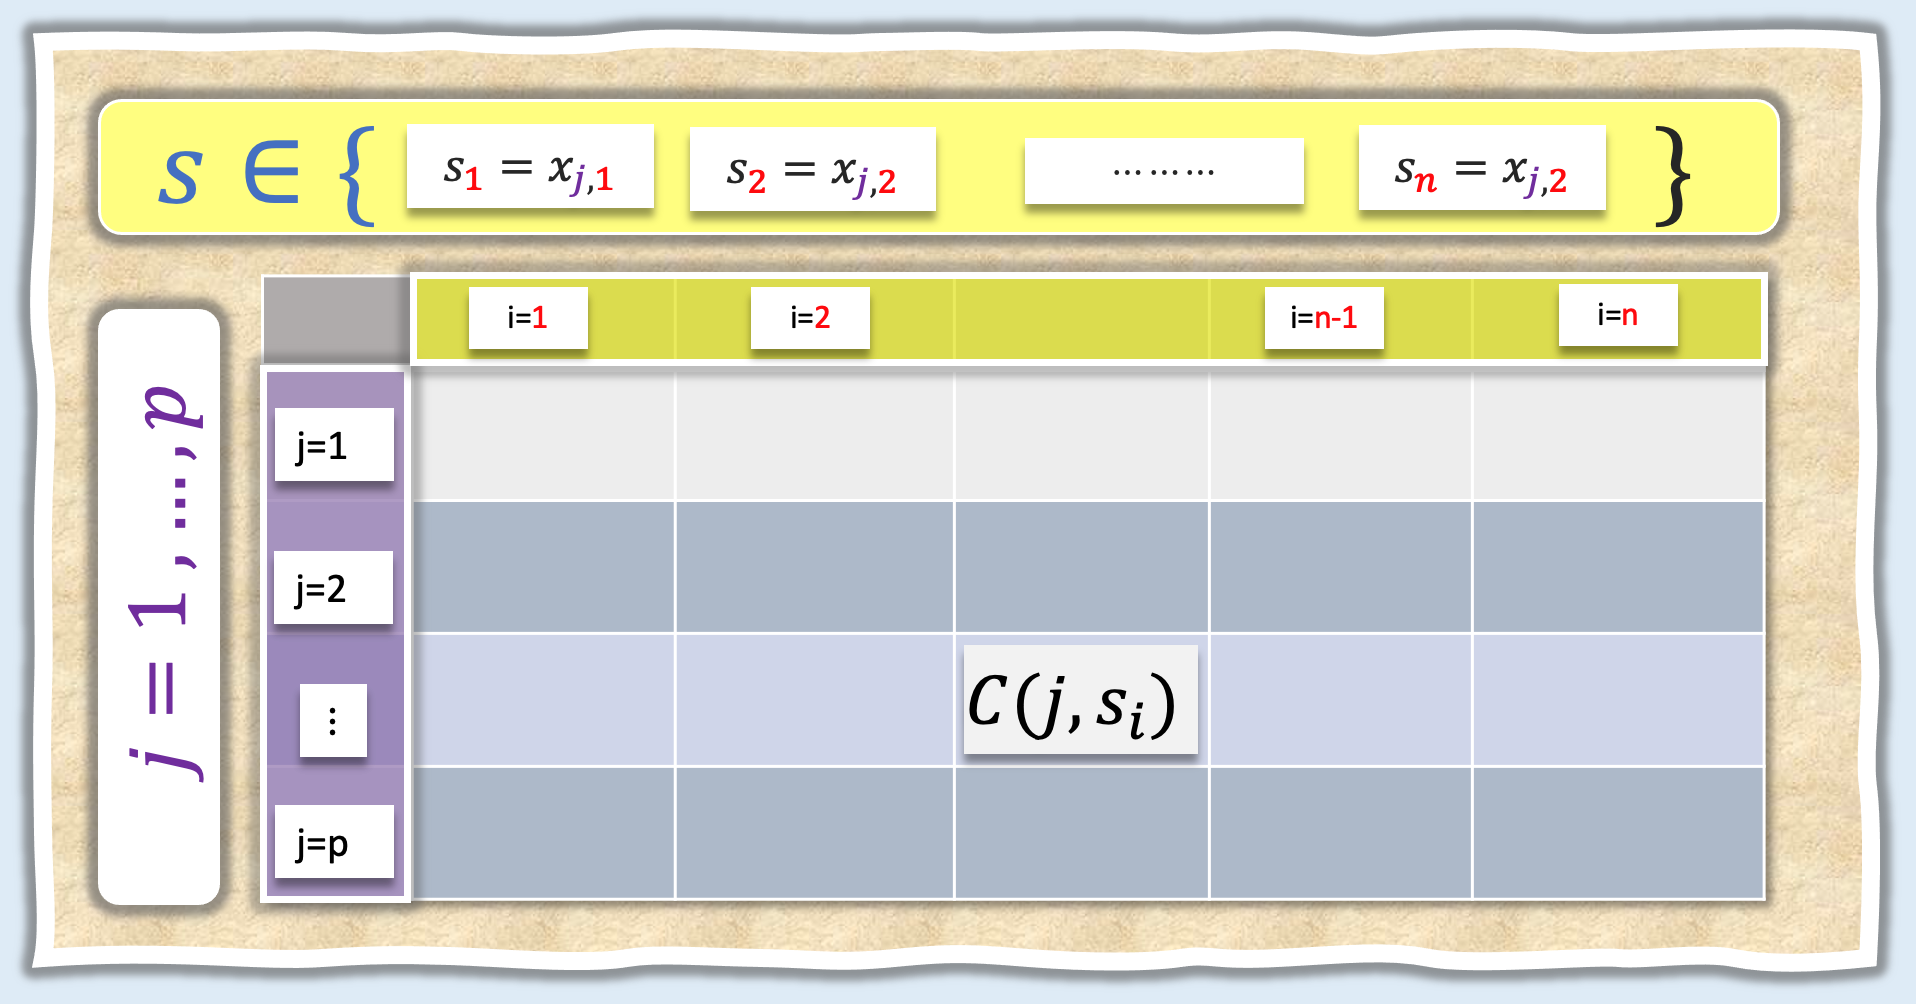
\includegraphics[scale=.35]{figs/R1_R2_table1.png}
\end{center}
%\vspace{.1in}
%\begin{enumerate}
%\qBrd[4in]{airforceblue!50}{
%\item[\sqBullet{bluebell}] A
%}
%\qBrd[4in]{babyblue!50}{
%\item[\sqBullet{babyblue}]  A
%}
%\end{enumerate}
}\\
\vspace{.8in}

\end{frame}


\subsection{An Example}

\begin{frame}
\qBrd[4.7in]{babyblueeyes!50}{
\begin{center}
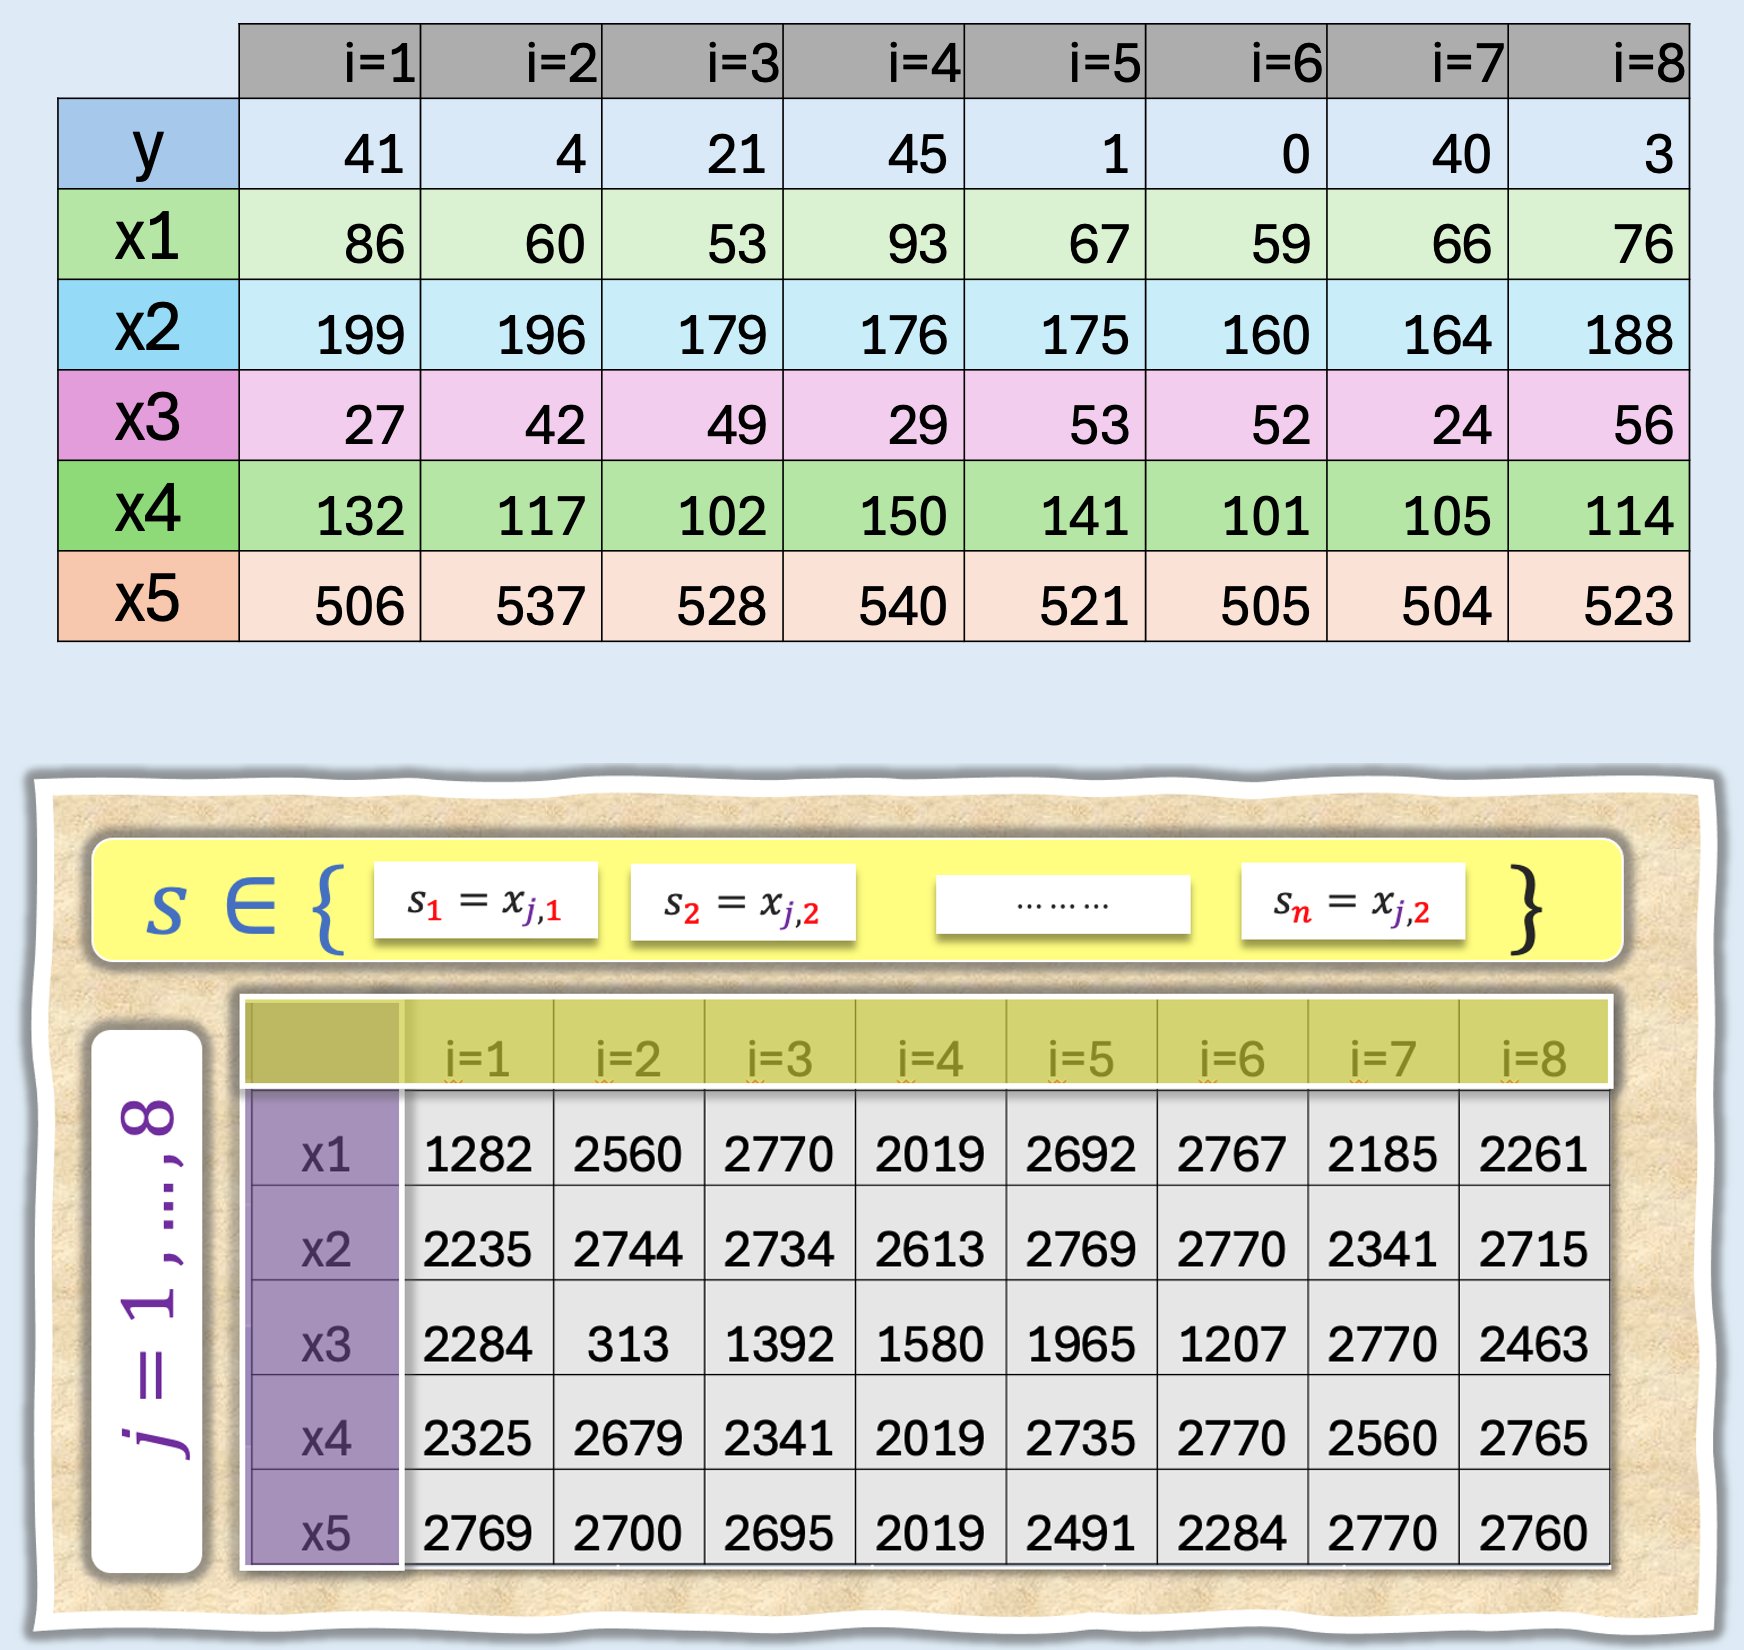
\includegraphics[scale=.28]{figs/R1_R2_table_Example.png}
\end{center}
%\vspace{.1in}
%\begin{enumerate}
%\qBrd[4in]{airforceblue!50}{
%\item[\sqBullet{bluebell}] A
%}
%\qBrd[4in]{babyblue!50}{
%\item[\sqBullet{babyblue}]  A
%}
%\end{enumerate}
}\\
\vspace{.8in}

\end{frame}



\begin{frame}
\qBrd[4.7in]{babyblueeyes!50}{
\begin{center}
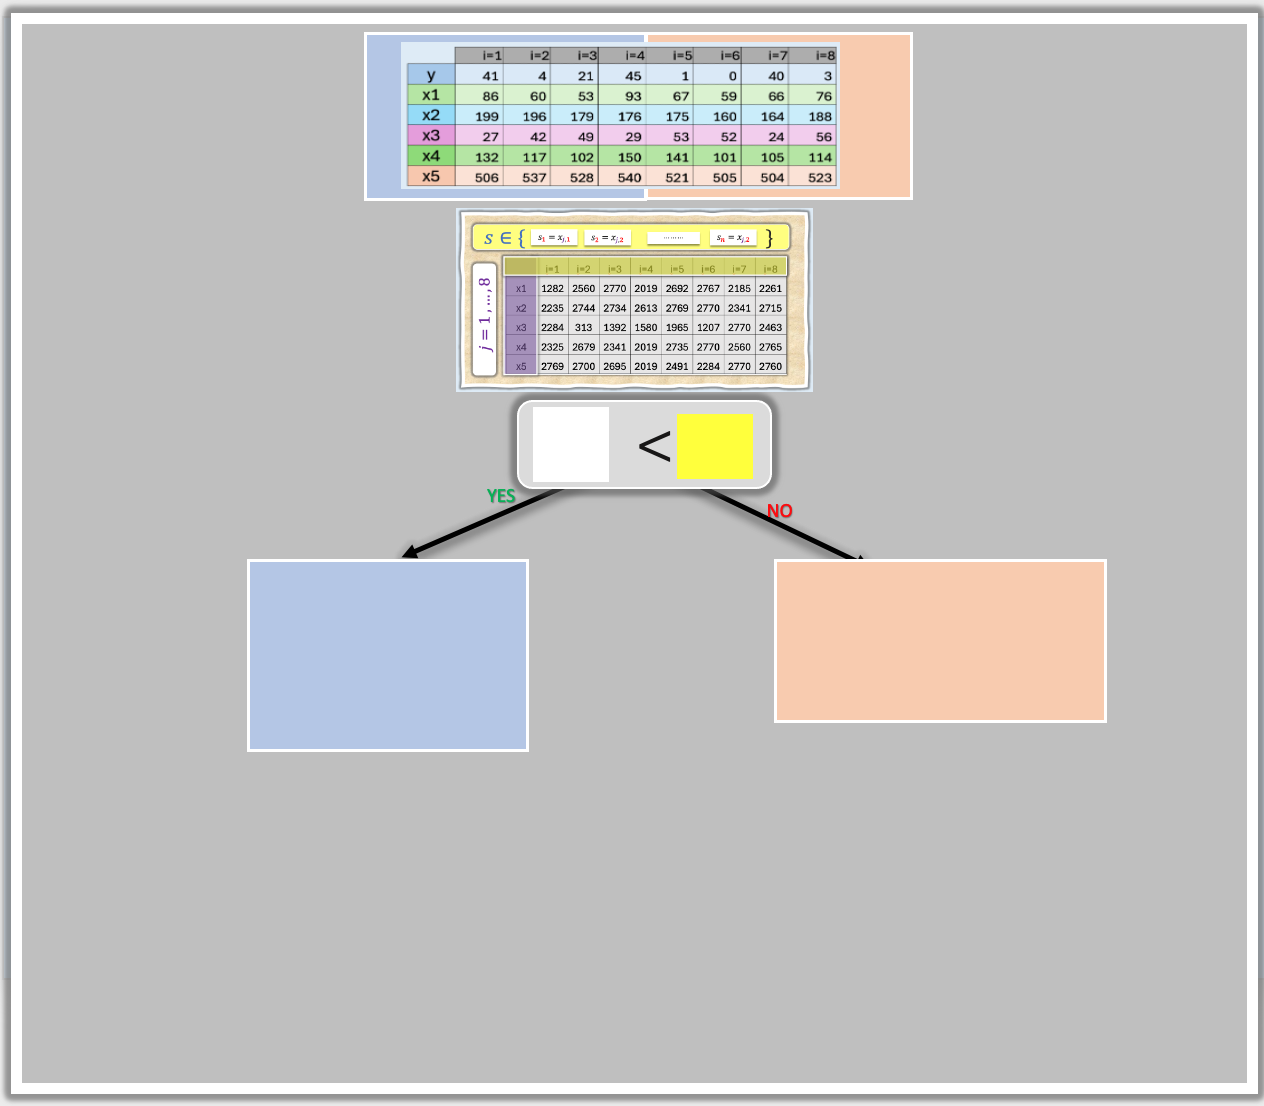
\includegraphics[scale=.4]{figs/TREE_CONSTRUCTION0.png}
\end{center}
}\\
\vspace{.2in}

\end{frame}




\begin{frame}
\qBrd[4.7in]{babyblueeyes!50}{
\begin{center}
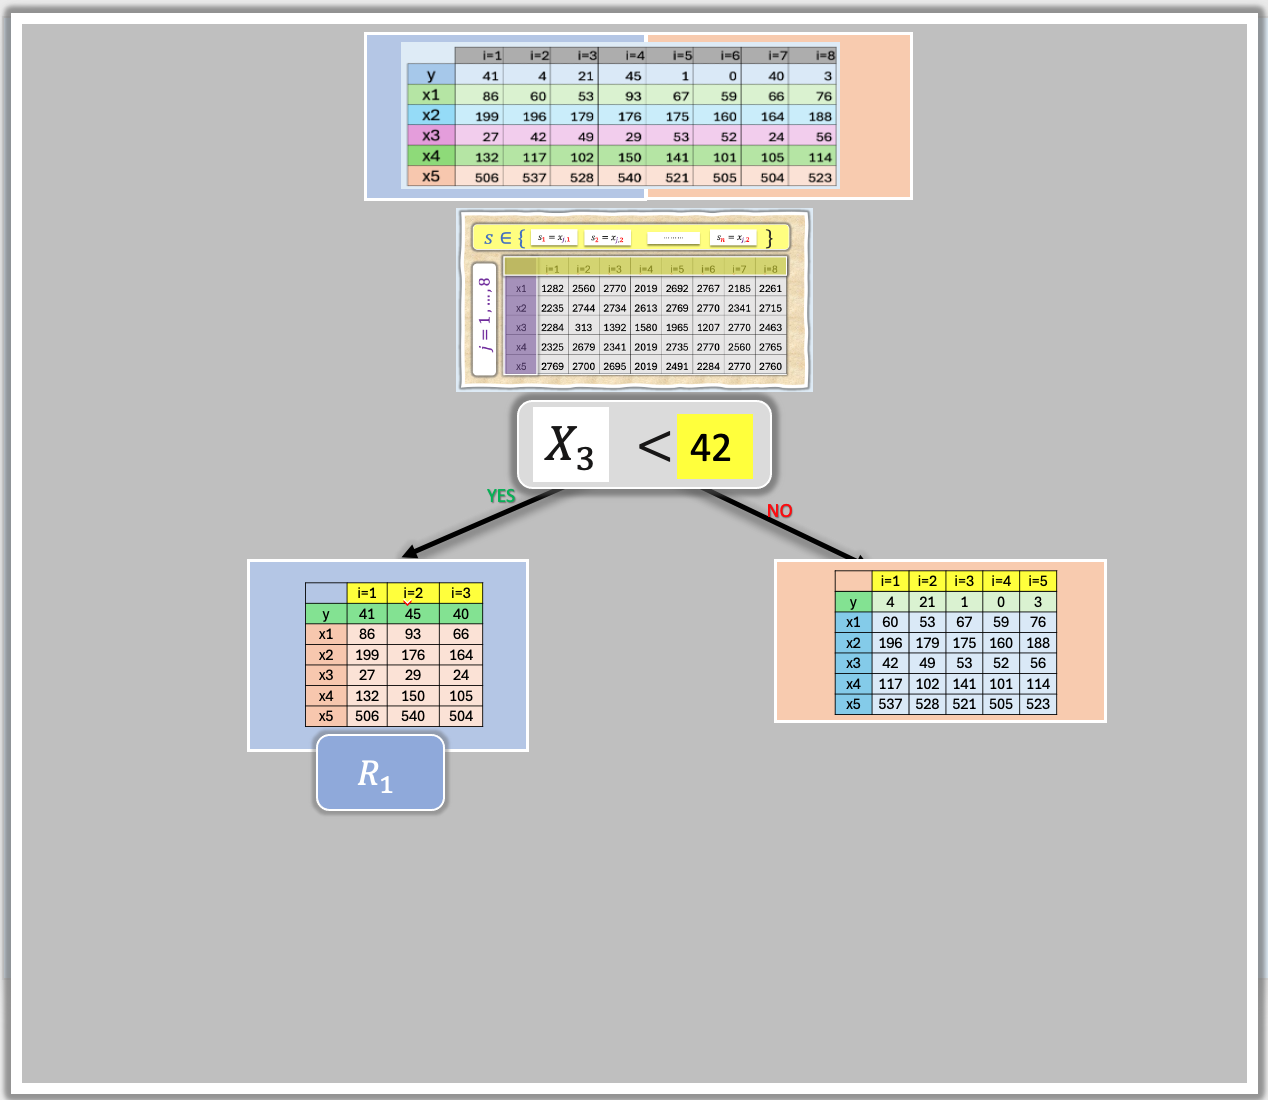
\includegraphics[scale=.4]{figs/TREE_CONSTRUCTION01.png}
\end{center}
}\\
\vspace{.2in}

\end{frame}


\begin{frame}
\qBrd[4.7in]{babyblueeyes!50}{
\begin{center}
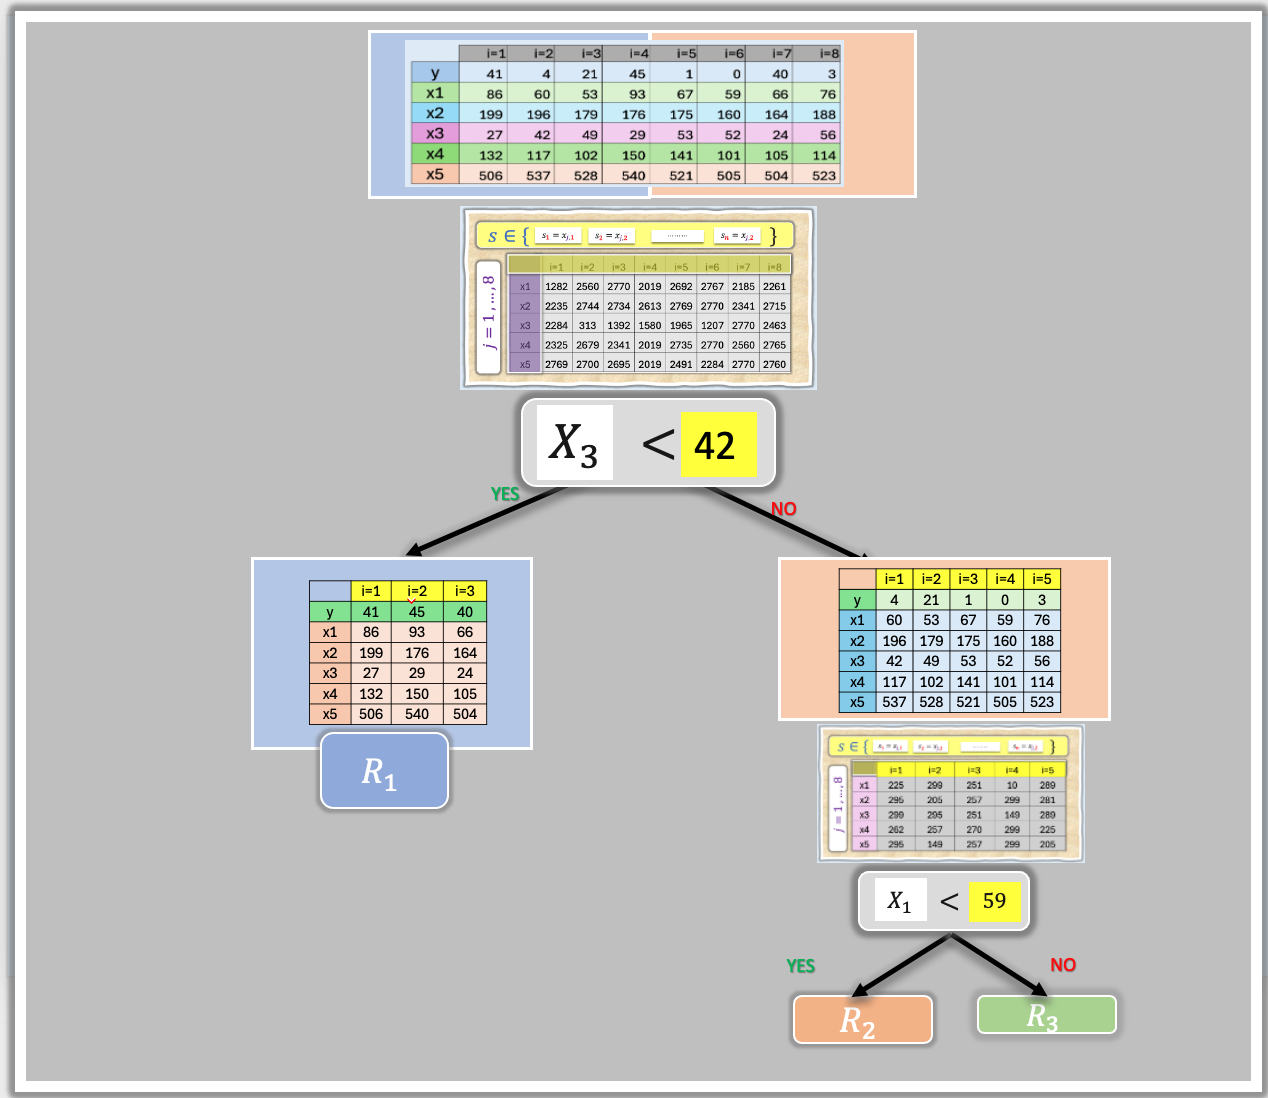
\includegraphics[scale=.4]{figs/TREE_CONSTRUCTION.png}
\end{center}
%\vspace{.1in}
%\begin{enumerate}
%\qBrd[4in]{airforceblue!50}{
%\item[\sqBullet{bluebell}] A
%}
%\qBrd[4in]{babyblue!50}{
%\item[\sqBullet{babyblue}]  A
%}
%\end{enumerate}
}\\
\vspace{.2in}

\end{frame}





{ \setbeamercolor{background canvas}{bg=}
\includepdf[pages={81-83}, scale=1]{STAT380-Unit3.pdf}
}







\TransitionFrame[antiquebrass]{\Large Tree, Subtree,  and Tree Pruning }
%





\TransitionFrame[olive]{\Large Subtree }
%




\begin{frame}
\qBrd[4.7in]{babyblueeyes!50}{
\vspace{-.2in}
\begin{center}
\qBrd[.3in]{babyblueeyes}{$\;\HLTW{T_0}$}
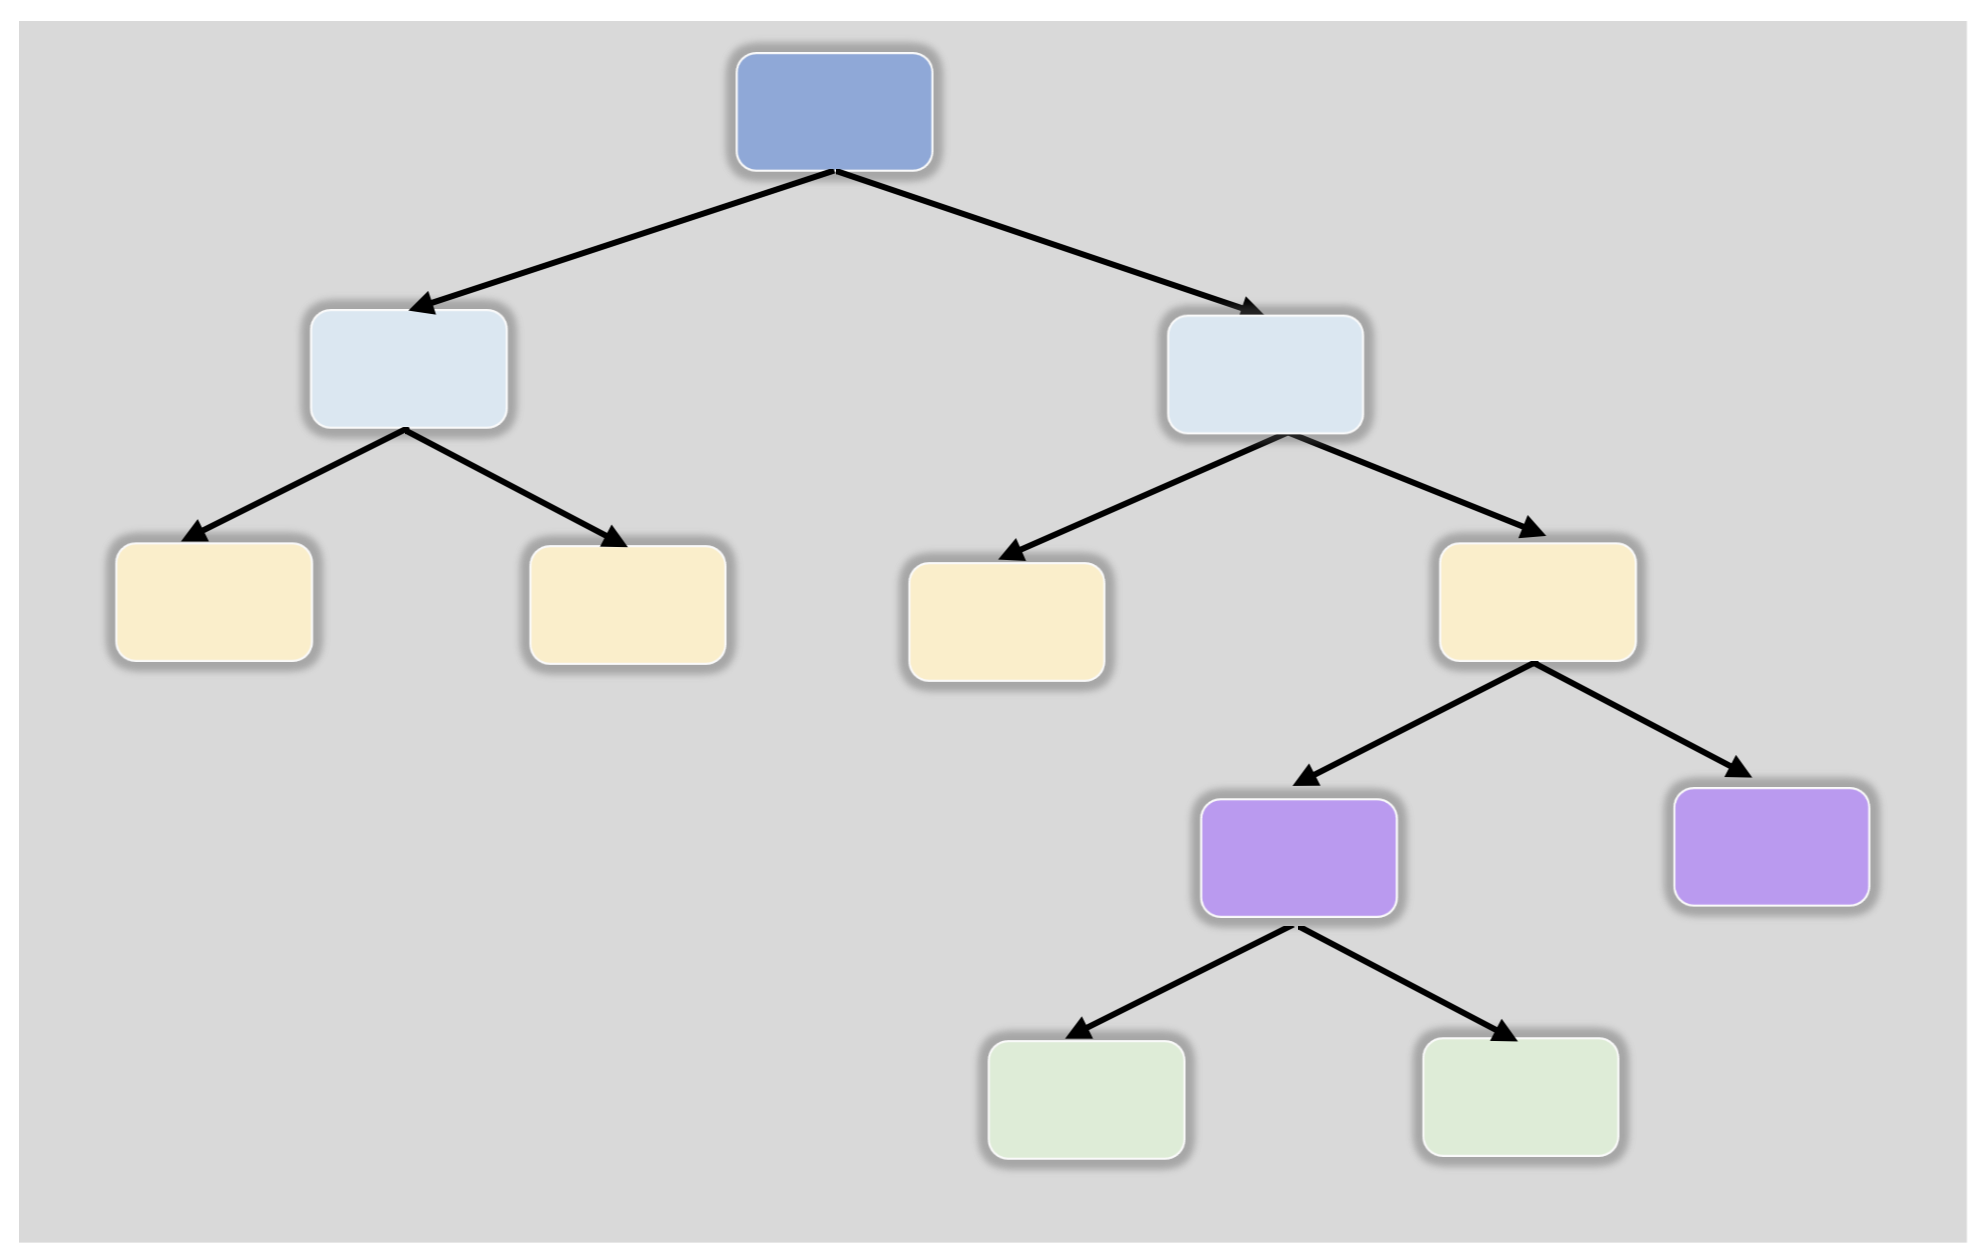
\includegraphics[scale=.32]{figs/T0.png}
\end{center}
}\\
\end{frame}



\begin{frame}
\qBrd[4.7in]{babyblueeyes!50}{
\begin{center}
$\Col{
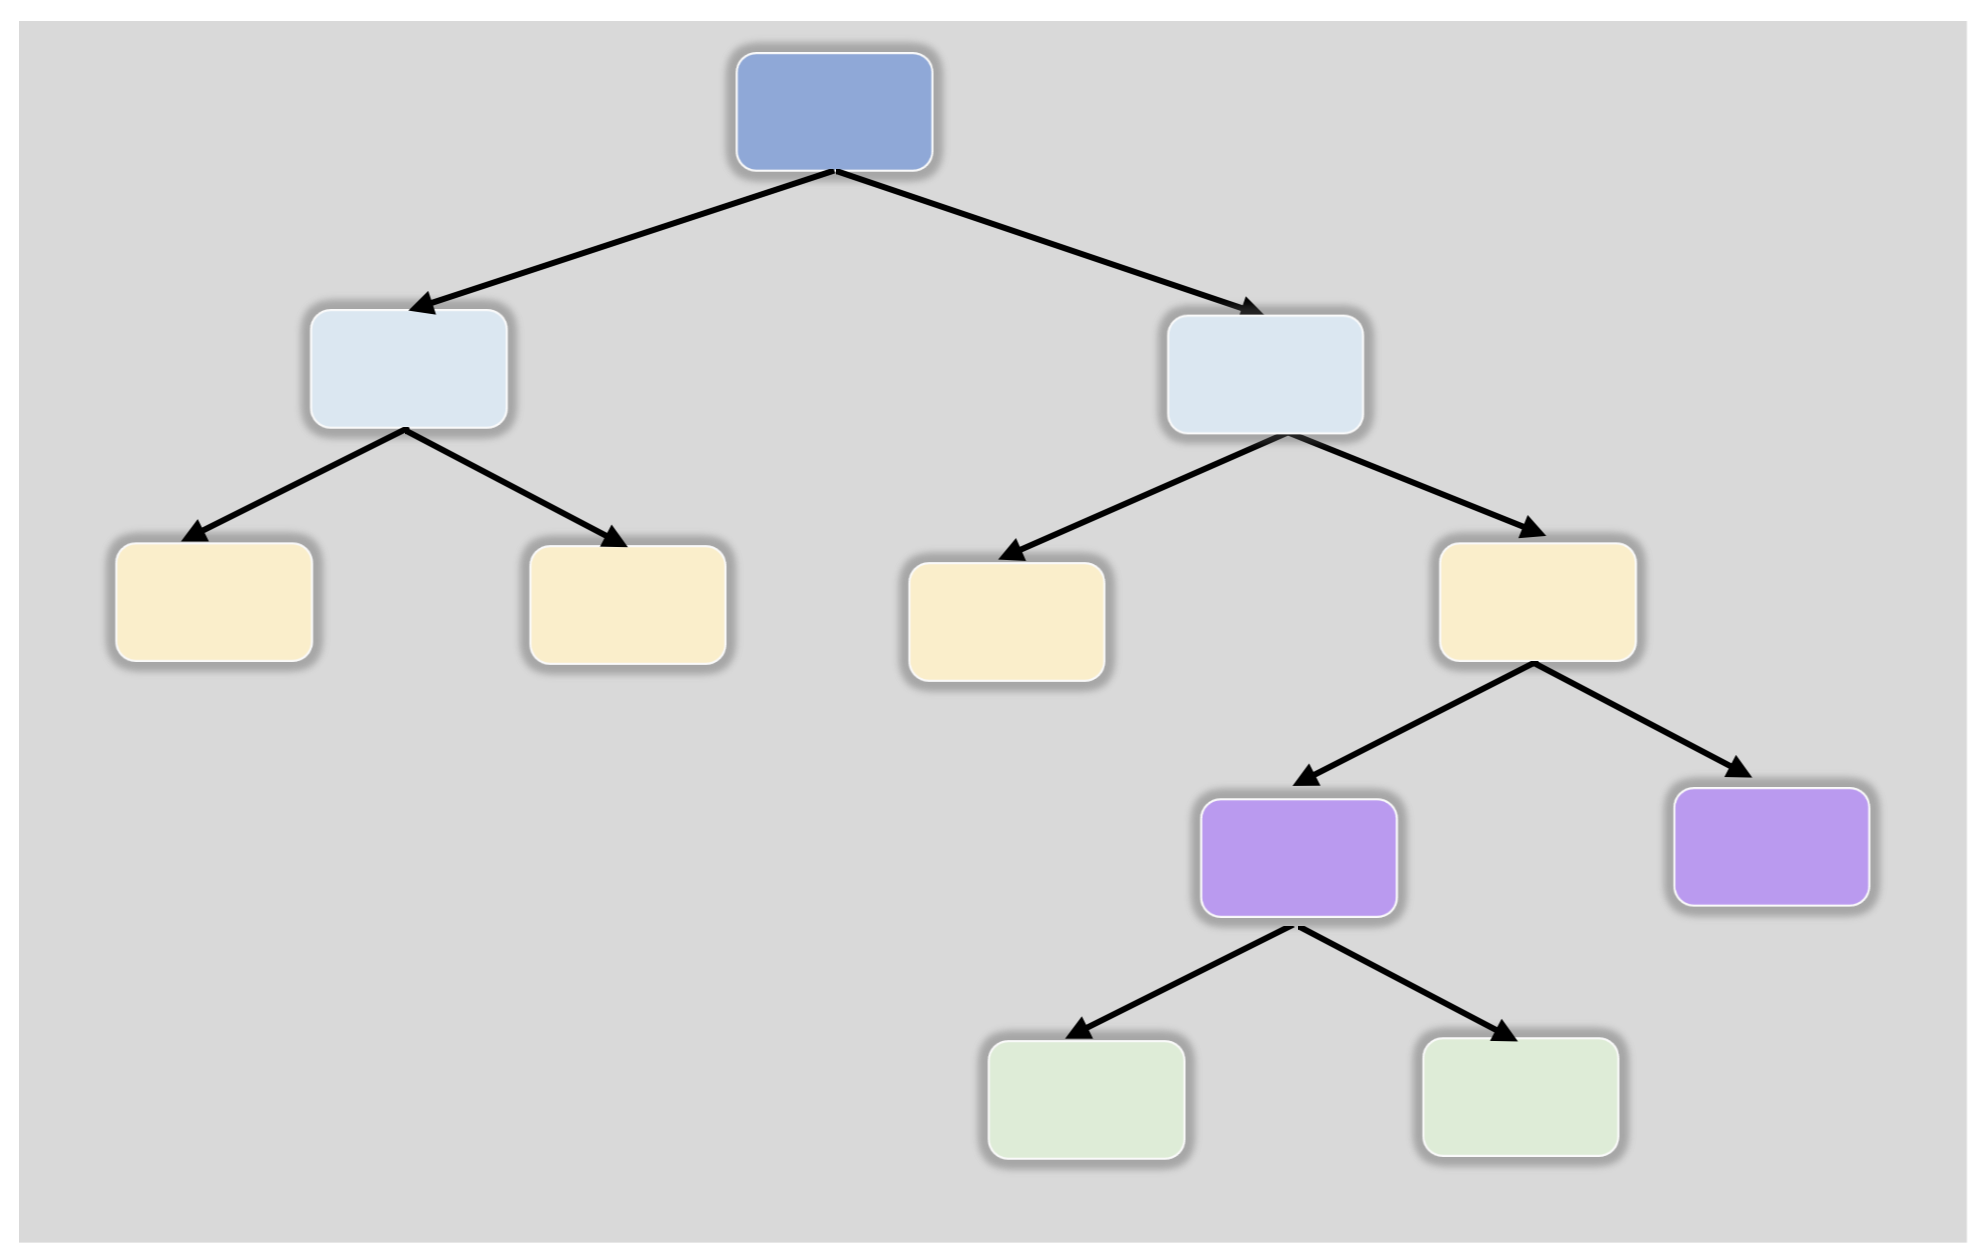
\includegraphics[scale=.15]{figs/T0.png},
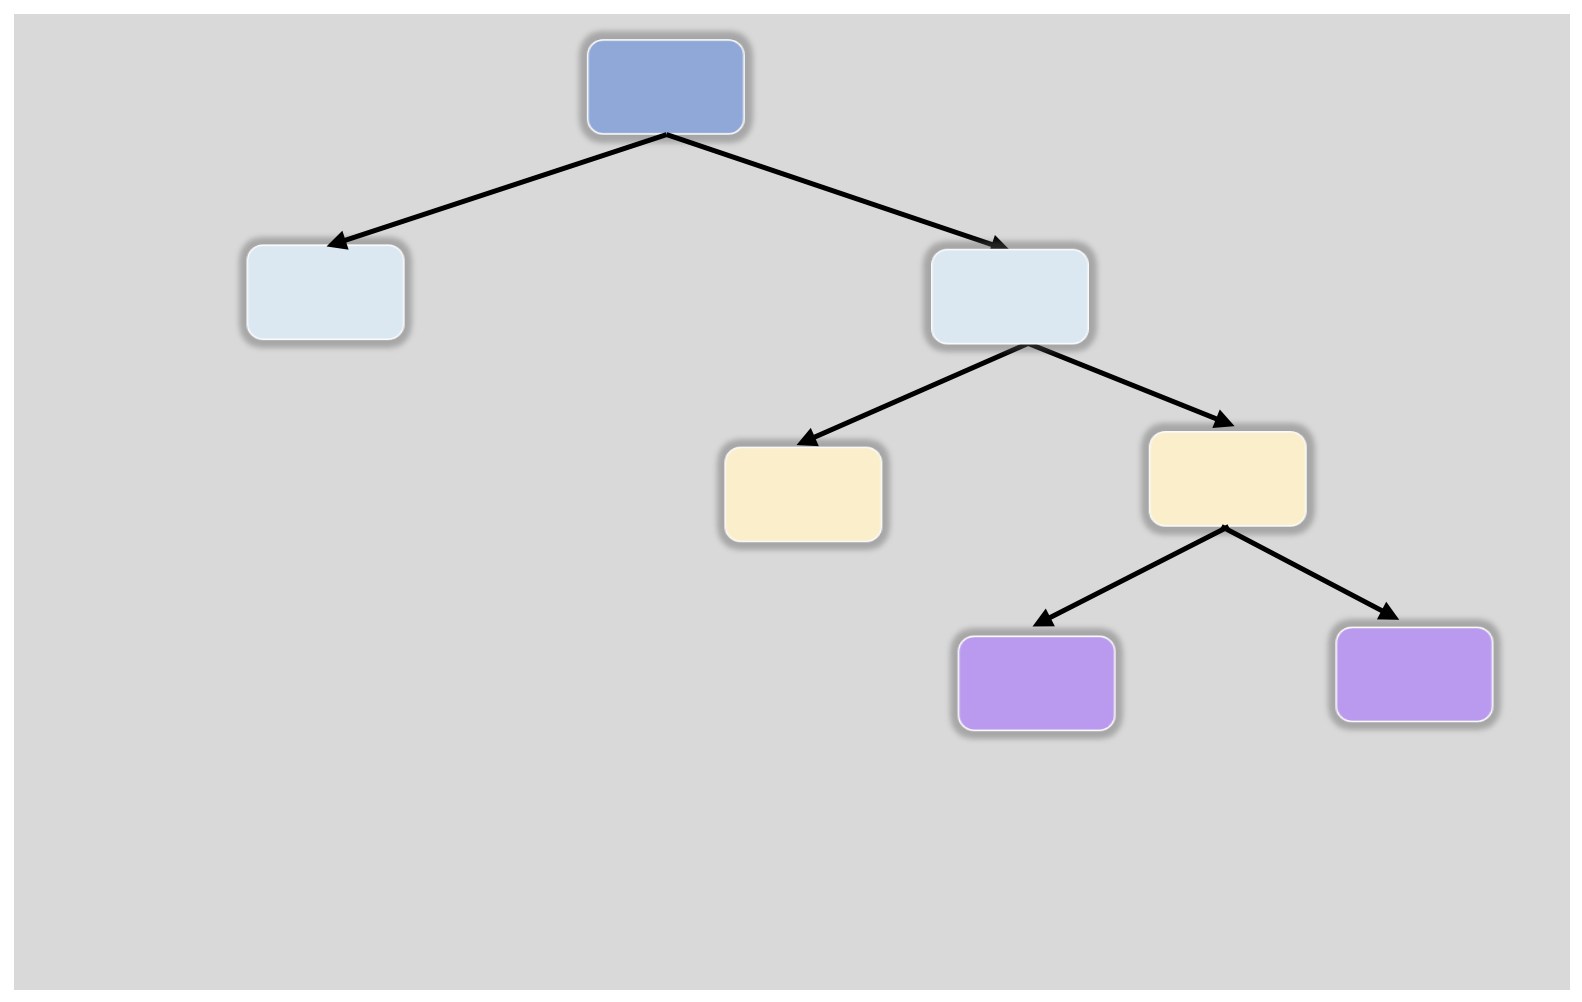
\includegraphics[scale=.28]{figs/T1.png}}$
\end{center}
}\\
\end{frame}






\begin{frame}
\qBrd[4.7in]{babyblueeyes!50}{
\begin{center}
$\Col{
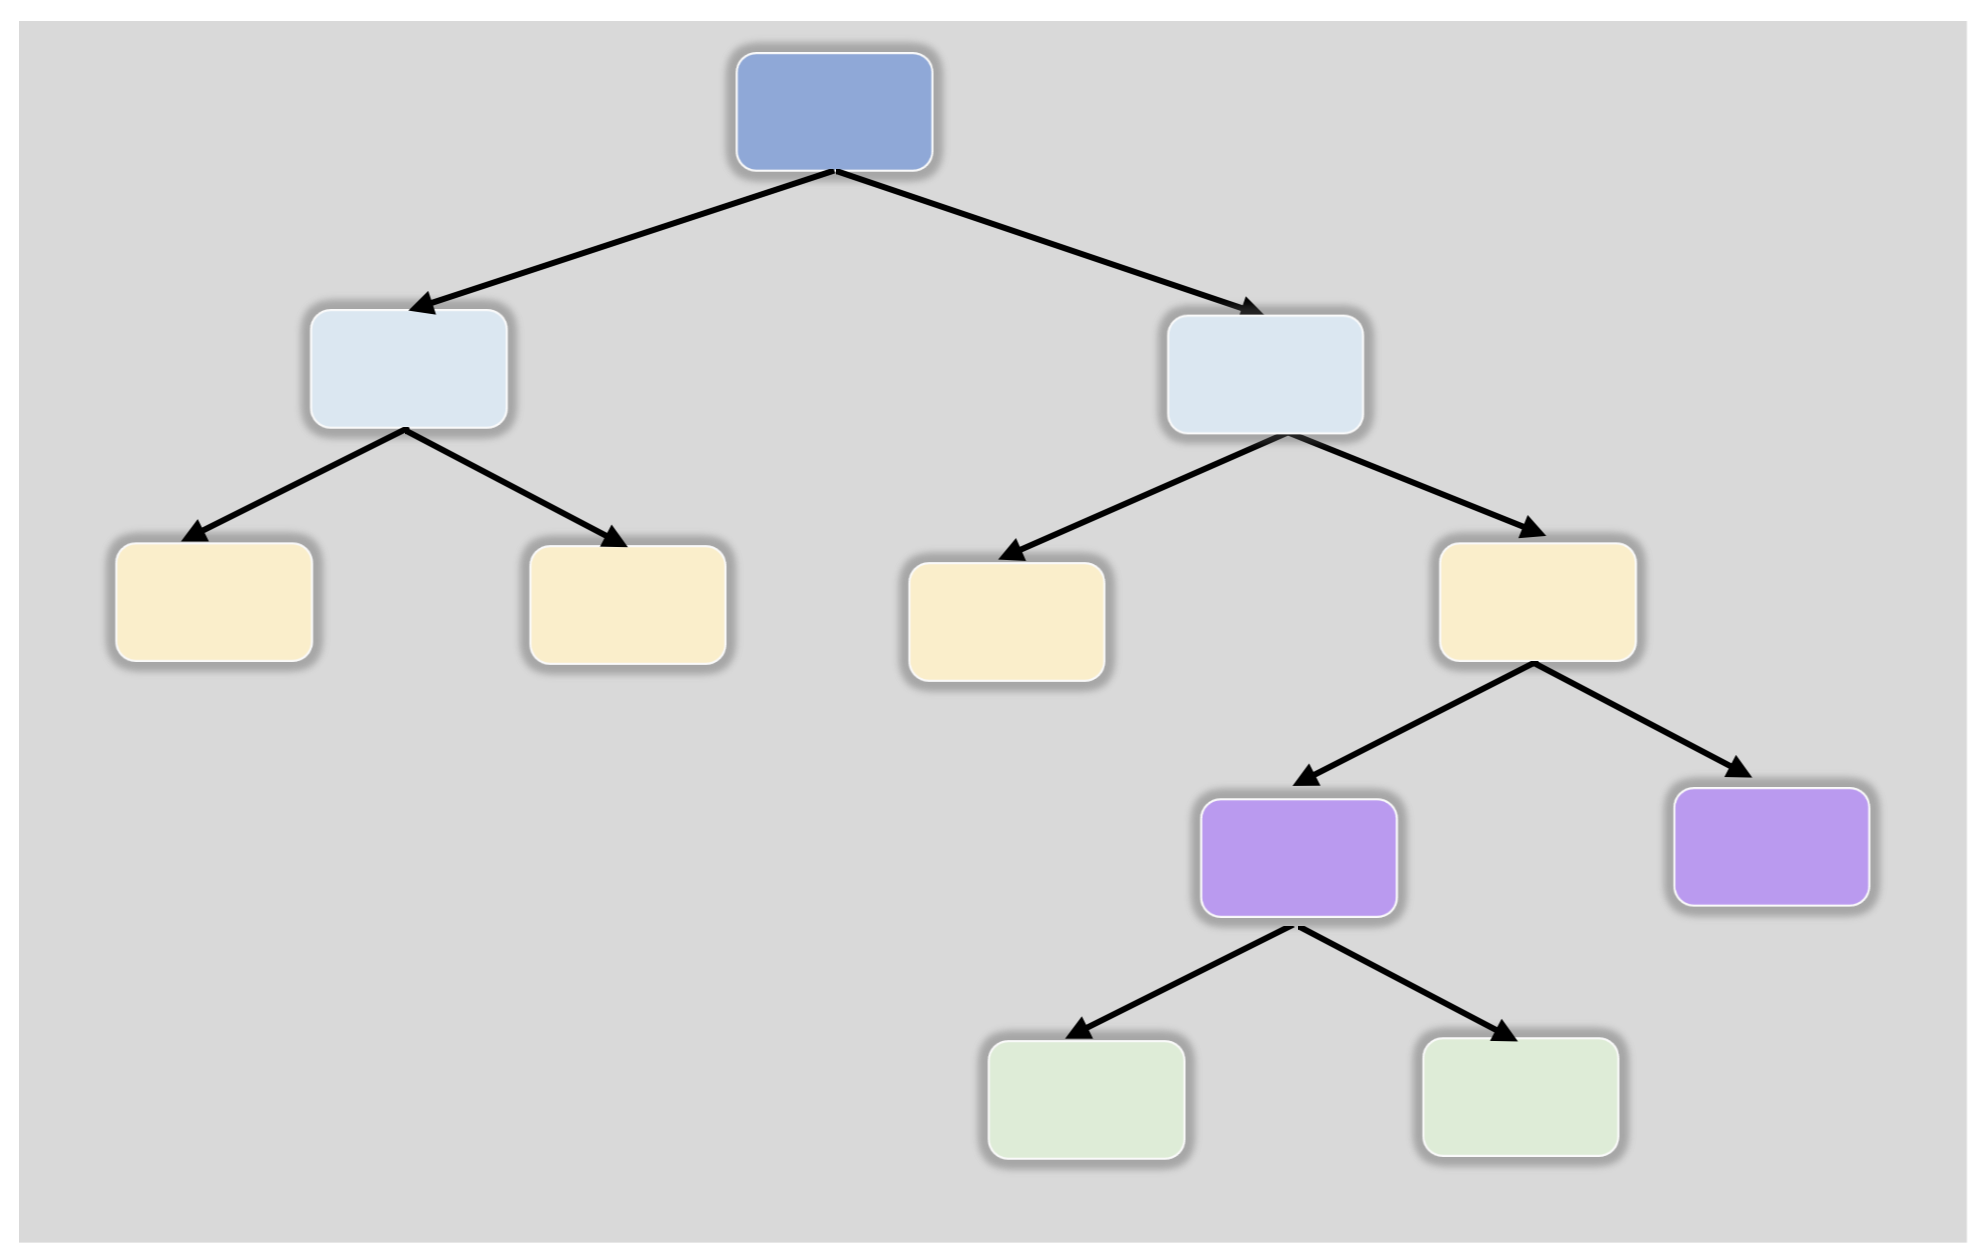
\includegraphics[scale=.15]{figs/T0.png},
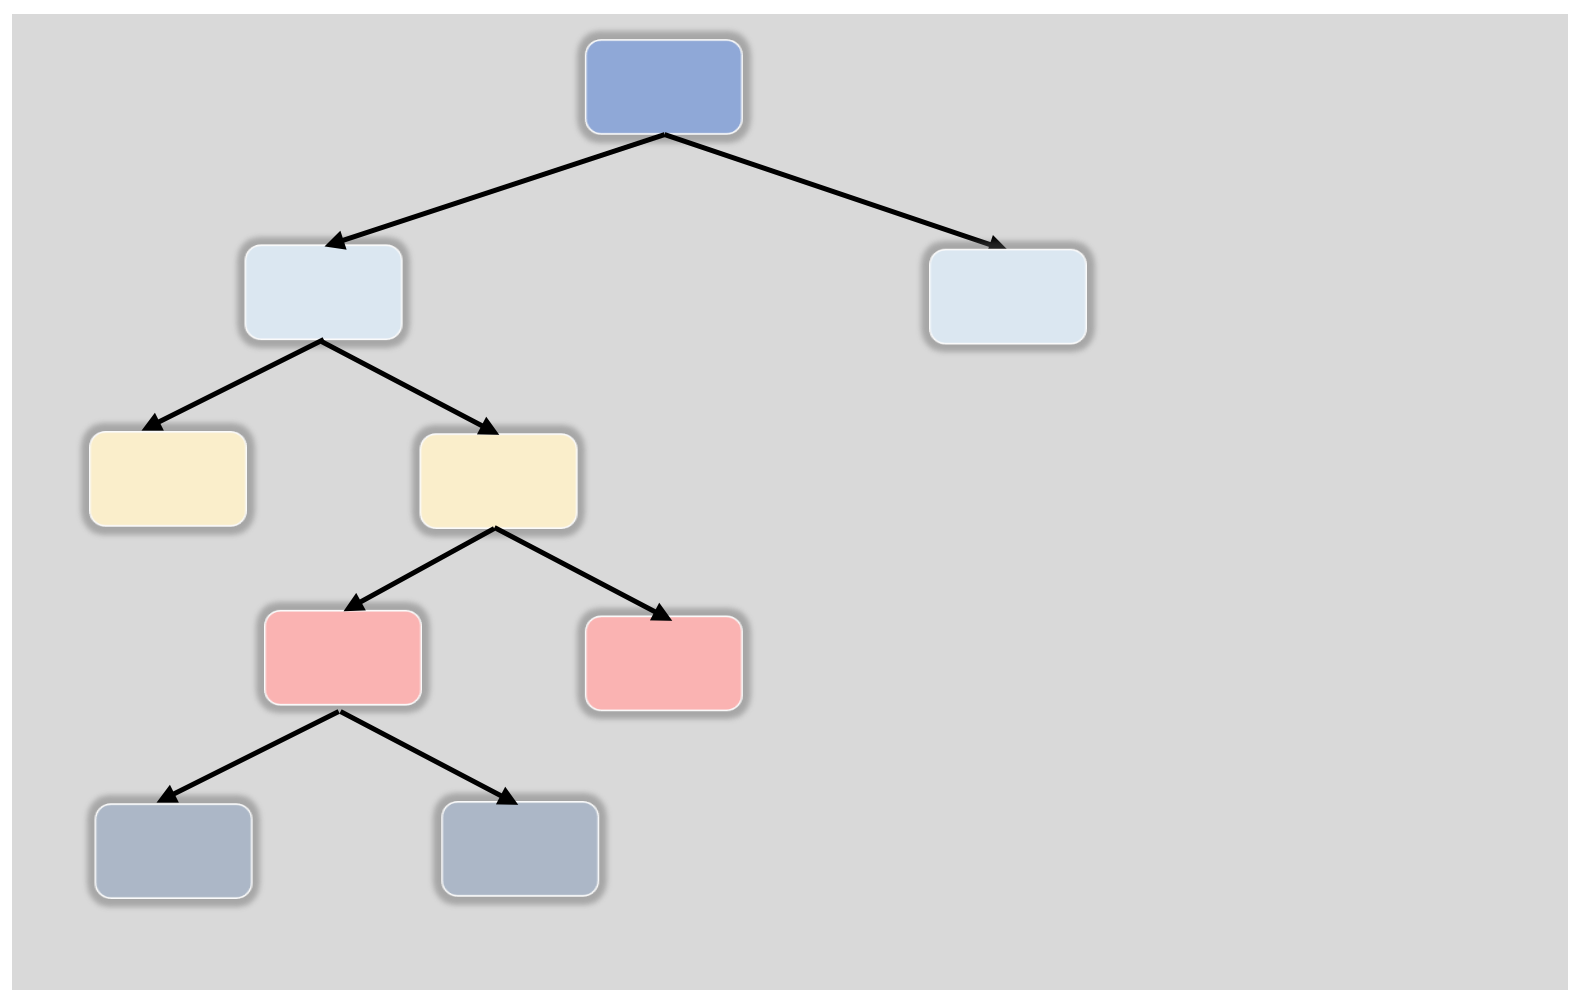
\includegraphics[scale=.28]{figs/T3.png}}$
\end{center}
}\\
\end{frame}



\begin{frame}
\qBrd[4.7in]{babyblueeyes!50}{
\begin{center}
$\Col{
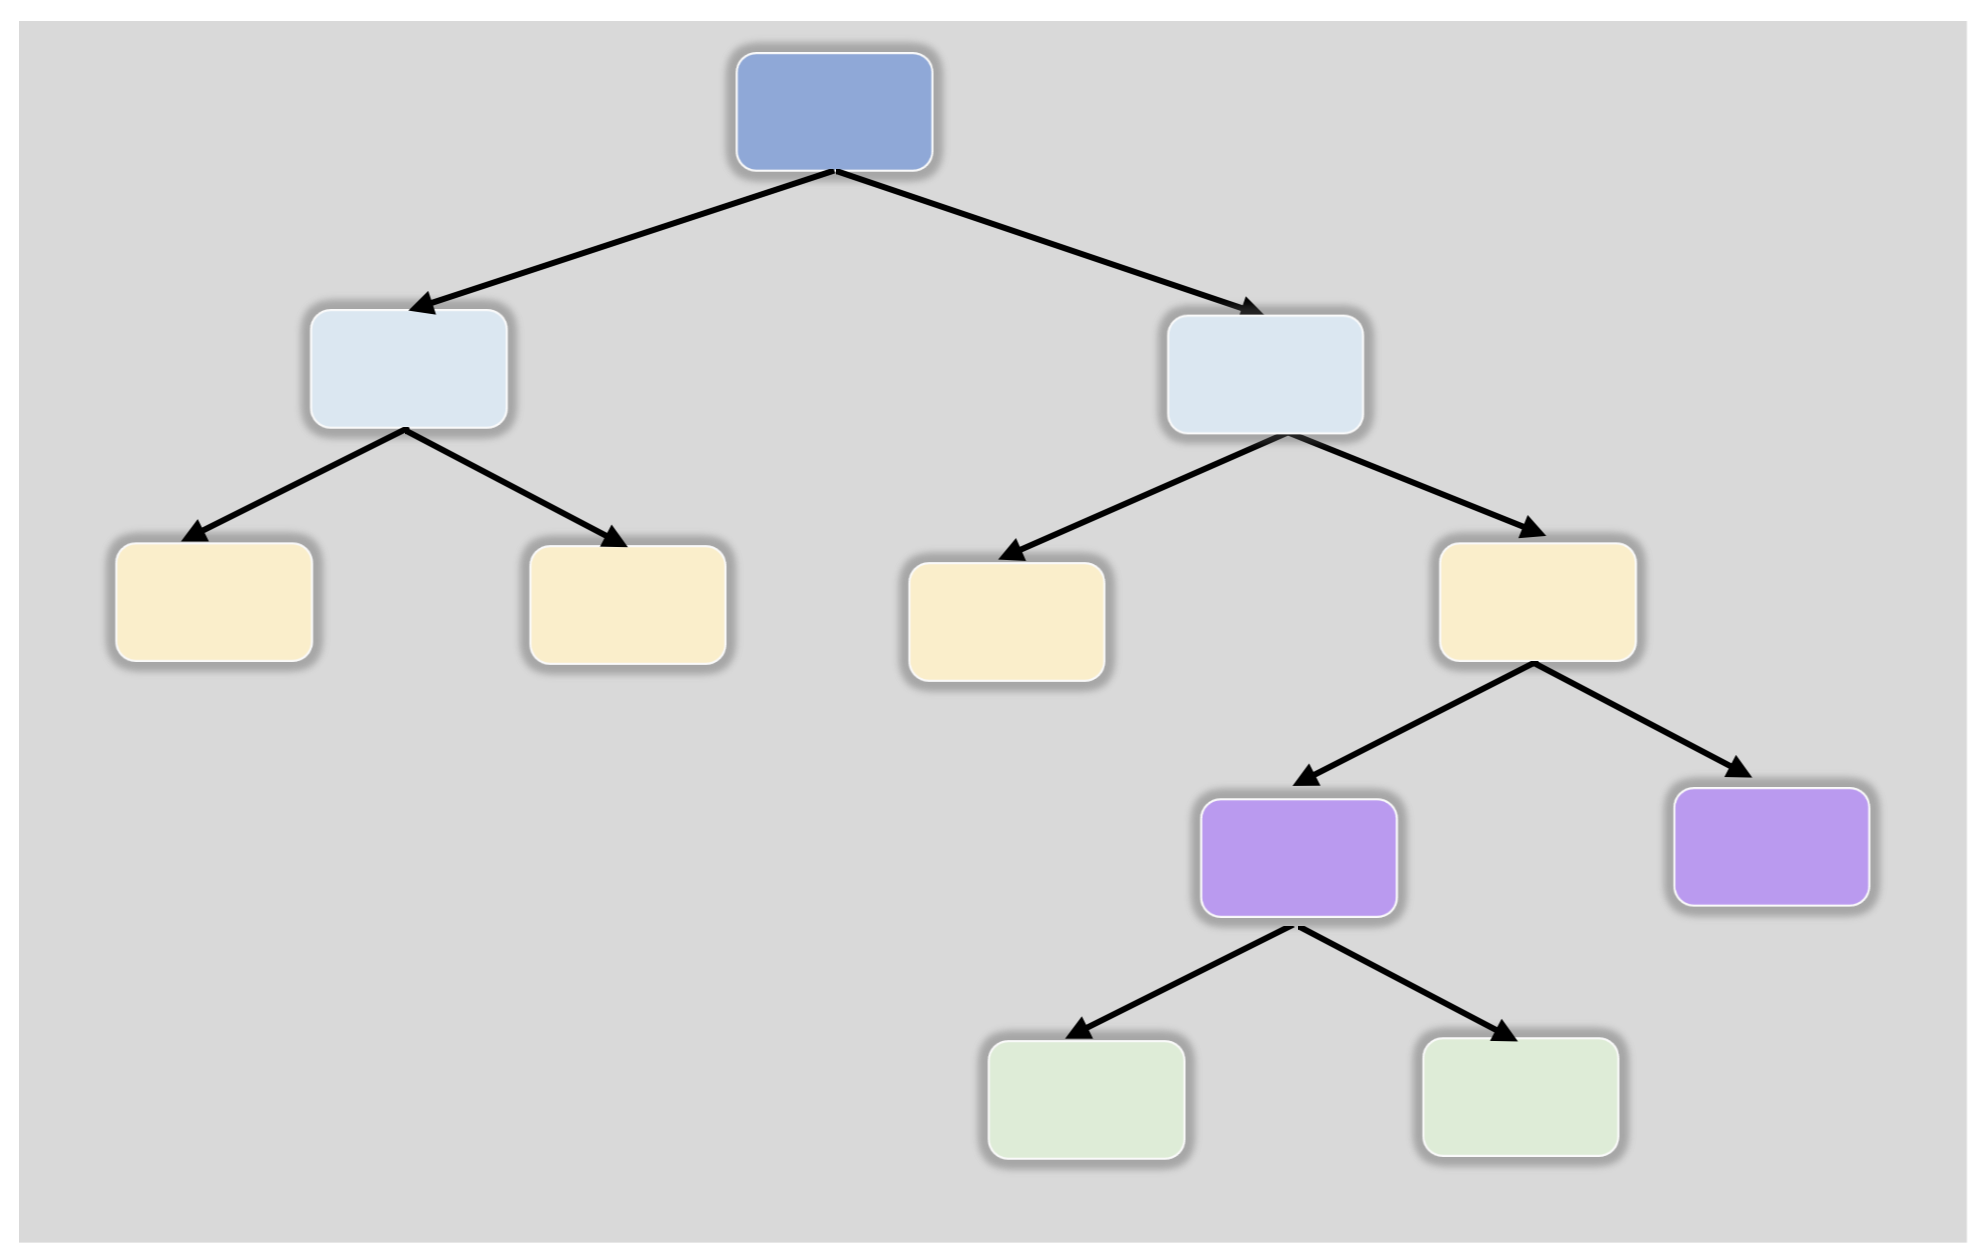
\includegraphics[scale=.15]{figs/T0.png},
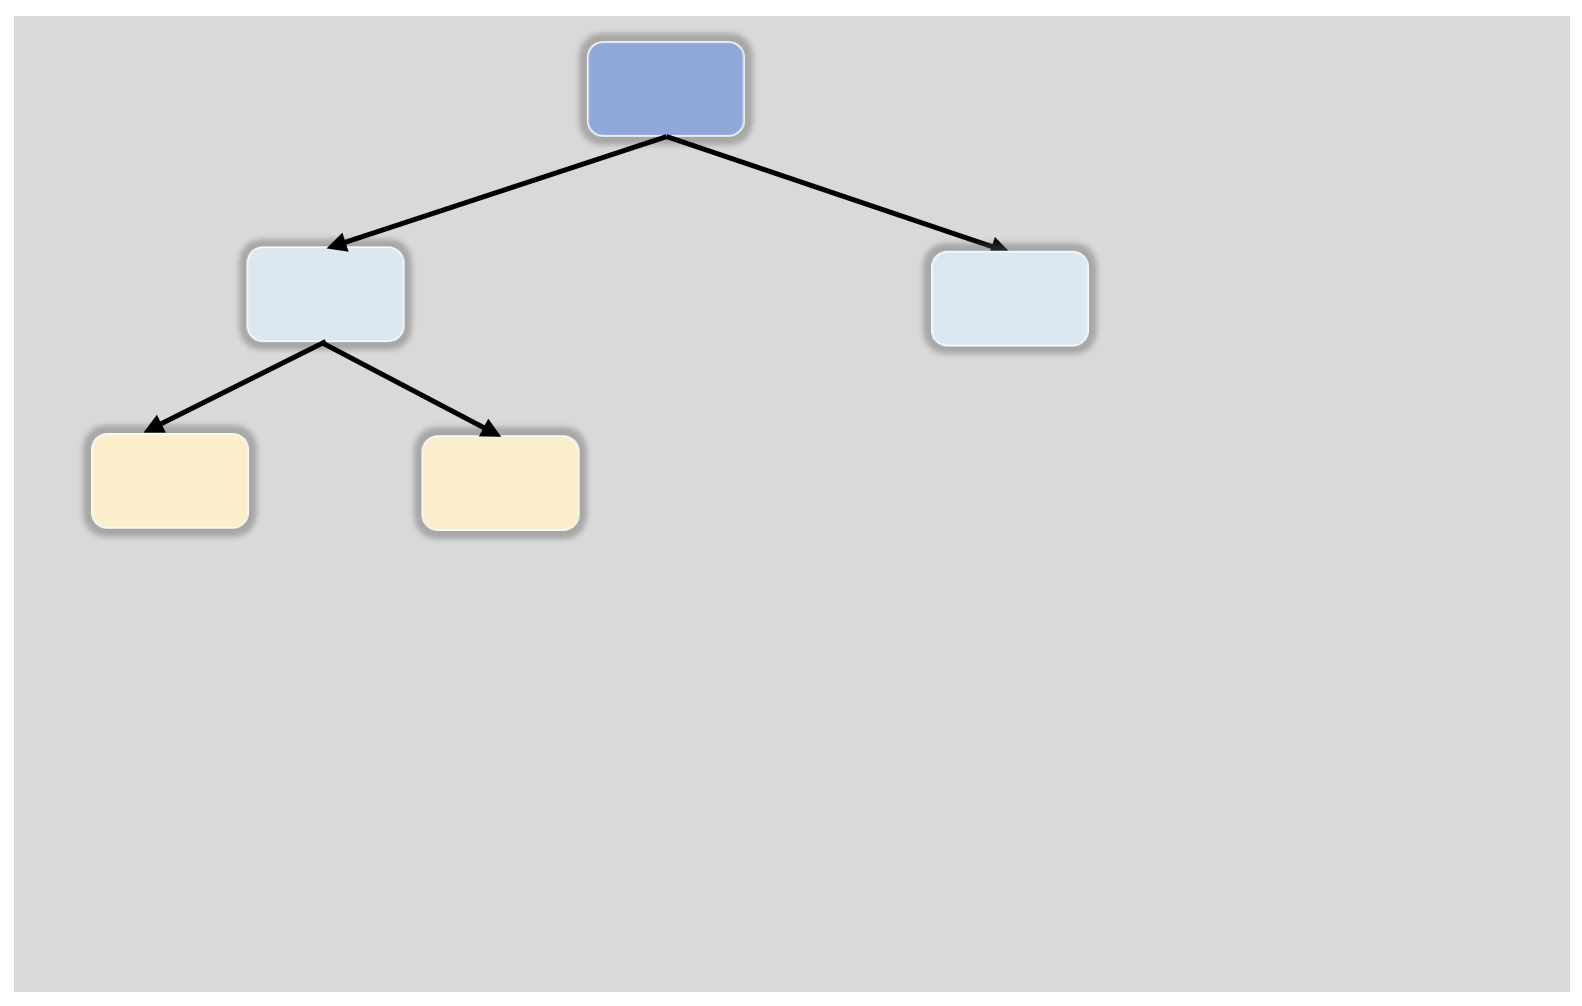
\includegraphics[scale=.28]{figs/T2.png}}$
\end{center}
}\\
\end{frame}

\TransitionFrame[olive]{\Large $\vert T \vert $: Order of a Tree  }


\begin{frame}
\qBrd[4.7in]{babyblueeyes!50}{
\begin{center}
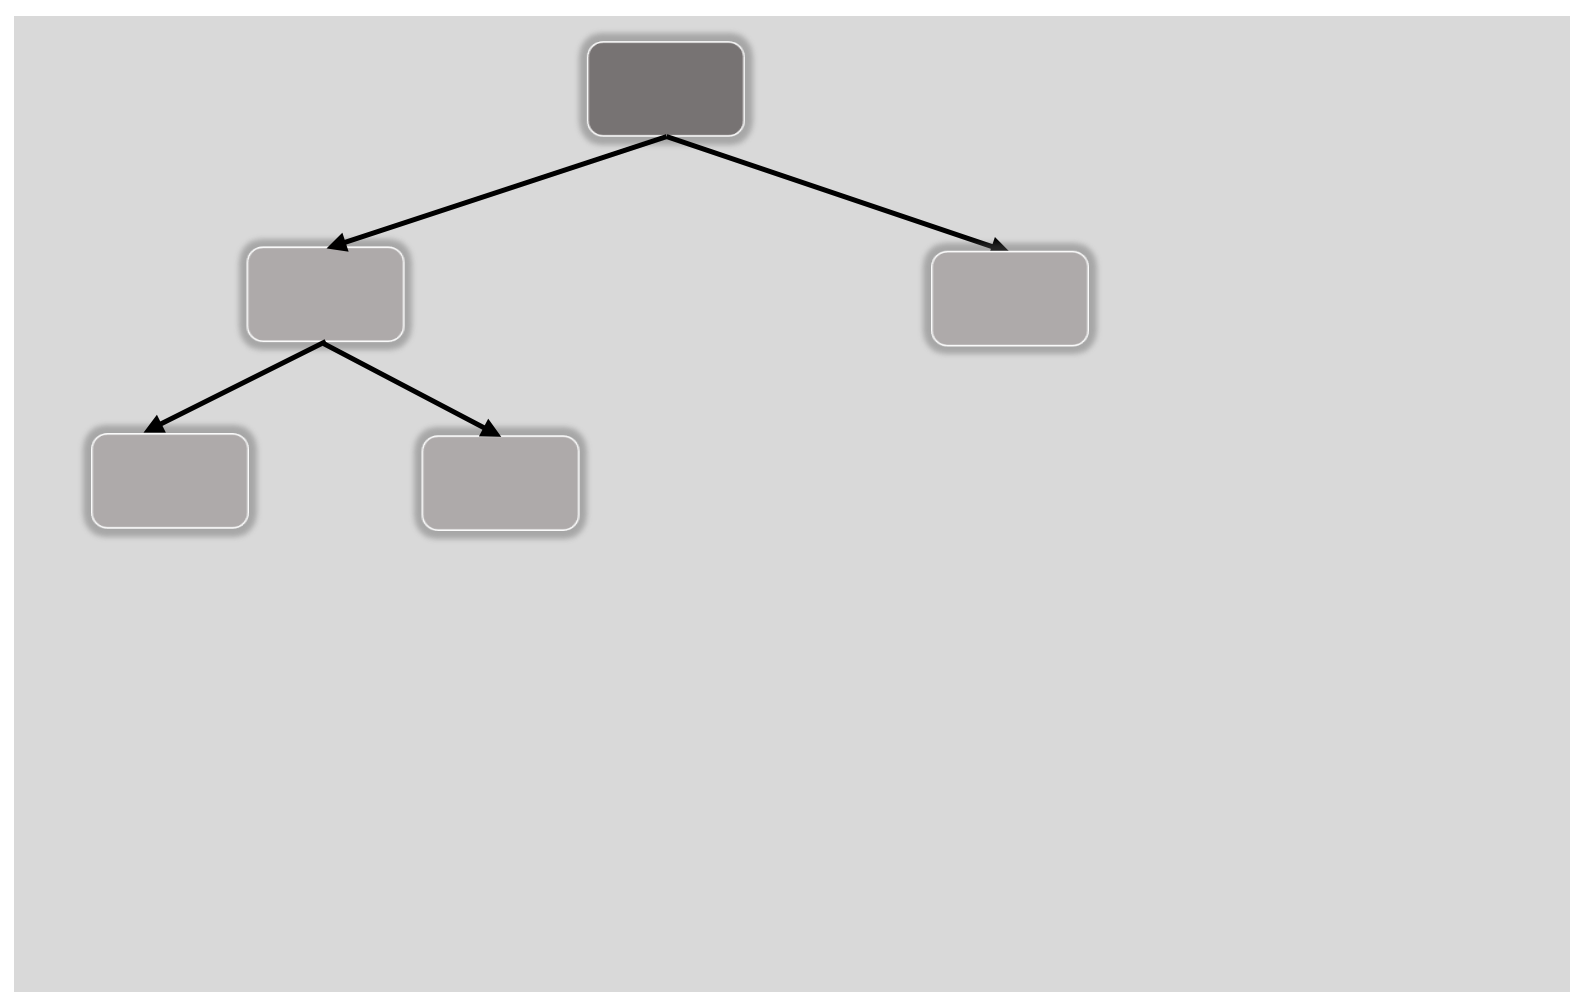
\includegraphics[scale=.4]{figs/T11_Q.png}
\end{center}
}\\
\end{frame}


\begin{frame}
\qBrd[4.7in]{babyblueeyes!50}{
\begin{center}
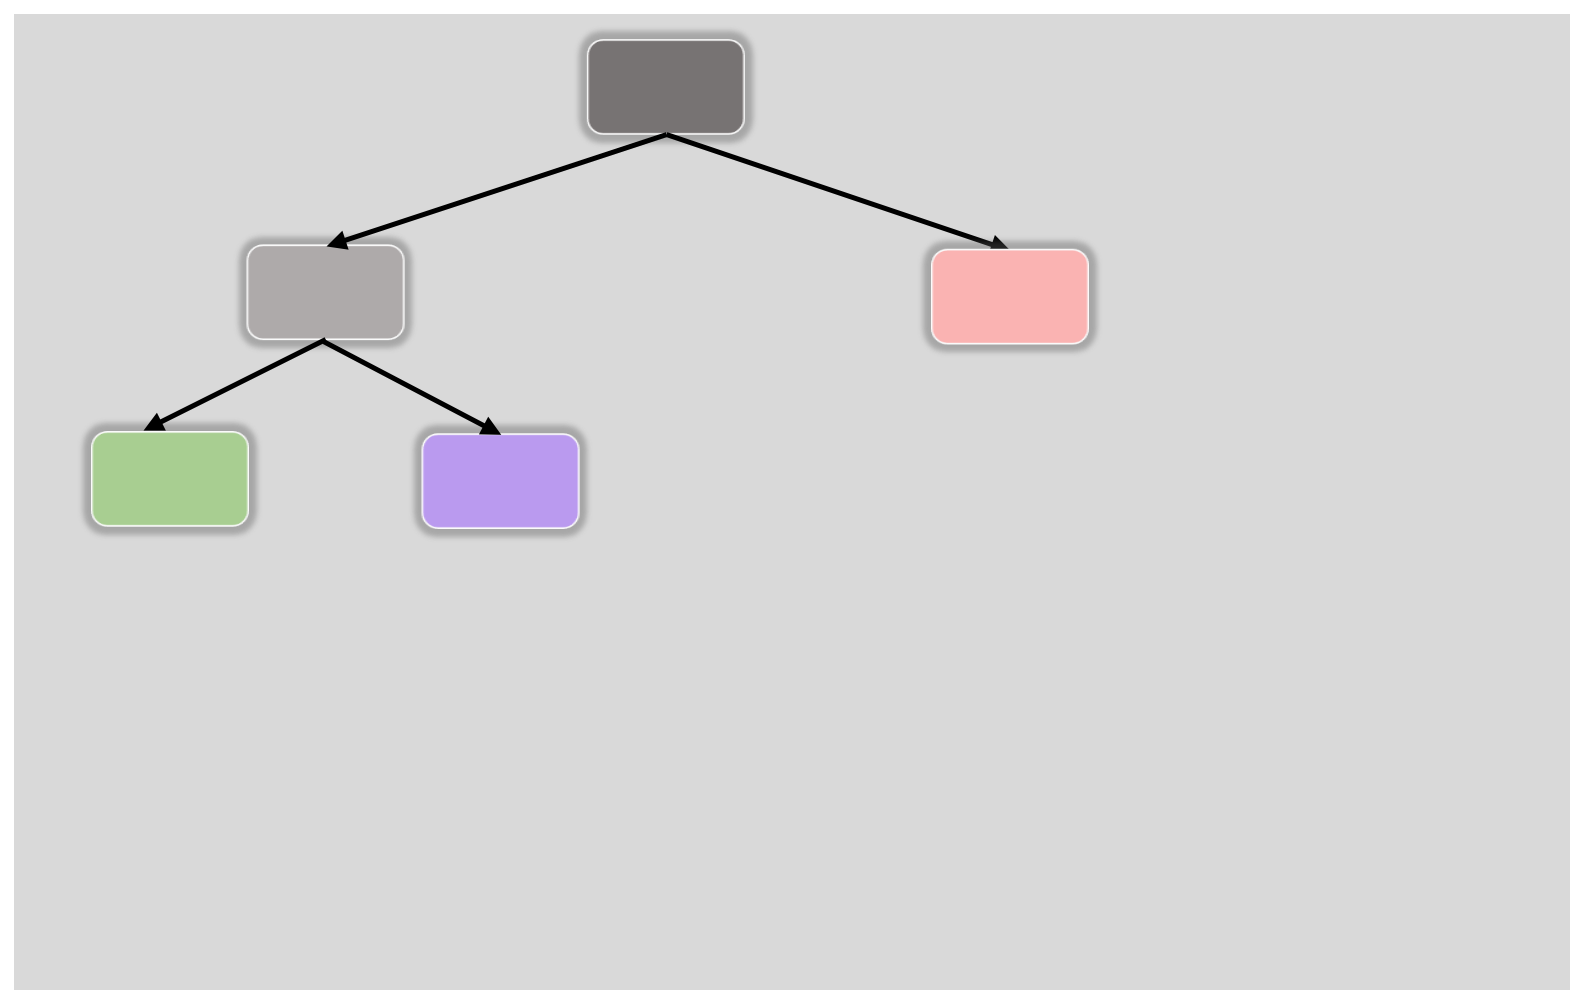
\includegraphics[scale=.4]{figs/T11_A.png}
\end{center}
}\\
\end{frame}






\begin{frame}
\qBrd[4.7in]{babyblueeyes!50}{
\begin{center}
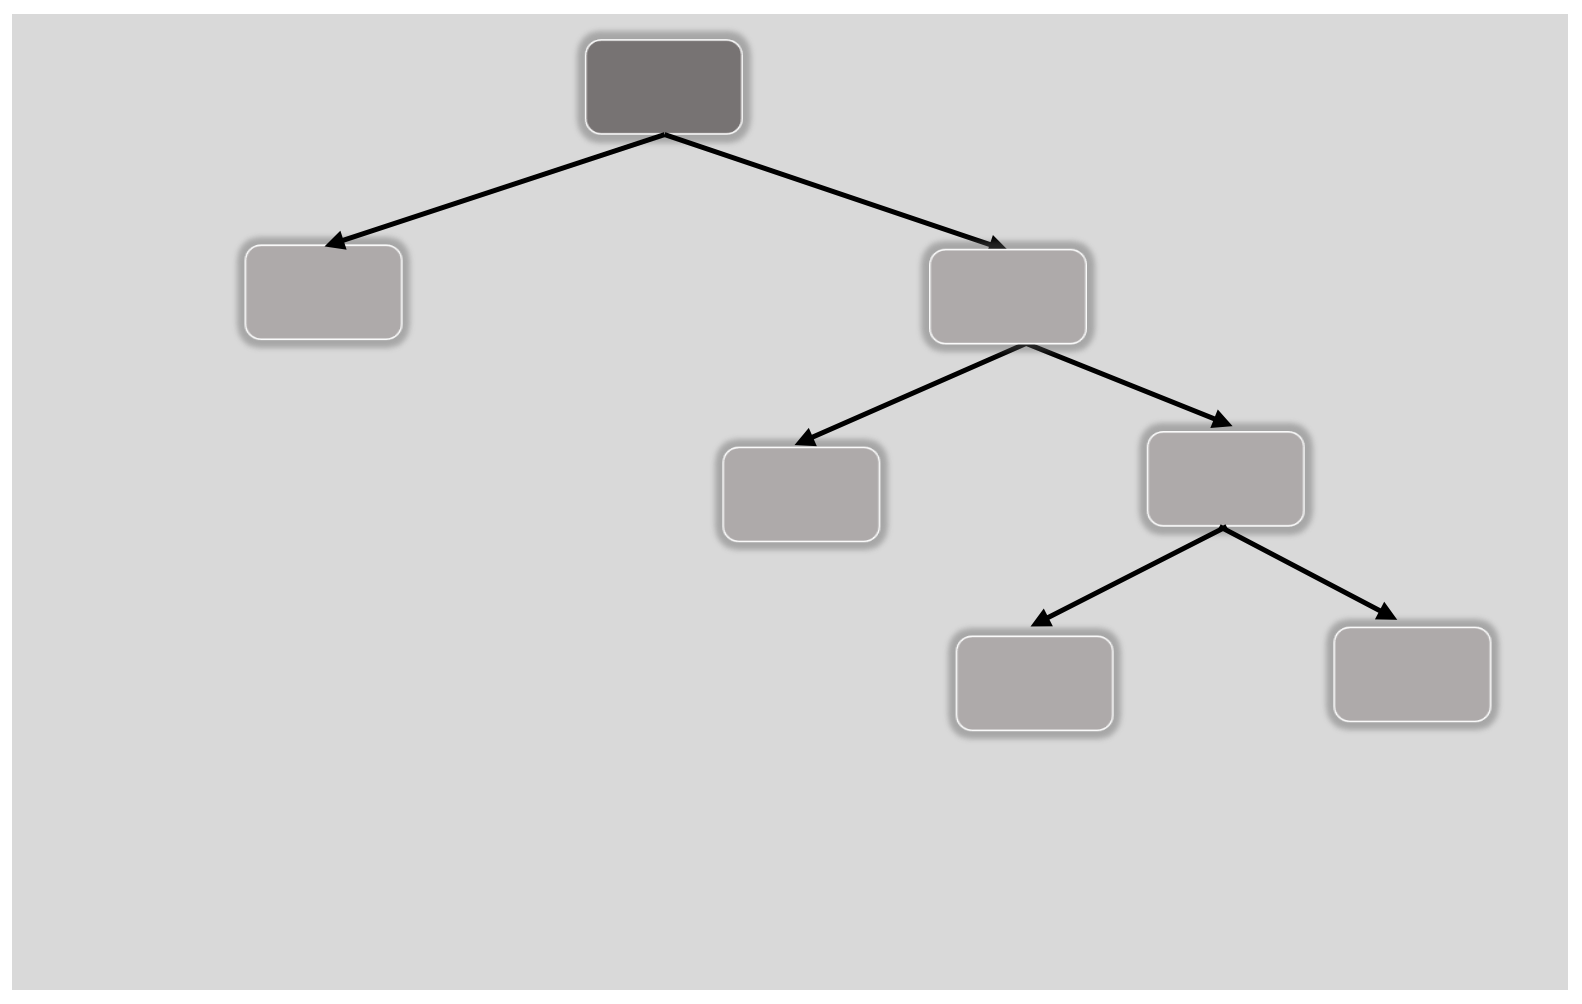
\includegraphics[scale=.4]{figs/T12_Q.png}
\end{center}
}\\
\end{frame}


\begin{frame}
\qBrd[4.7in]{babyblueeyes!50}{
\begin{center}
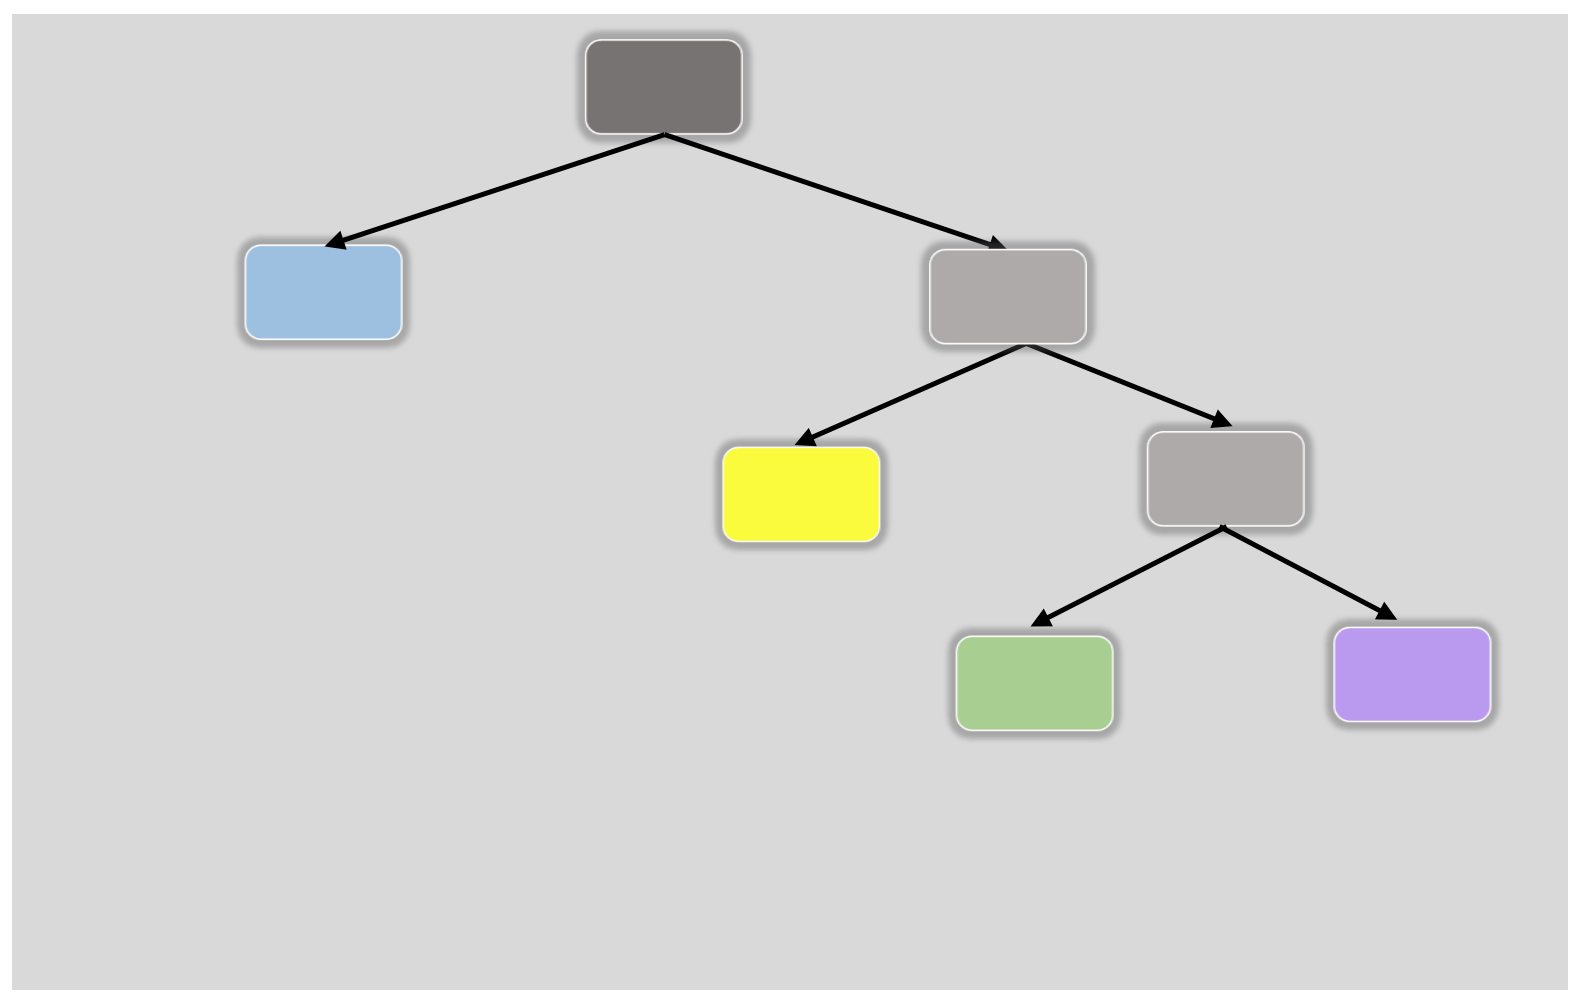
\includegraphics[scale=.4]{figs/T12_A.png}
\end{center}
}\\
\end{frame}





\begin{frame}
\qBrd[4.7in]{babyblueeyes!50}{
\begin{center}
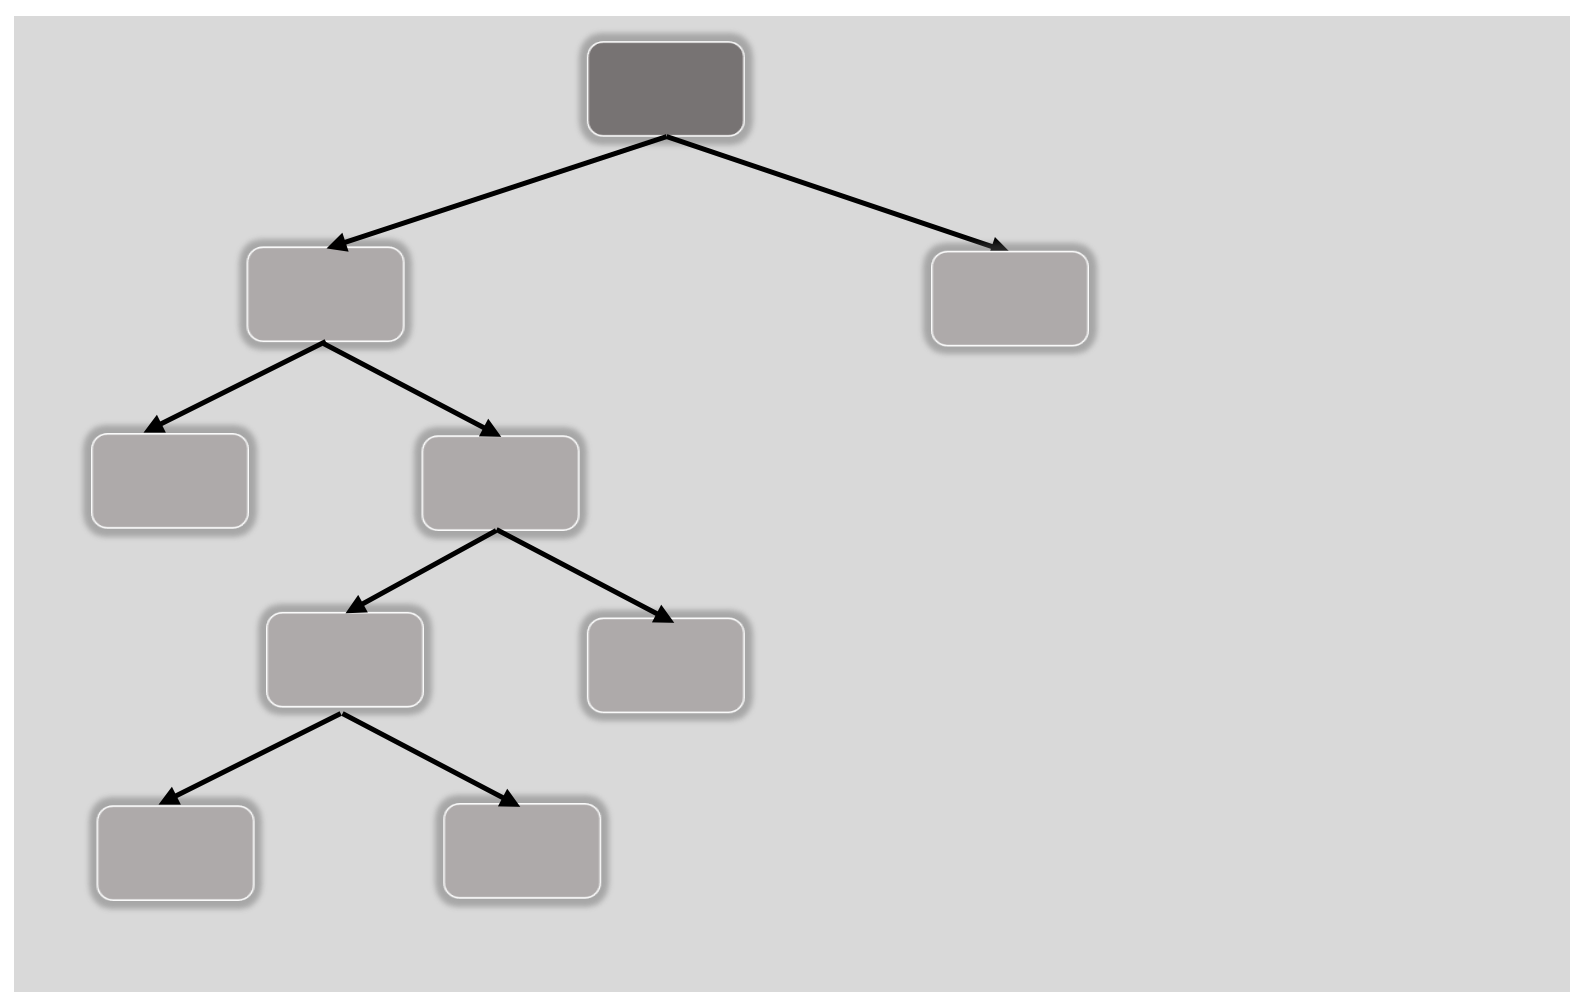
\includegraphics[scale=.4]{figs/T13_Q.png}
\end{center}
}\\
\end{frame}


\begin{frame}
\qBrd[4.7in]{babyblueeyes!50}{
\begin{center}
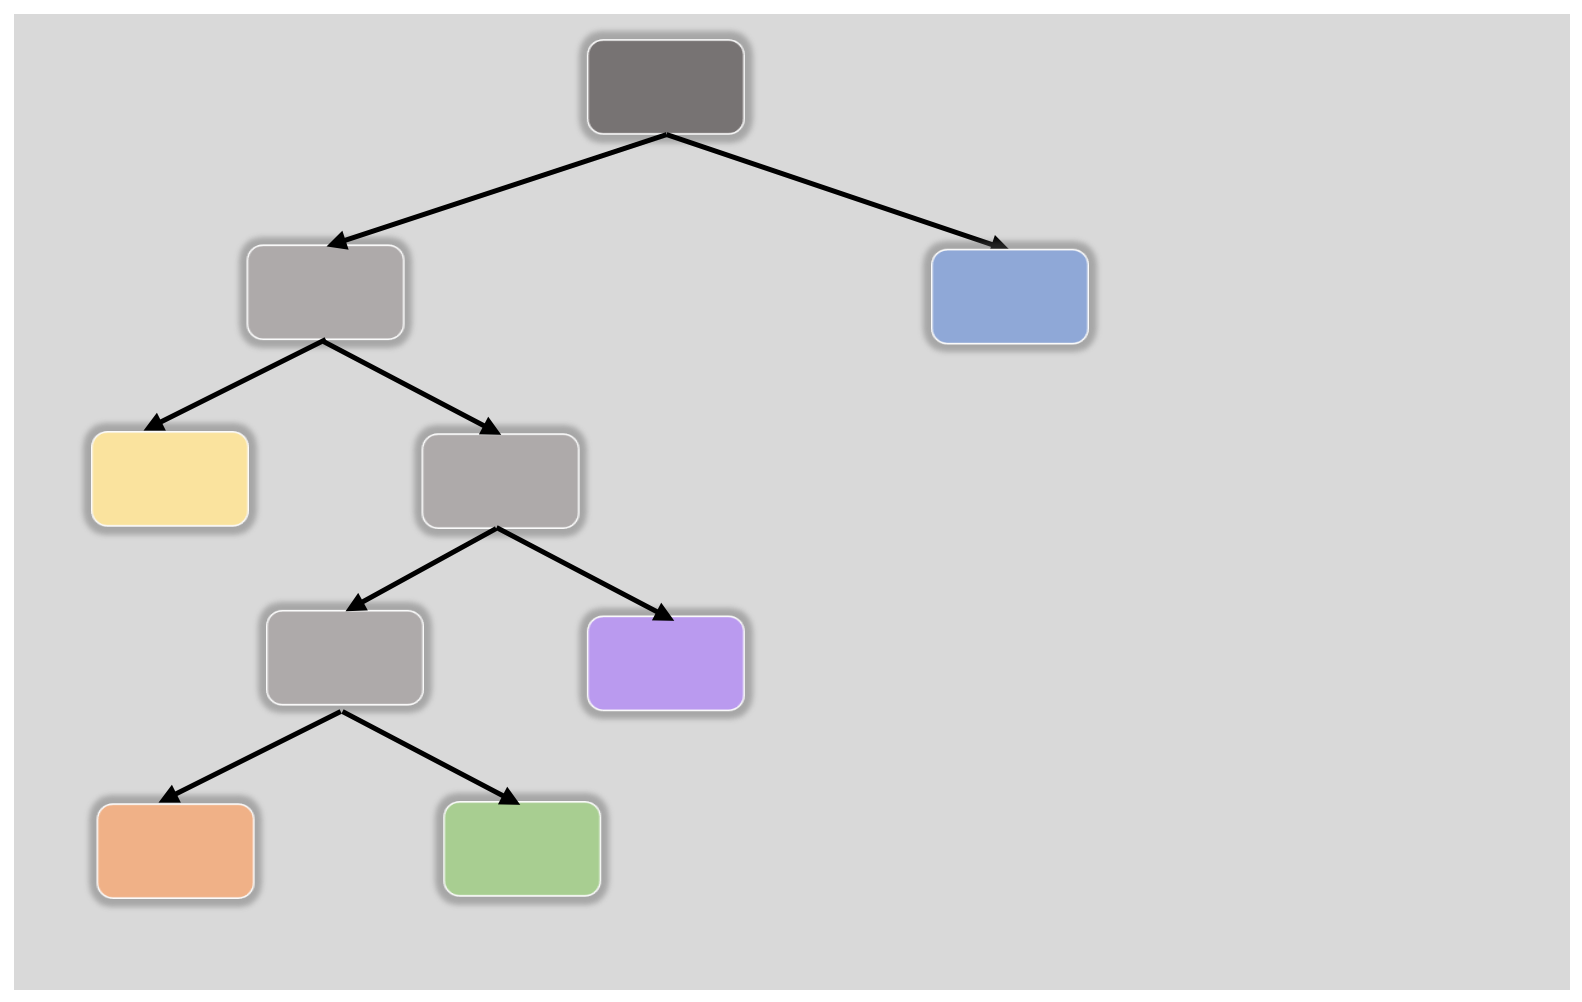
\includegraphics[scale=.4]{figs/T13_A.png}
\end{center}
}\\
\end{frame}



\begin{frame}
\qBrd[4.7in]{babyblueeyes!50}{
\begin{center}
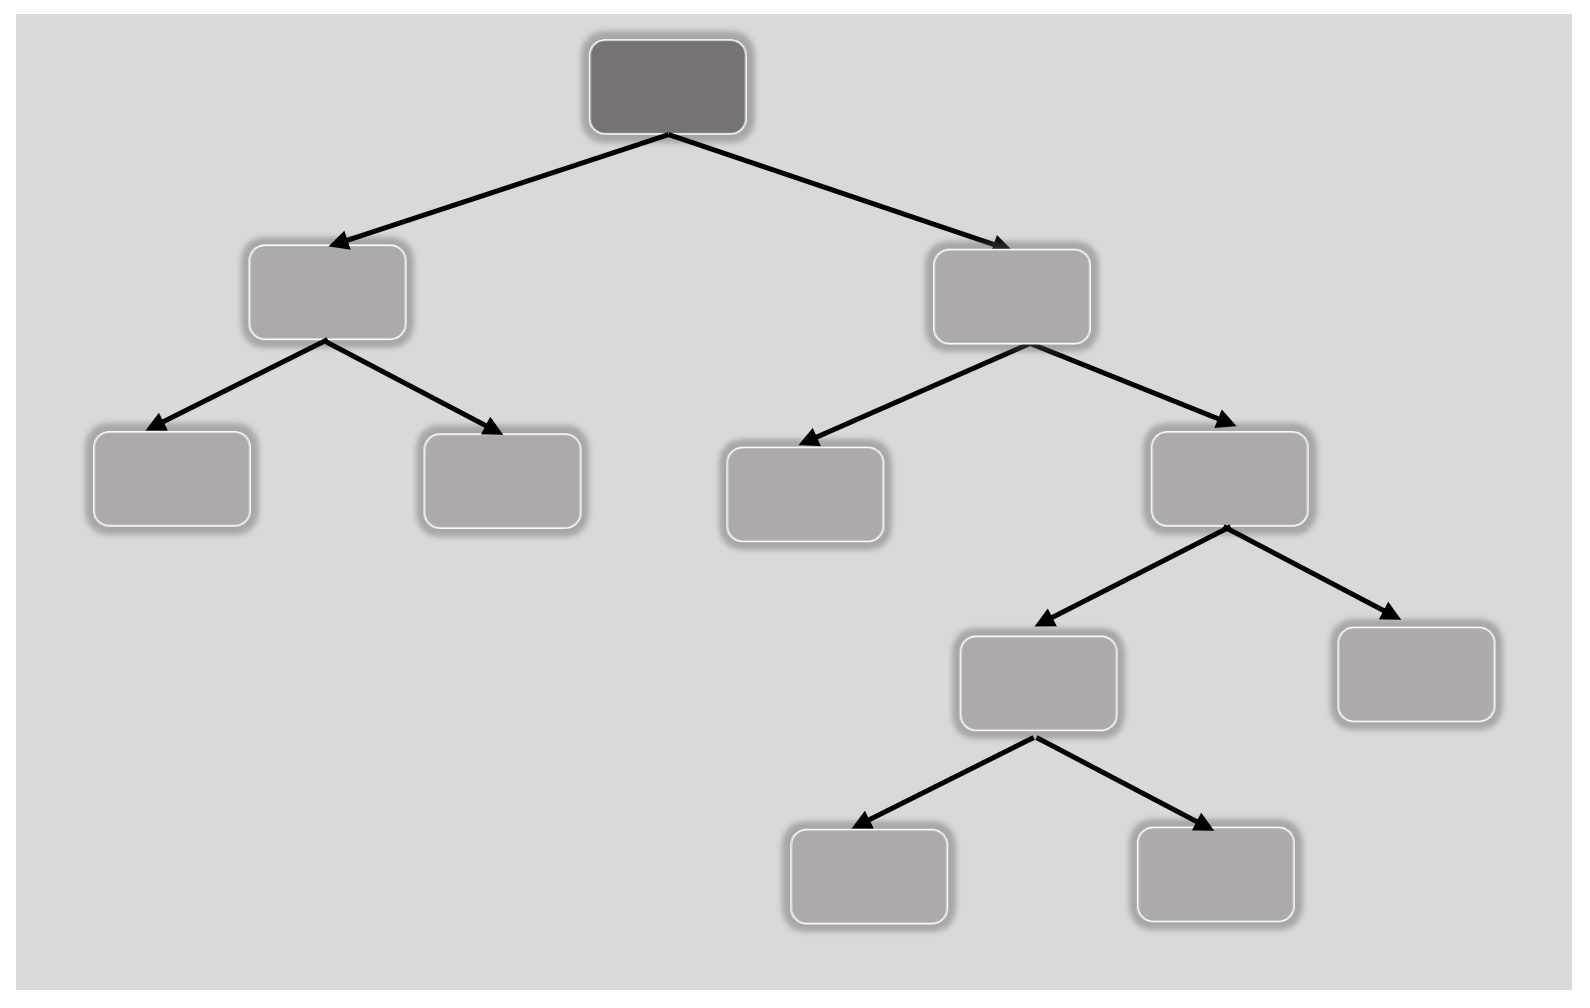
\includegraphics[scale=.4]{figs/T14_Q.png}
\end{center}
}\\
\end{frame}


\begin{frame}
\qBrd[4.7in]{babyblueeyes!50}{
\begin{center}
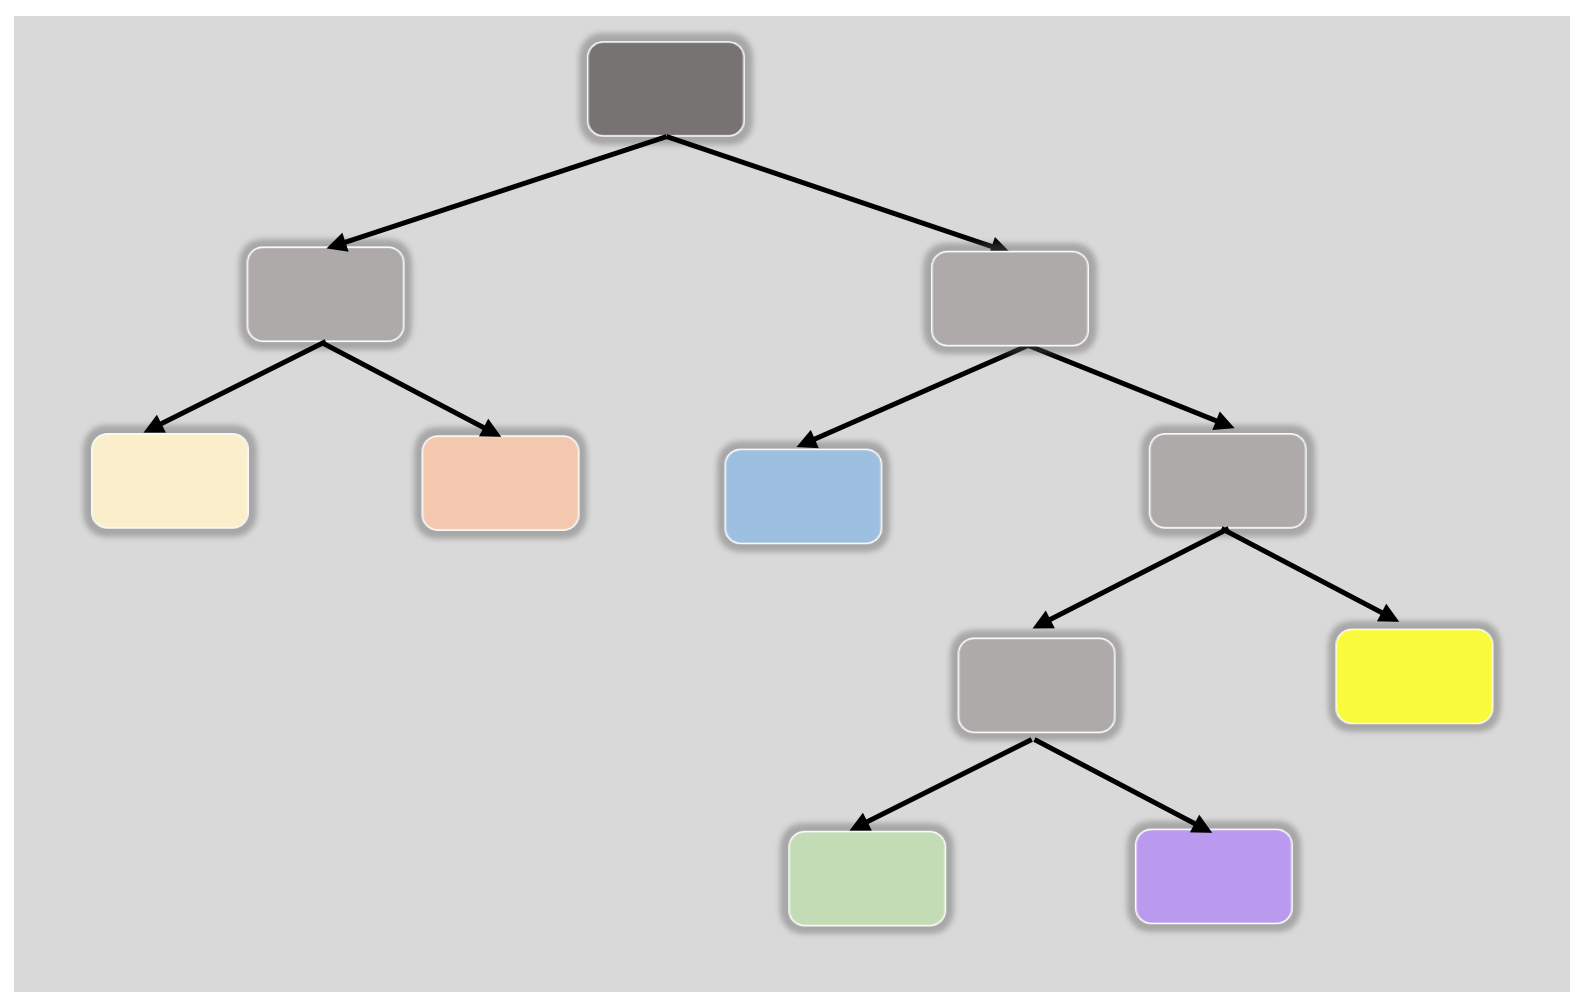
\includegraphics[scale=.4]{figs/T14_A.png}
\end{center}
}\\
\end{frame}




\TransitionFrame[antiquebrass]{\Large  Tree Pruning }
%


{ \setbeamercolor{background canvas}{bg=}
\includepdf[pages={84-84}, scale=1]{STAT380-Unit3.pdf}
}



\begin{frame}
\qBrd[4.1in]{babyblueeyes!60}{ $$\HLTW{ \displaystyle
\mathcal{C}ost(T):}=   \DBX{\HLTW{ \displaystyle \sum_{j=1}^{\vert T \vert } \sum_{i\in \HLTEQ[rose!40]{\HLTY{ R_j}}}^{}\left(y_i - \HLTY{ \widehat{c}_j} \right)^2  } +\HLTW{\alpha \vert  T \vert}} \text{ where } \DBX{ \HLTY{ \displaystyle  \widehat{c}_j}  =  \frac{\sum_{i \in R_j } y_i }{n_j}    }$$}\\

 \begin{center}
 
 \qBrd[2.5in]{olive!60}{ 
 \begin{center}
 $\DBX{  \displaystyle T_{\alpha, {_\text{opt}}} = \argmin_{T \subseteq T_0 } \HLTW{\mathcal{C}ost(T)}}$
  \end{center}
 }
 \end{center}
 
 

\end{frame}


{ \setbeamercolor{background canvas}{bg=}
\includepdf[pages={85-92}, scale=1]{STAT380-Unit3.pdf}
}




\section{Classification Tree}

\TransitionFrame[antiquebrass]{\Large Classification Tree }

{ \setbeamercolor{background canvas}{bg=}
\includepdf[pages={93-94}, scale=1]{STAT380-Unit3.pdf}
}


\begin{frame}\frametitle{Classification Tree:Schematic Diagrams}
%\vspace{-.1in}
%\qBrd[4.7in]{babyblueeyes!50}{
\begin{center}
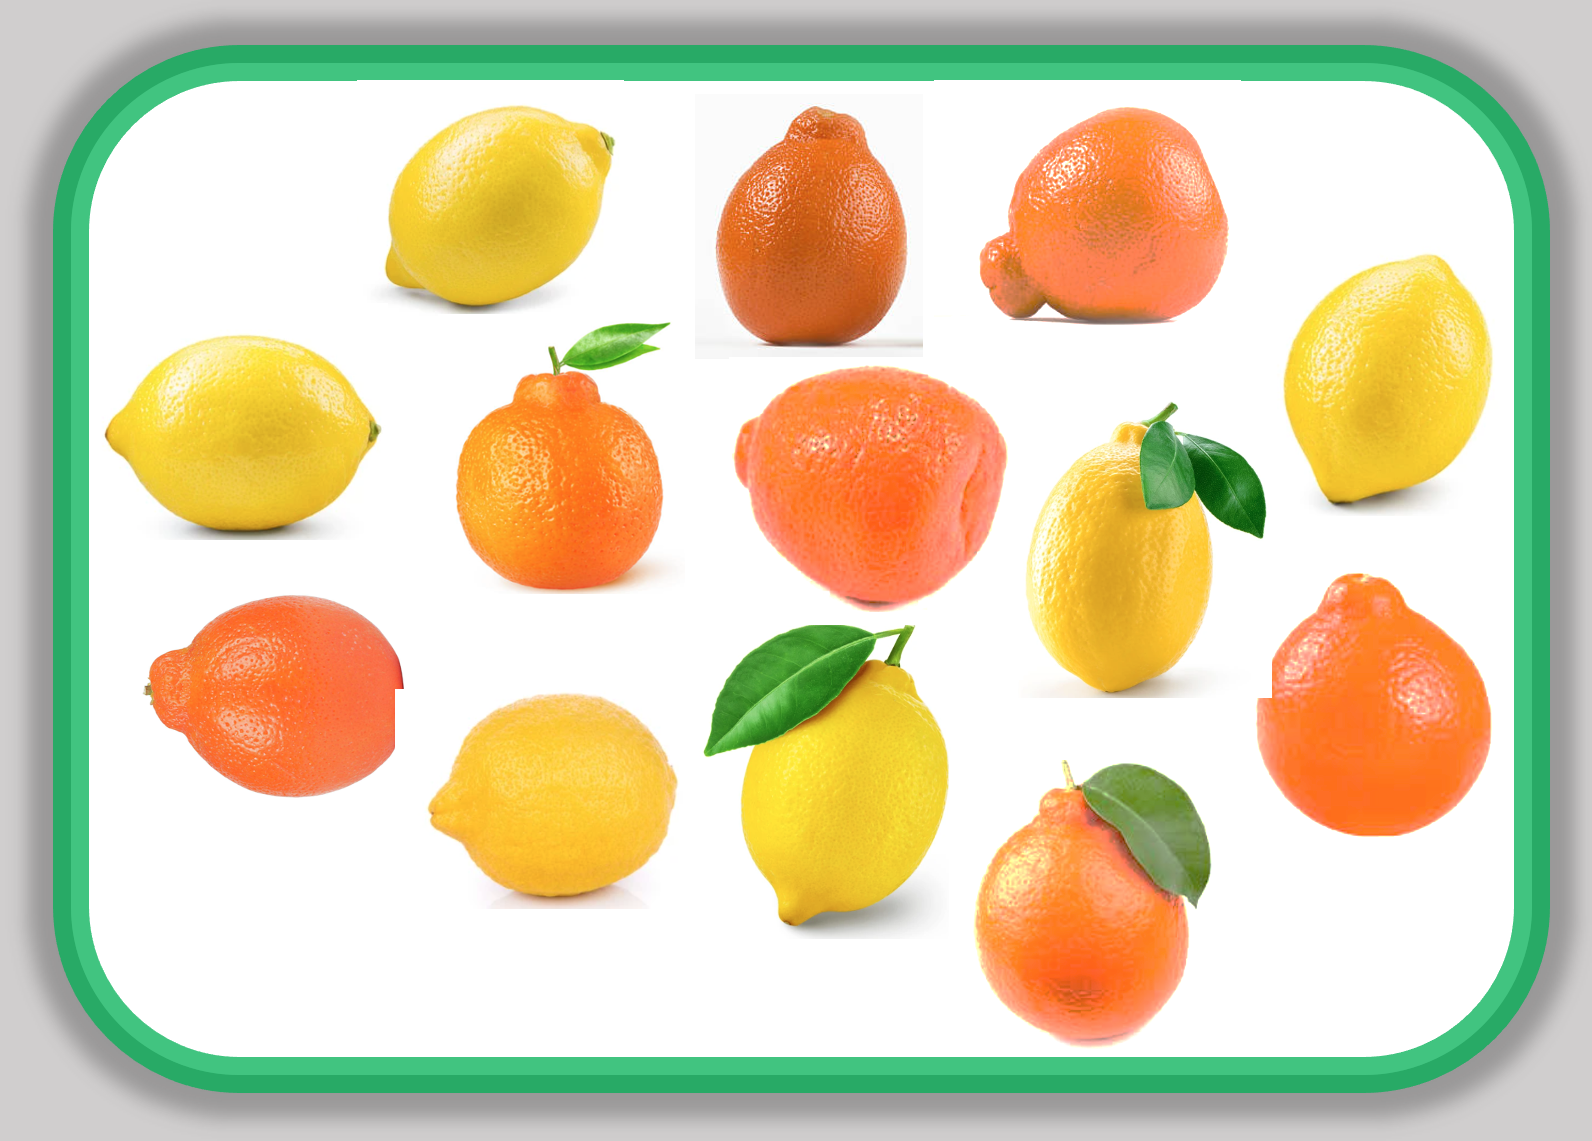
\includegraphics[scale=.3]{figs/Lemon Orange.png}
\end{center}
%}\\
\vspace{.9in}

\end{frame}












\begin{frame}\frametitle{Classification Tree:Schematic Diagrams}
%\vspace{-.1in}
%\qBrd[4.7in]{babyblueeyes!50}{
\begin{center}
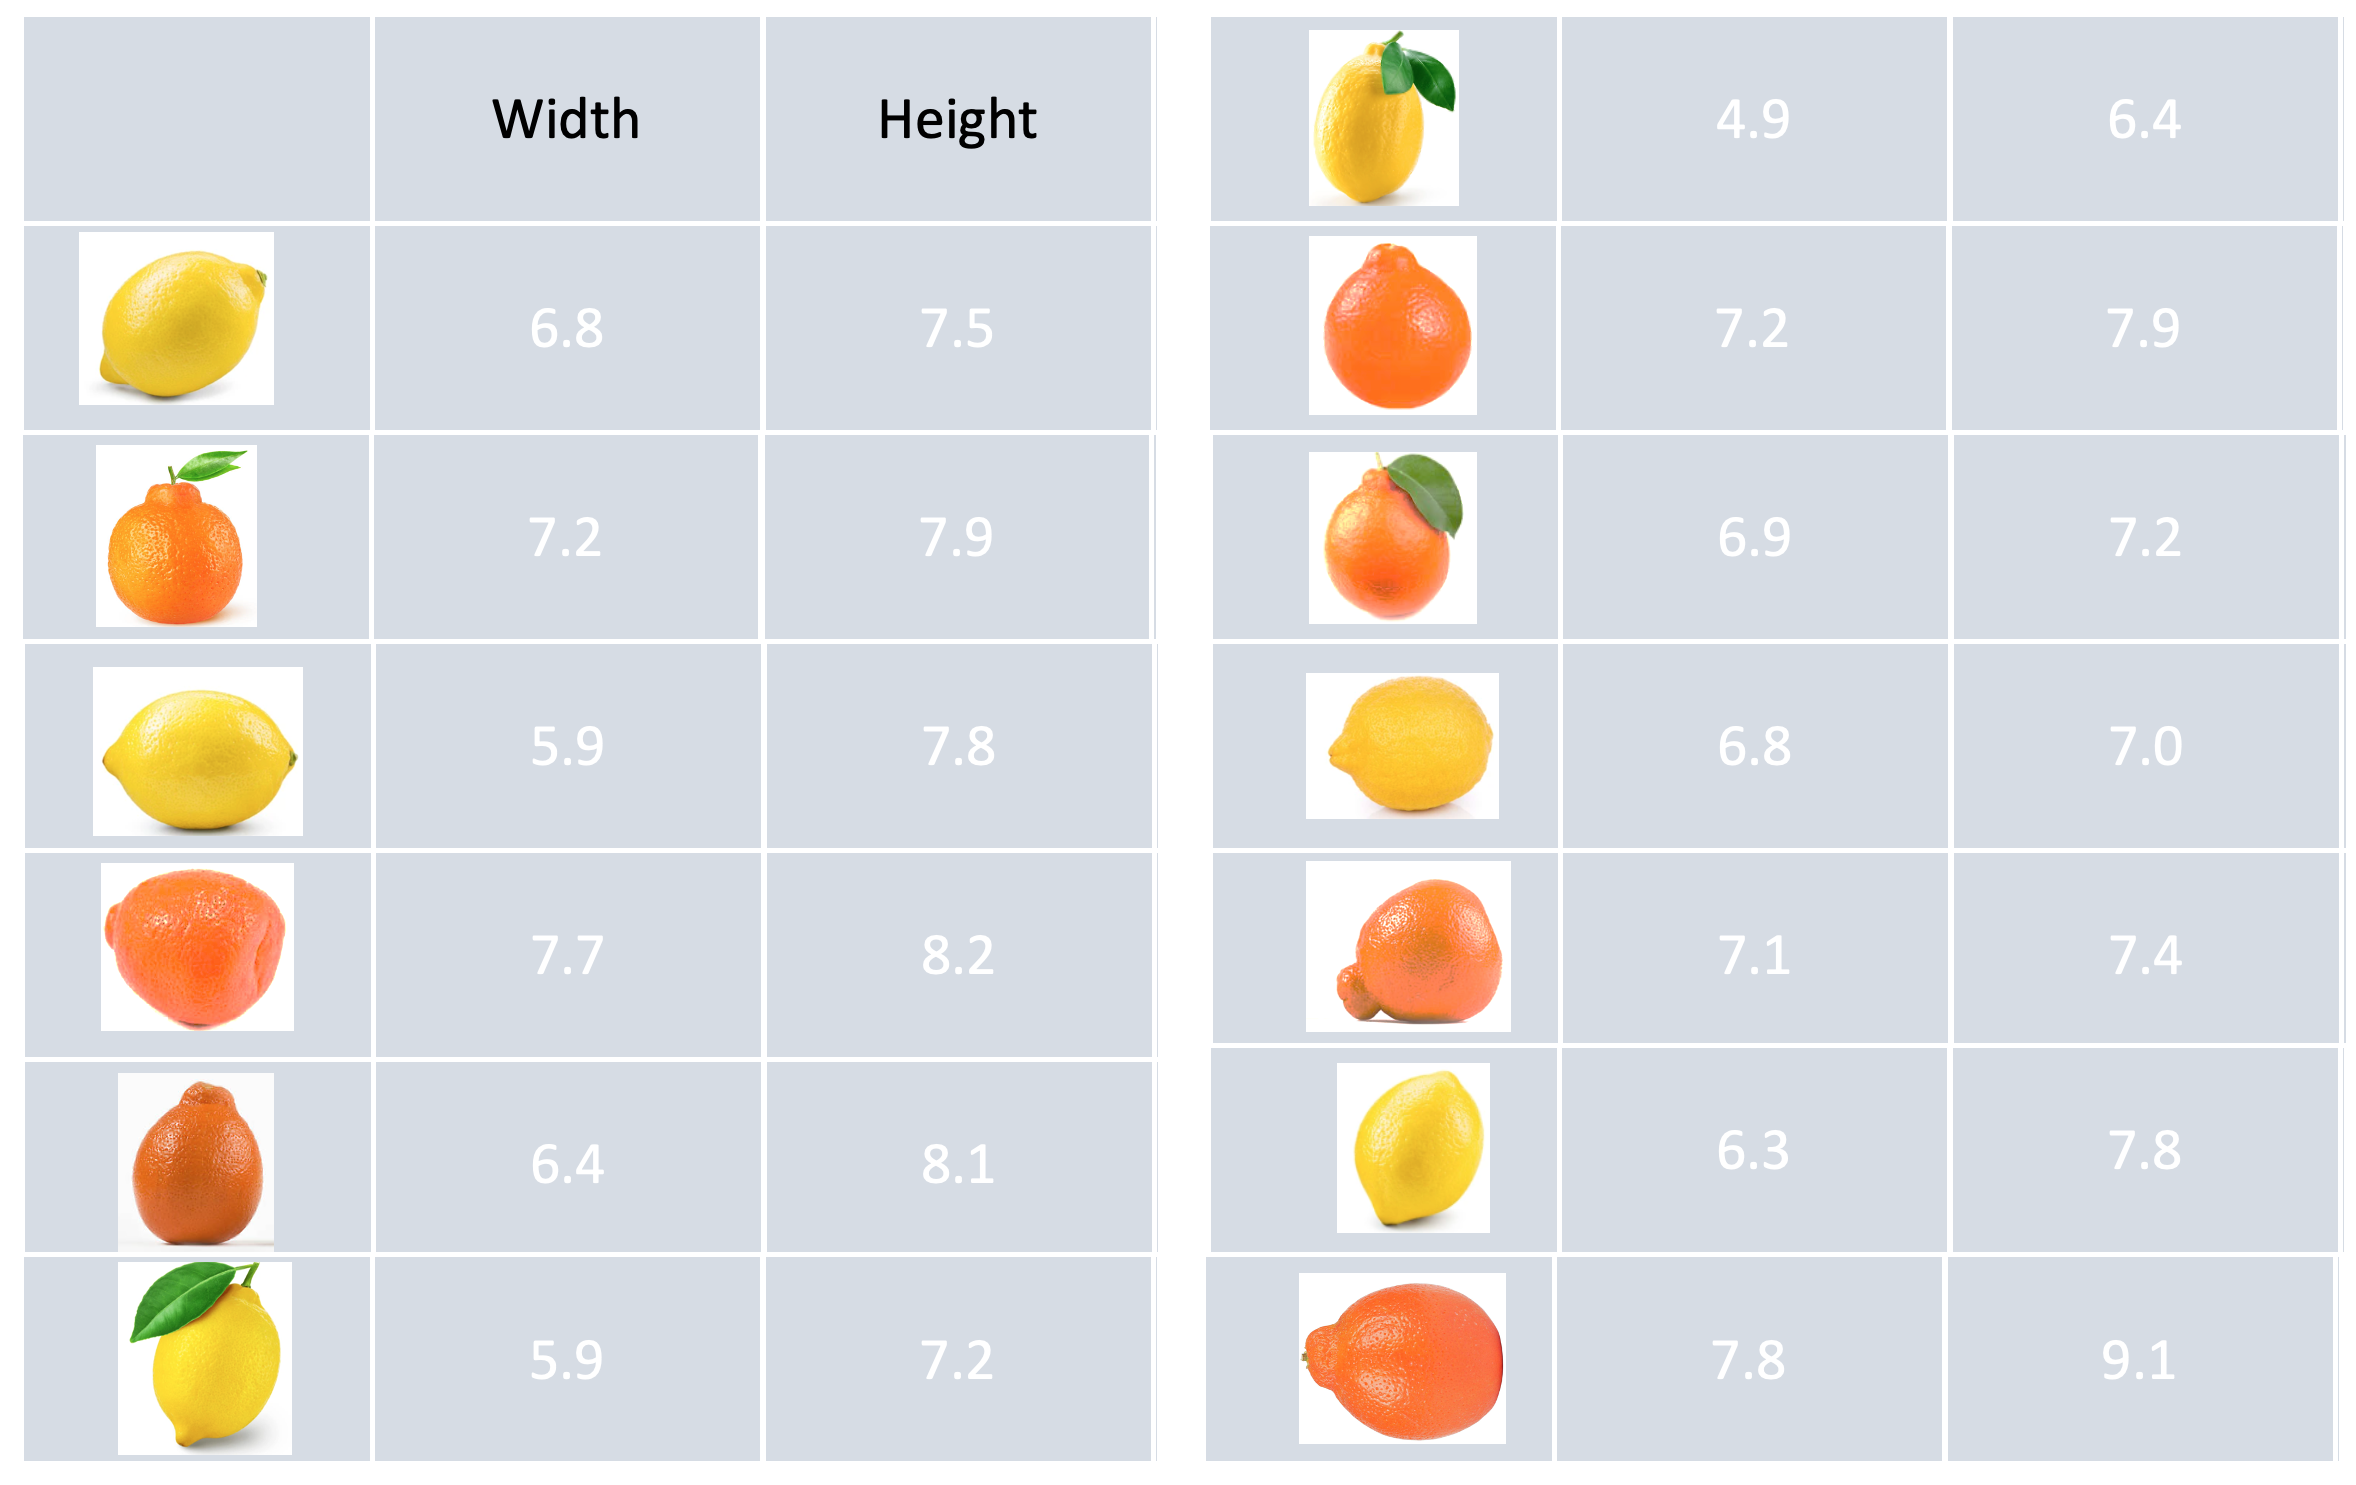
\includegraphics[scale=.25]{figs/Lemon_Orange_mock_Data.png}
\end{center}
%}\\
\vspace{.9in}

\end{frame}








\begin{frame}\frametitle{Classification Tree:Schematic Diagrams}
%\vspace{-.1in}
%\qBrd[4.7in]{babyblueeyes!50}{
\begin{center}
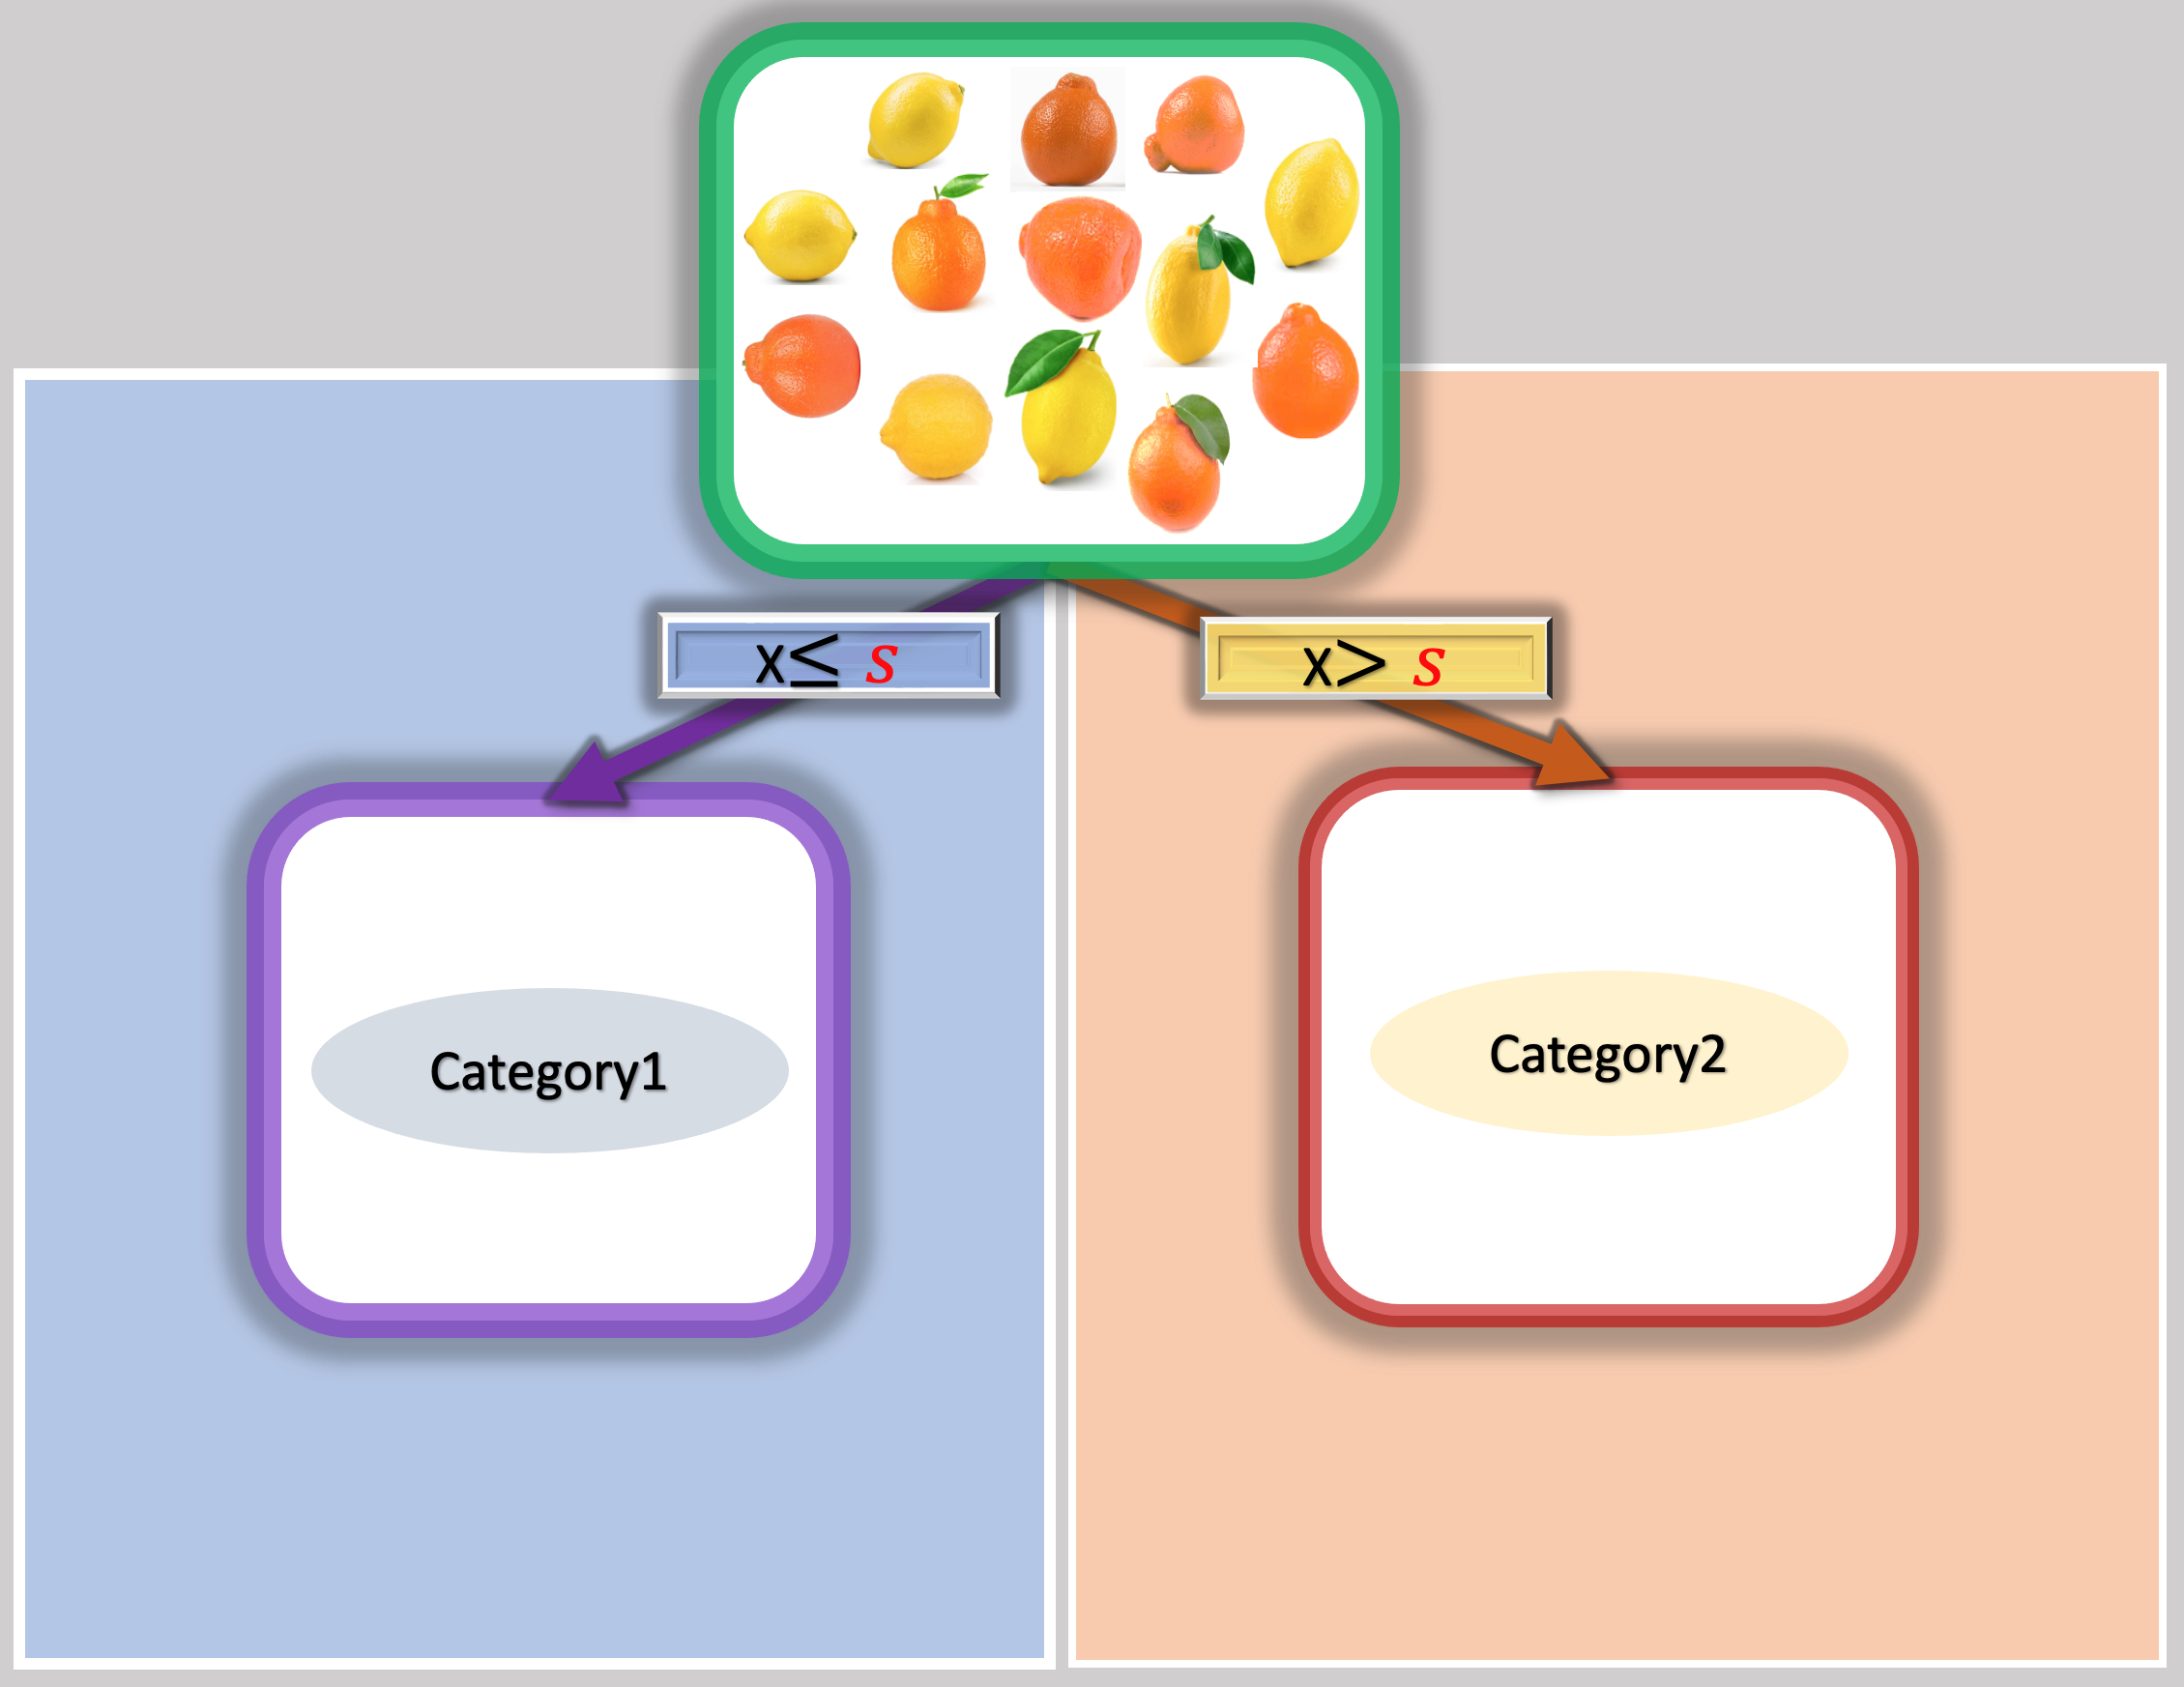
\includegraphics[scale=.23]{figs/Tree_Structure_Lemon_Orange.png}
\end{center}
%}\\
\vspace{.9in}

\end{frame}







\begin{frame}\frametitle{Classification Tree:Schematic Diagrams}
%\vspace{-.1in}
%\qBrd[4.7in]{babyblueeyes!50}{
\begin{center}
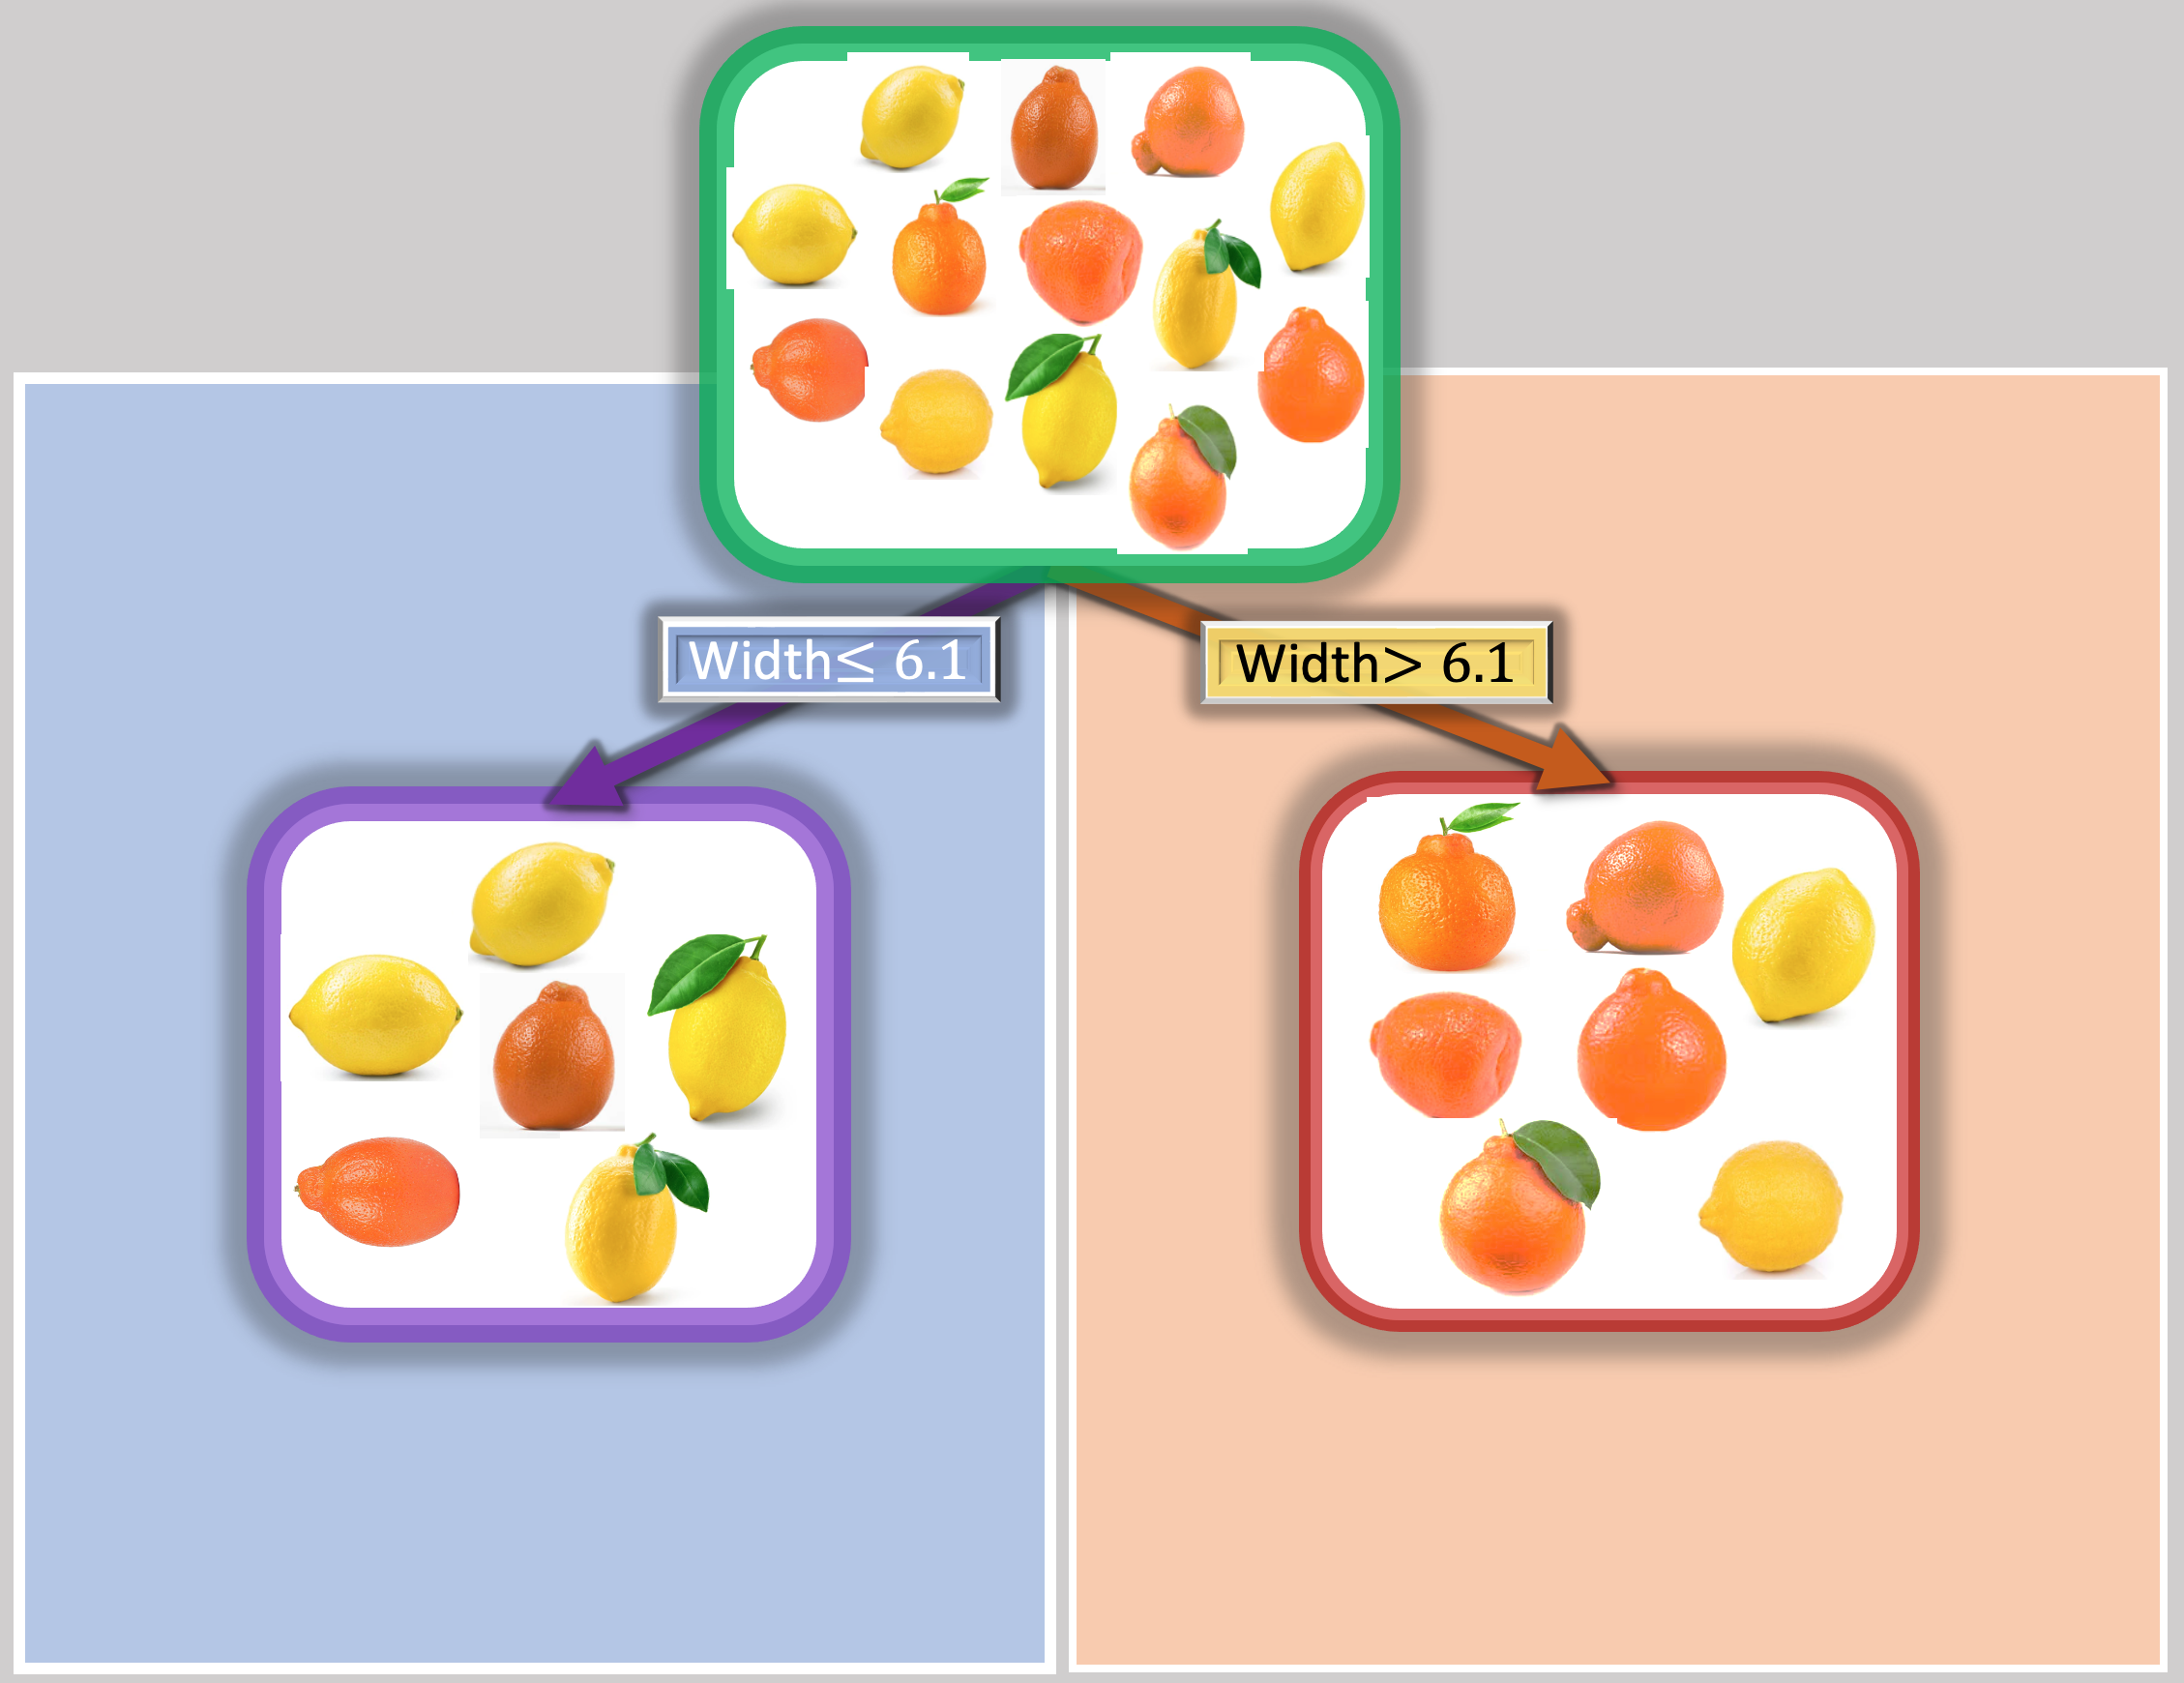
\includegraphics[scale=.23]{figs/Lemon_Orange_T1_W.png}
\end{center}
%}\\
\vspace{.9in}

\end{frame}





\begin{frame}\frametitle{Classification Tree:Schematic Diagrams}
%\vspace{-.1in}
%\qBrd[4.7in]{babyblueeyes!50}{
\begin{center}
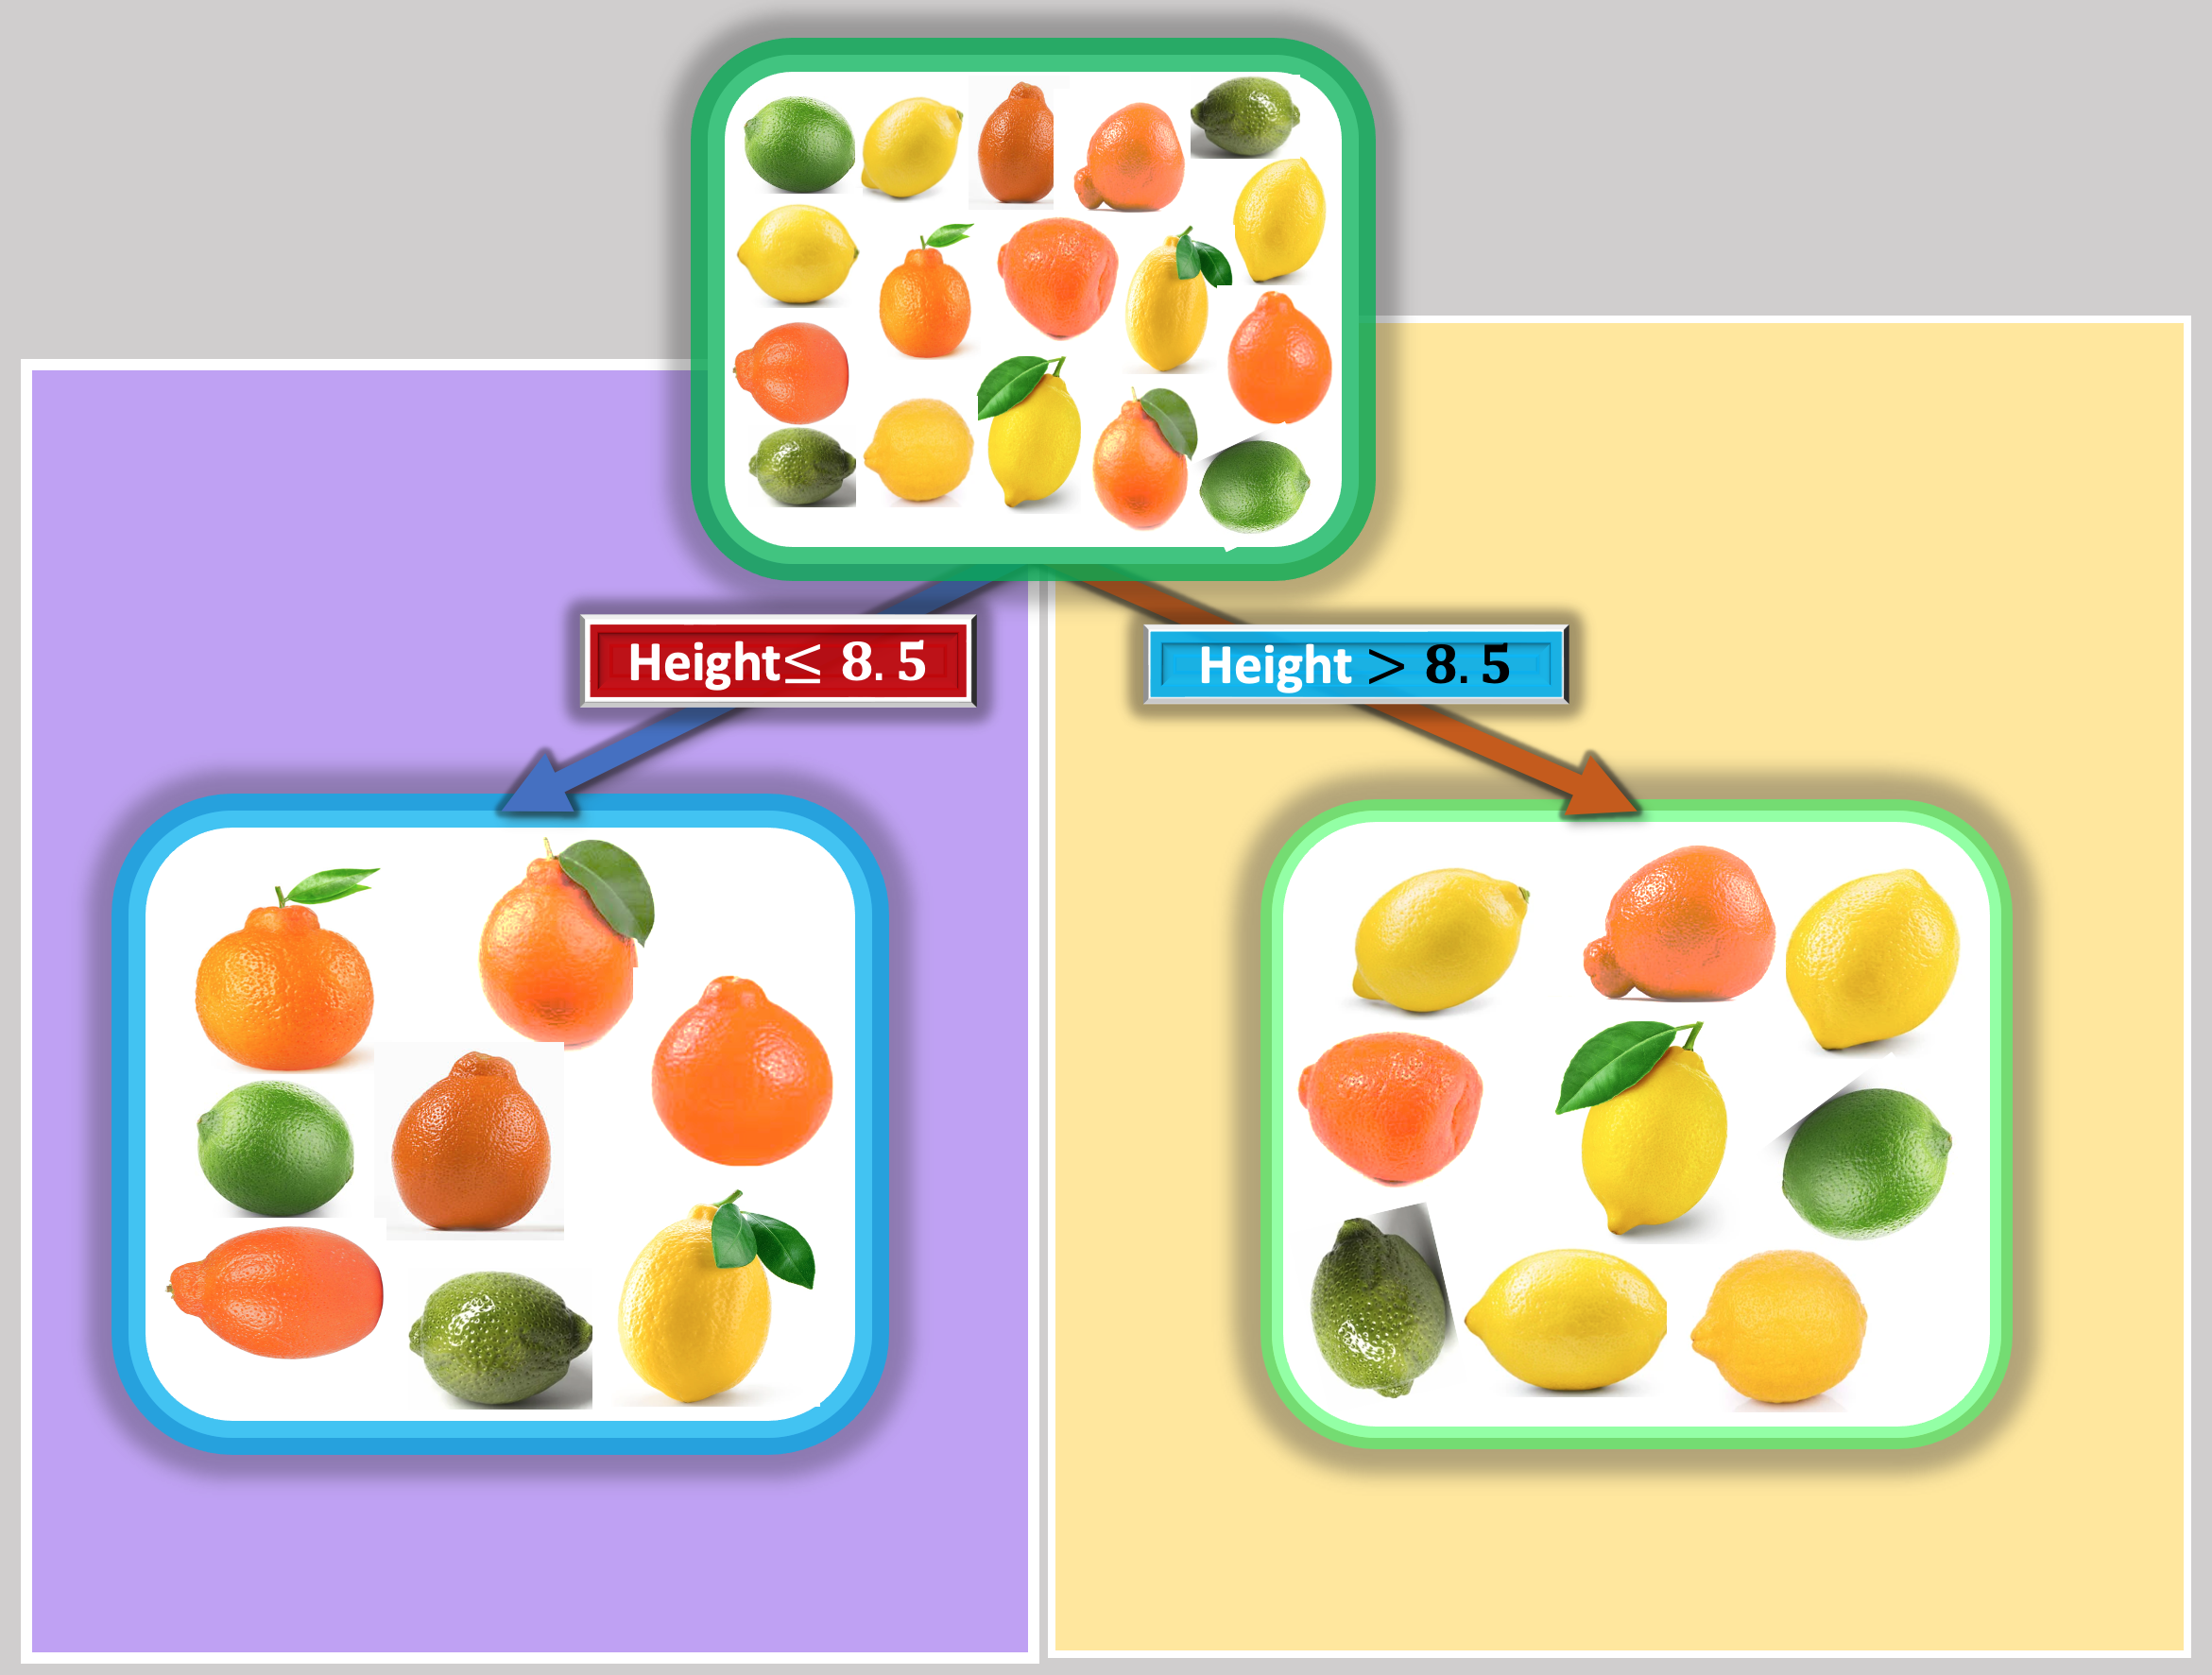
\includegraphics[scale=.23]{figs/Three_Fruits.png}
\end{center}
%}\\
\vspace{.9in}

\end{frame}




\begin{frame}\frametitle{Classification Tree:Schematic Diagrams}
%\vspace{-.1in}
%\qBrd[4.7in]{babyblueeyes!50}{
\begin{center}
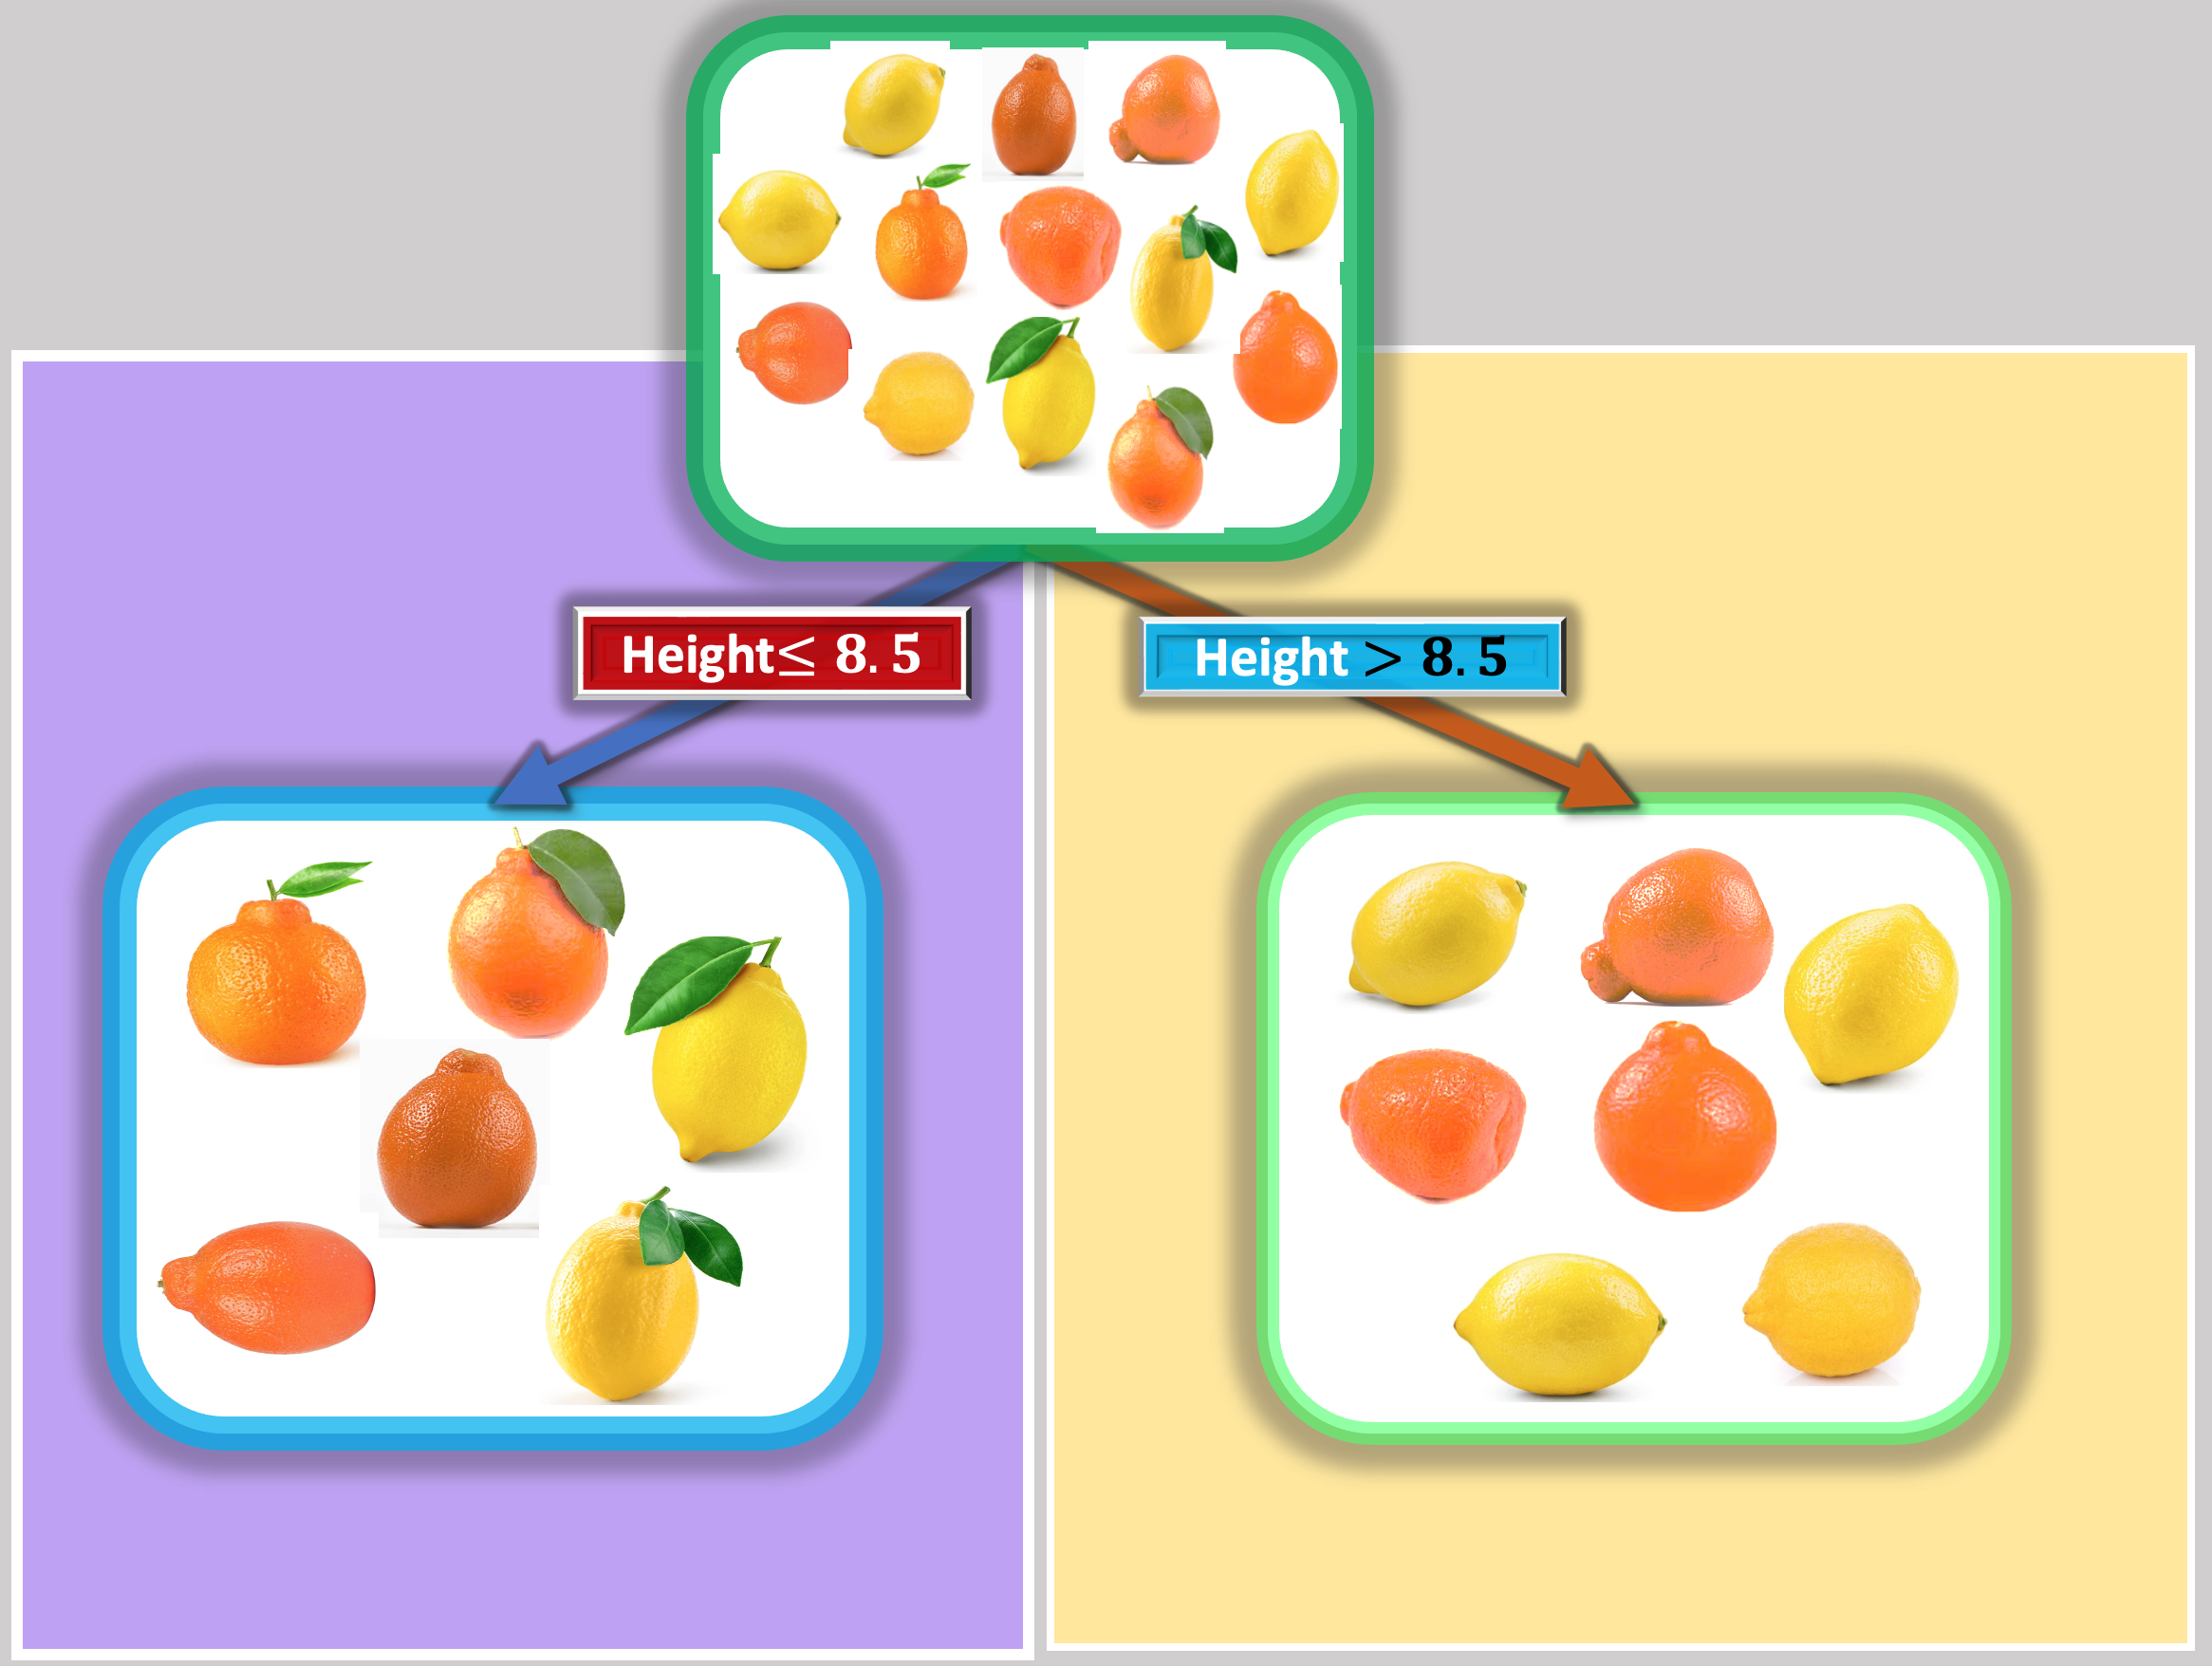
\includegraphics[scale=.25]{figs/Lemon_Orange_T2_H.png}
\end{center}
%}\\
\vspace{.9in}

\end{frame}



\subsection{Various Impurity Measures}




\begin{frame}\frametitle{Impurity Measure: Misclassification Rate}
%\vspace{-.1in}
%\qBrd[4.7in]{babyblueeyes!50}{
\begin{center}
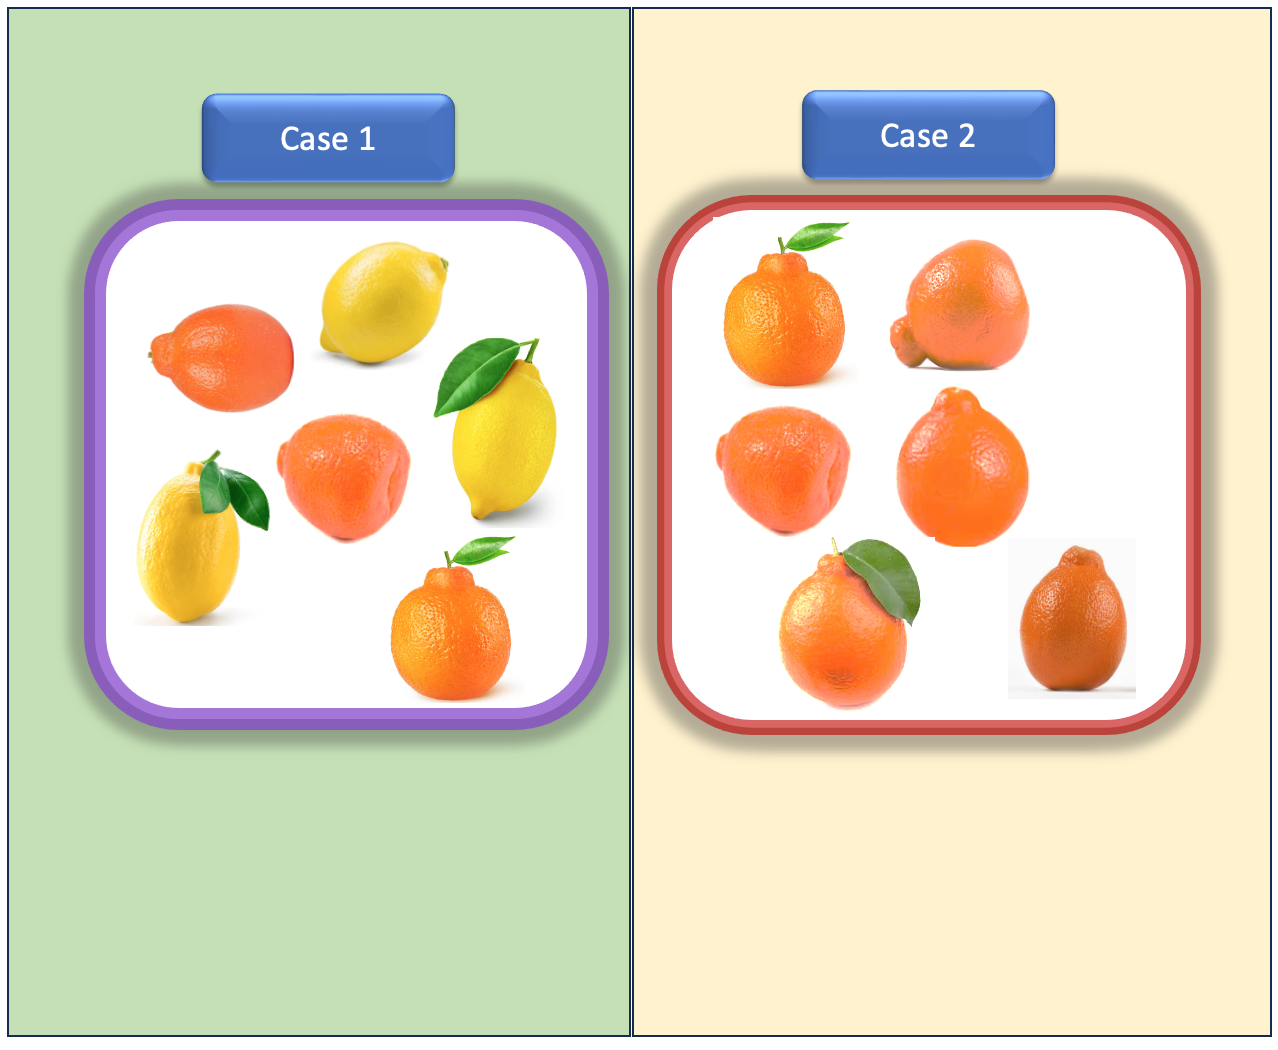
\includegraphics[scale=.42]{figs/Impurity.png}
\end{center}
%}\\
\vspace{.9in}

\end{frame}



\begin{frame}
\begin{center}
$\Row{{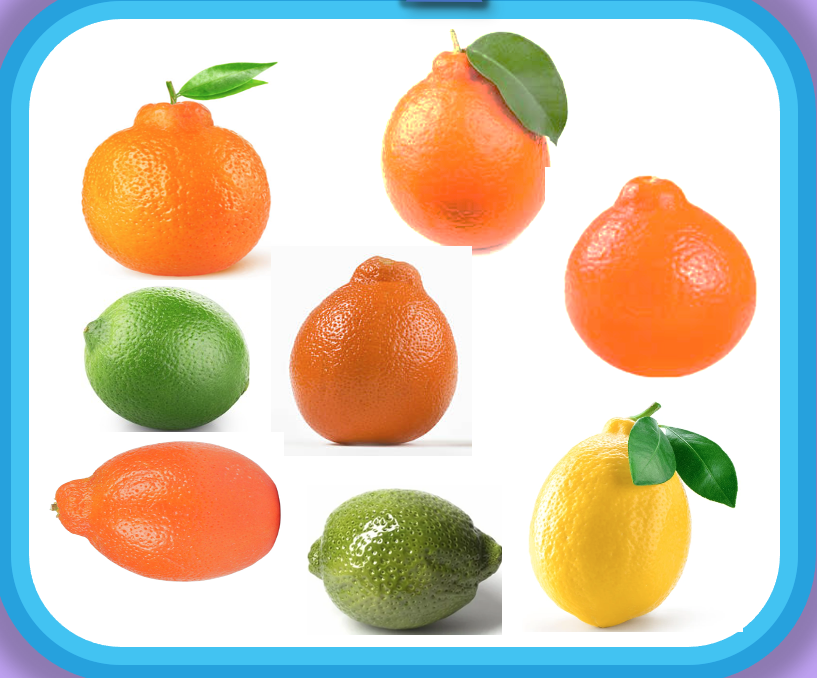
\includegraphics[scale=.2]{figs/Three_Fruits1.png}},{\RowVec{n_1=4,n_2=1,n_3=2}}}$
\end{center}
\qBrd[4.5in]{babyblueeyes!50}{
\begin{enumerate}
\qBrd[2in]{airforceblue!50}{
\item[\sqBullet{bluebell}]  $\left( \Row{n_1=20, n_2=15, n_3=5} \right)$
\vspace{.3in}
}
\qBrd[2in]{babyblue!50}{
\item[\sqBullet{babyblue}]  $\MakeVec{p}= \left( \Row{.3, .6, .1} \right)$
\vspace{.3in}
}
\qBrd[2in]{airforceblue!50}{
\item[\sqBullet{bluebell}]  $\MakeVec{p}= \left( \Row{\frac{1}{3},\frac{1}{3}, \frac{1}{3}} \right)$
\vspace{.3in}
}
\qBrd[2in]{airforceblue!50}{
\item[\sqBullet{bluebell}]  $\MakeVec{p}= \left( \Row{1,0, 0} \right)$
\vspace{.3in}
}
\end{enumerate}
}\\
\vspace{.2in}

\end{frame}



\begin{frame}\frametitle{Impurity Measure: Gini Index}
\qBrd[4.5in]{babyblueeyes!50}{
\begin{enumerate}
\qBrd[2in]{airforceblue!50}{
\item[\sqBullet{bluebell}]  $\left( \Row{n_1=20, n_2=15, n_3=5} \right)$
\vspace{.3in}
}
\qBrd[2in]{babyblue!50}{
\item[\sqBullet{babyblue}]  $\MakeVec{p}= \left( \Row{.3, .6, .1} \right)$
\vspace{.3in}
}
\qBrd[2in]{airforceblue!50}{
\item[\sqBullet{bluebell}]  $\MakeVec{p}= \left( \Row{\frac{1}{3},\frac{1}{3}, \frac{1}{3}} \right)$
\vspace{.3in}
}
\qBrd[2in]{airforceblue!50}{
\item[\sqBullet{bluebell}]  $\MakeVec{p}= \left( \Row{1,0, 0} \right)$
\vspace{.3in}
}
\end{enumerate}
}\\
\vspace{.2in}

\end{frame}





\begin{frame}\frametitle{Impurity Measure: Entropy Measure}
\qBrd[4.5in]{babyblueeyes!50}{
\begin{enumerate}
\qBrd[2in]{airforceblue!50}{
\item[\sqBullet{bluebell}]  $\left( \Row{n_1=20, n_2=15, n_3=5} \right)$
\vspace{.3in}
}
\qBrd[2in]{babyblue!50}{
\item[\sqBullet{babyblue}]  $\MakeVec{p}= \left( \Row{.3, .6, .1} \right)$
\vspace{.3in}
}
\qBrd[2in]{airforceblue!50}{
\item[\sqBullet{bluebell}]  $\MakeVec{p}= \left( \Row{\frac{1}{3},\frac{1}{3}, \frac{1}{3}} \right)$
\vspace{.3in}
}
\qBrd[2in]{airforceblue!50}{
\item[\sqBullet{bluebell}]  $\MakeVec{p}= \left( \Row{1,0, 0} \right)$
\vspace{.3in}
}
\end{enumerate}
}\\
\vspace{.2in}

\end{frame}

\begin{frame}\frametitle{Classification Tree: Schematic Diagrams}
%\vspace{-.1in}
%\qBrd[4.7in]{babyblueeyes!50}{
\begin{center}
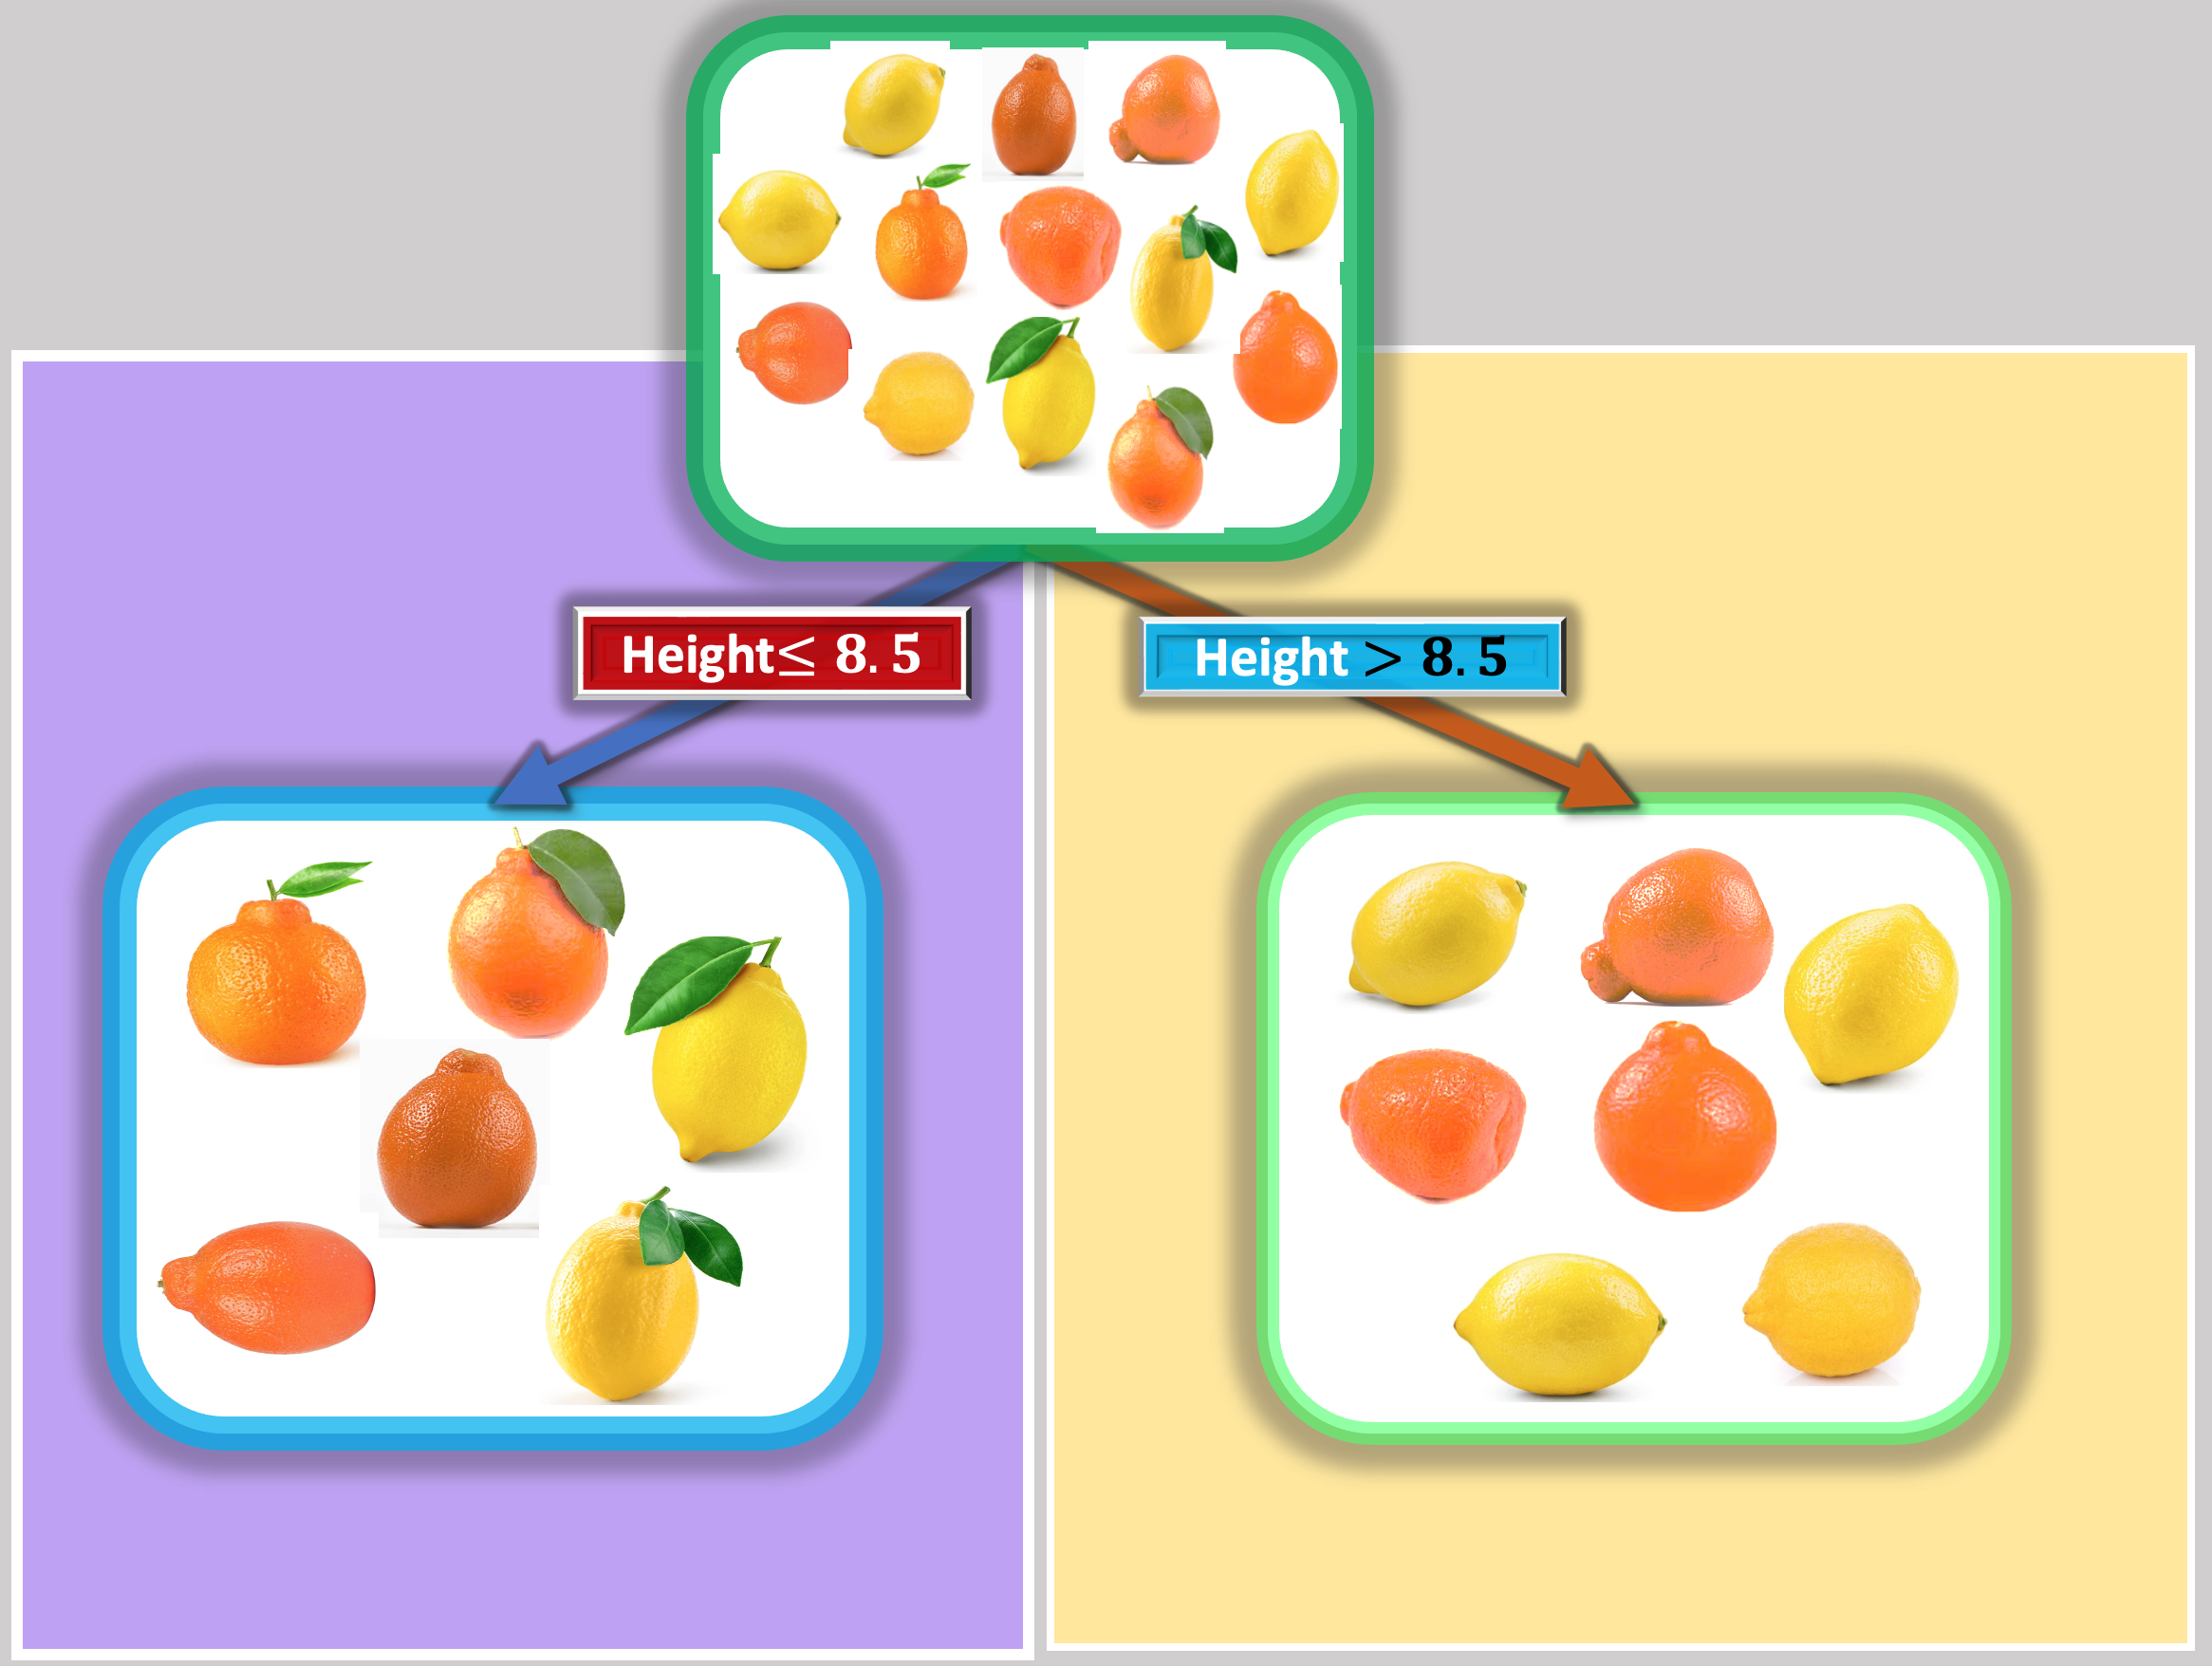
\includegraphics[scale=.25]{figs/Lemon_Orange_T2_H.png}
\end{center}
%}\\
\vspace{.9in}

\end{frame}



\begin{frame}{}
\qbx[4.5in]{slateblue!40}{\sqBullet{slateblue} If we define model prediction based on the most commonly occurring class of training  observations in a given region, the \HLTY{\text{classification error rate}} is the proportion of the training observations that do not belong to the most common class :\begin{center}
\qBrd[3in]{rose!20}{$$\HLTY{\text{classification error rate}}=\HLTW{ 1-\max\limits_{k}\hat{p}_{m,k}} \vspace{-.1in}$$}
\end{center}}

\vspace{1.7in}
\end{frame}




\begin{frame}{}
\qbx[4.5in]{babyblueeyes!40}{\sqBullet{babyblueeyes} If we define model prediction based on the most commonly occurring class of training  observations in a given region, the \HLTY{\text{Gini index}} measures the impurity using the following formula
\begin{center}
\qBrd[3in]{rose!20}{$$\HLTY{\text{G}}=\HLTW{\displaystyle  \sum_{k=1}^{K}\hat{p}_{m,k} \left(1-\hat{p}_{m,k}\right)} \vspace{-.1in}$$}
\end{center}}
Gini index is a measure of node purity - a small value indicates that a
node contains predominantly observations from a single class.
\vspace{1.7in}
\end{frame}





\begin{frame}{}
\qbx[4.5in]{rose!40}{\sqBullet{rose} If we define model prediction based on the most commonly occurring class of training  observations in a given region, the \HLTY{\text{cross-entropy}} measures the impurity using the following formula
\begin{center}
\qBrd[3in]{rose!20}{$$\HLTY{\text{D}}=\HLTW{\displaystyle - \sum_{k=1}^{K}\hat{p}_{m,k} \log \left(\hat{p}_{m,k}\right)} \vspace{-.1in}$$}
\end{center}}
\vspace{1.7in}
\end{frame}




{
 \setbeamercolor{background canvas}{bg=}
%
\includepdf[pages={1}, scale=1, trim=1mm 5mm 11mm 5mm]{STAT380-Unit2.pdf}
\includepdf[pages={95-96}, scale=1]{STAT380-Unit3.pdf}
}


\subsection{Classification Tree Algorithm}

\begin{frame}\frametitle{Classification Tree:Schematic Diagrams}
\vspace{-.2in}
\qBrd[4.7in]{babyblueeyes!50}{
\begin{center}
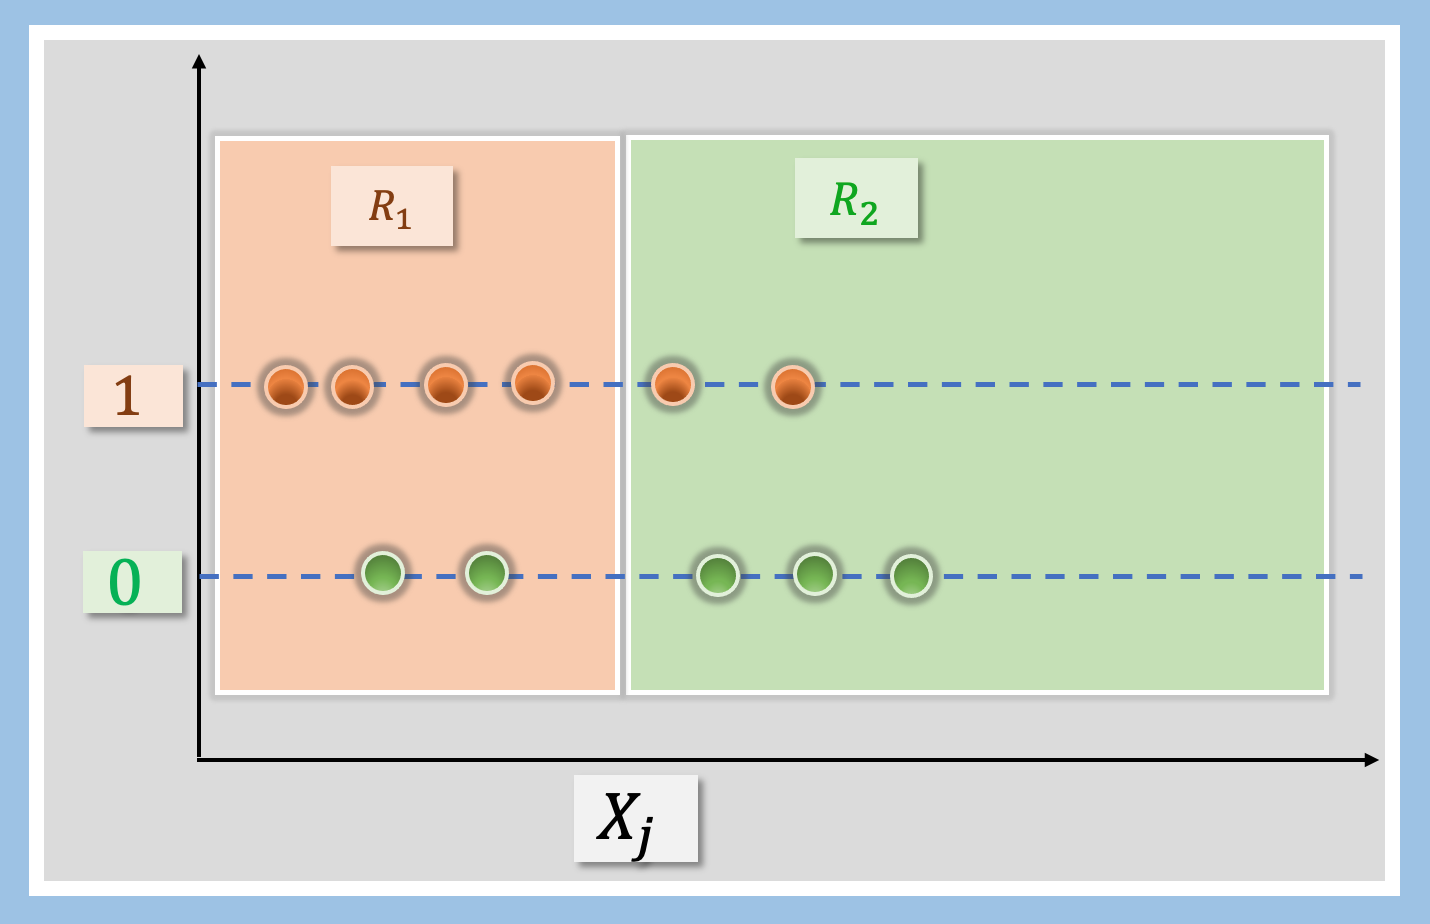
\includegraphics[scale=.3]{figs/Decission_Tree1.png}
\end{center}
}\\
\vspace{.9in}

\end{frame}





\begin{frame}\frametitle{Classification Tree:Schematic Diagrams}
\vspace{-.5in}
\qBrd[4.7in]{babyblueeyes!50}{
\begin{center}
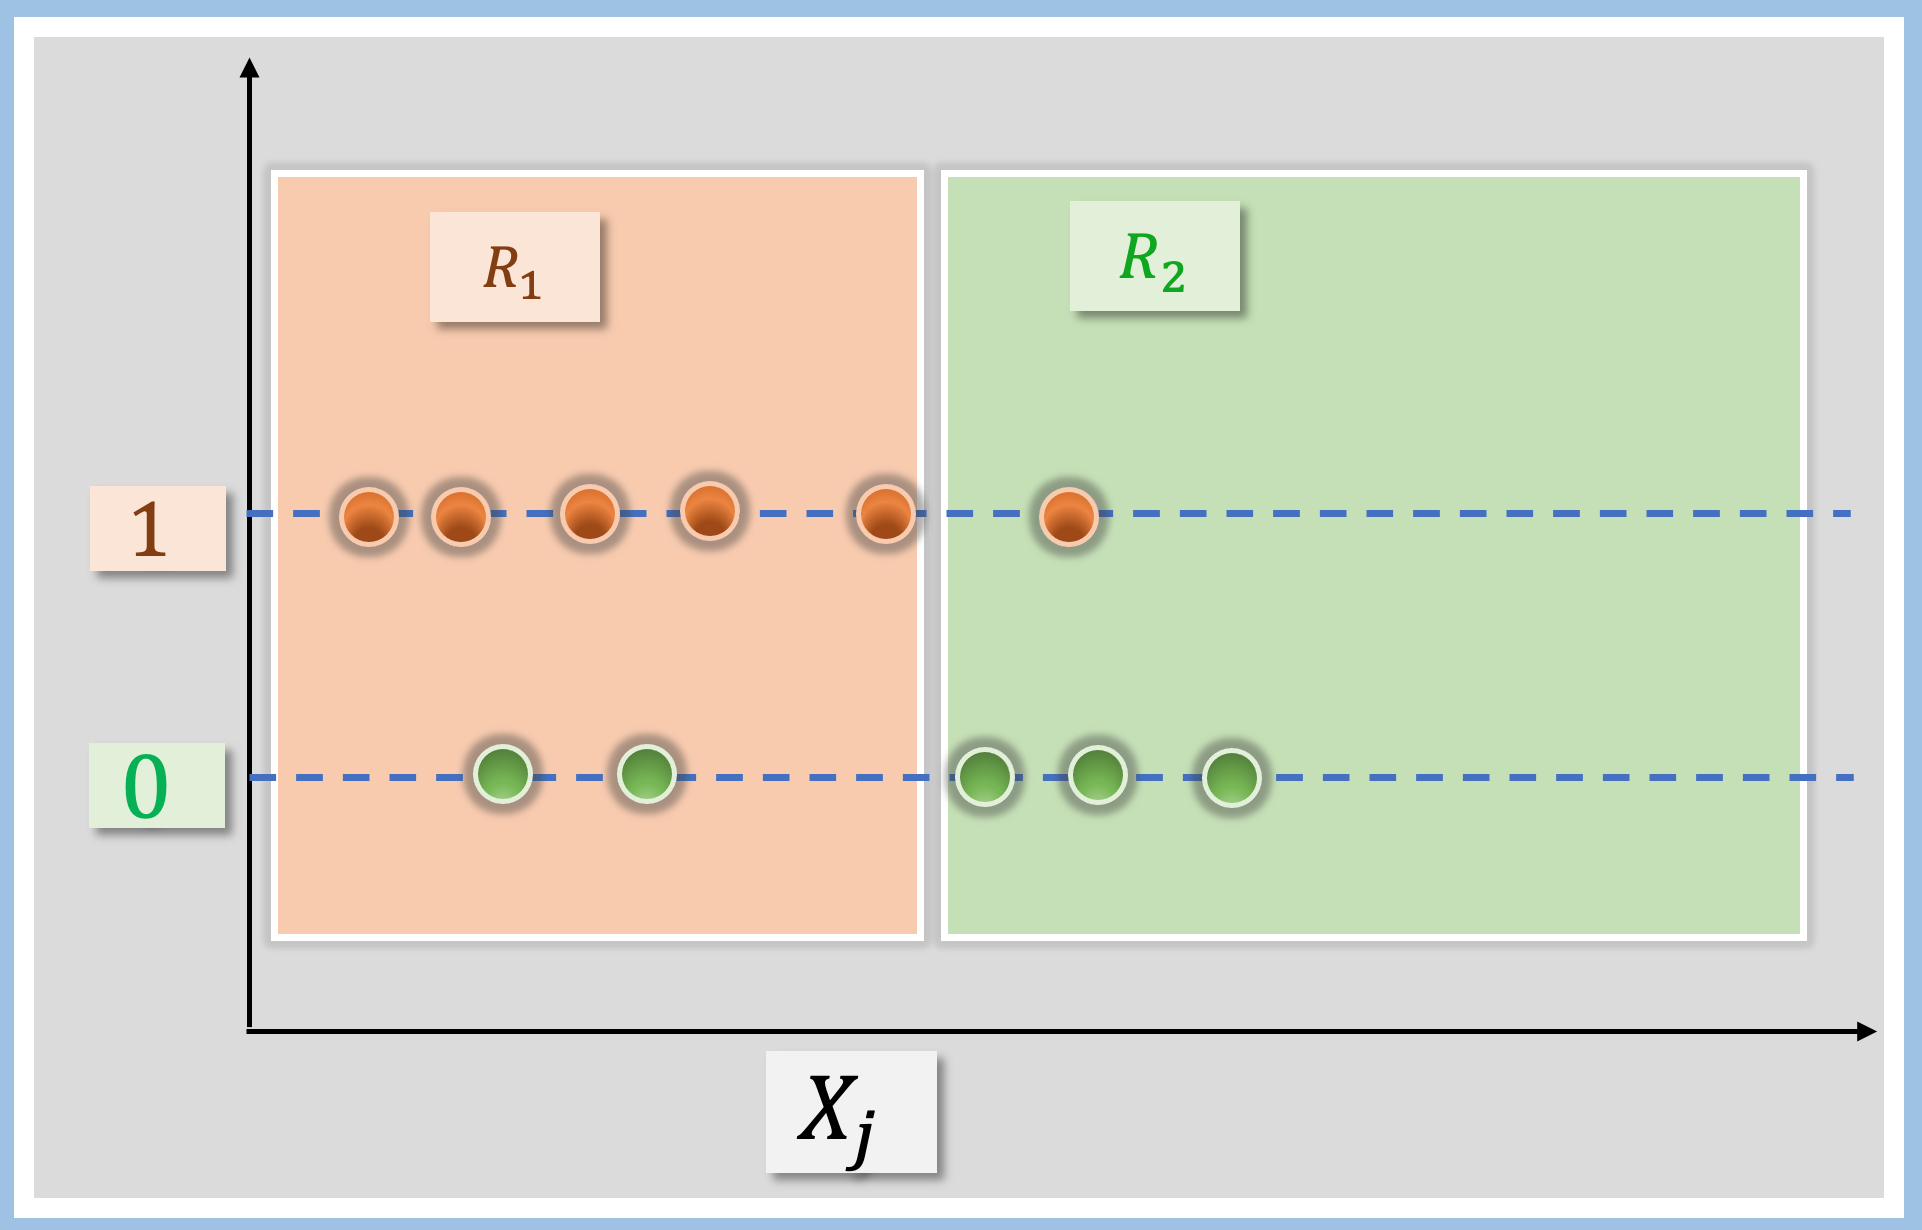
\includegraphics[scale=.23]{figs/Decission_Tree2.png}
\end{center}
}\\
\vspace{.2in}

\end{frame}






\begin{frame}
\qBrd[4.5in]{babyblueeyes!50}{
\begin{center}
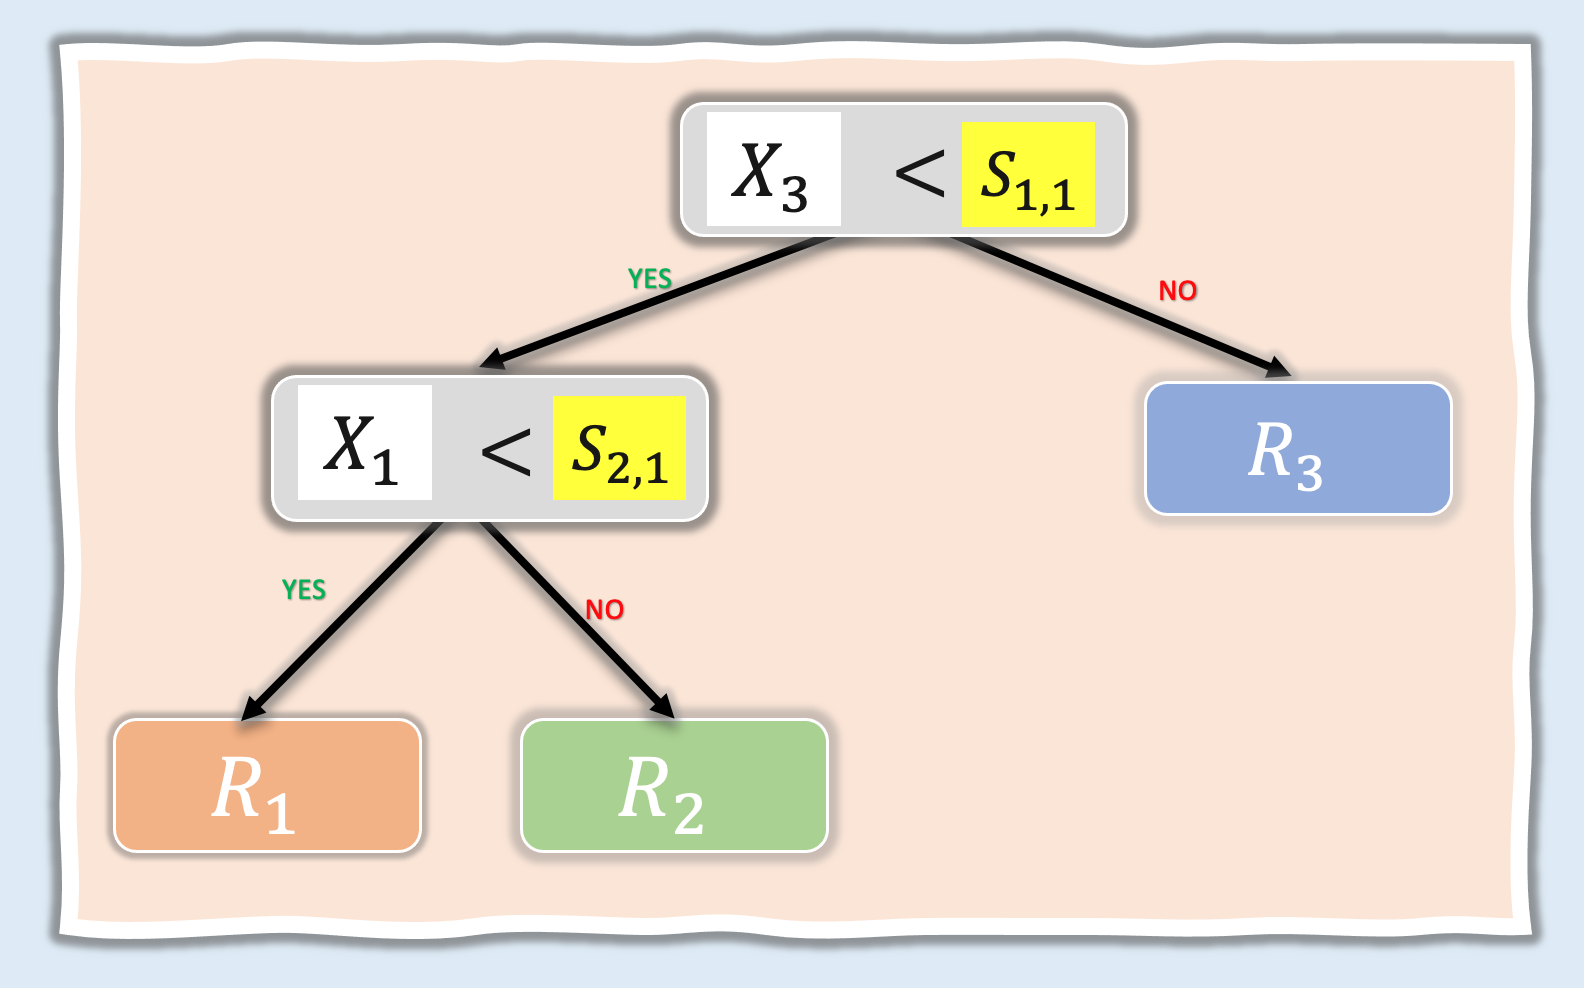
\includegraphics[scale=.32]{figs/RegressionTreeDiagram.png}
\end{center}
%\vspace{.1in}
\begin{enumerate}
\qBrd[4in]{airforceblue!50}{
\item[\sqBullet{bluebell}] How do we decide which varibale to select while creating the binary split? i.e. which one among  $\HLTW{\{X_1, \ldots X_p\}}$
}
\qBrd[4in]{babyblue!50}{
\item[\sqBullet{babyblue}]  How do we select the cut off $\HLTY{S}$?
}
\end{enumerate}
}\\
\vspace{.2in}

\end{frame}






\begin{frame}
\vspace{-.1in}
\qBrd[4.5in]{babyblueeyes!50}{
\begin{center}
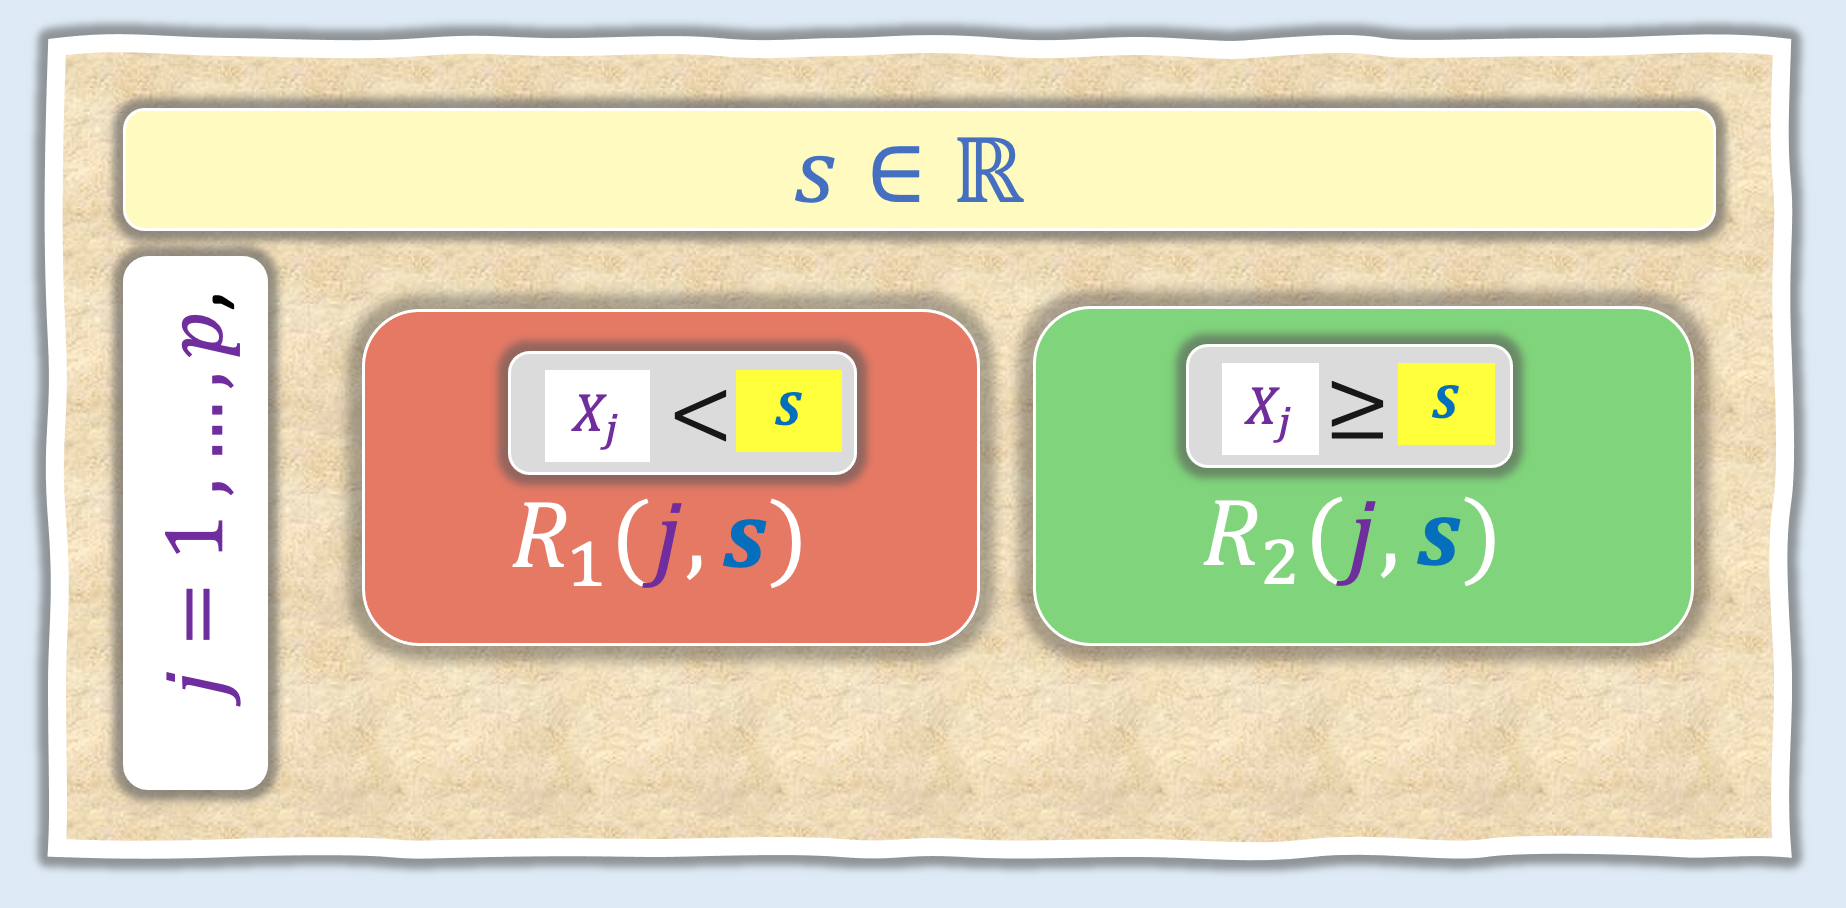
\includegraphics[scale=.3]{figs/R1_R2.png}
\end{center}
\vspace{-.15in}
}\\
\vspace{-.18in}
\begin{center}
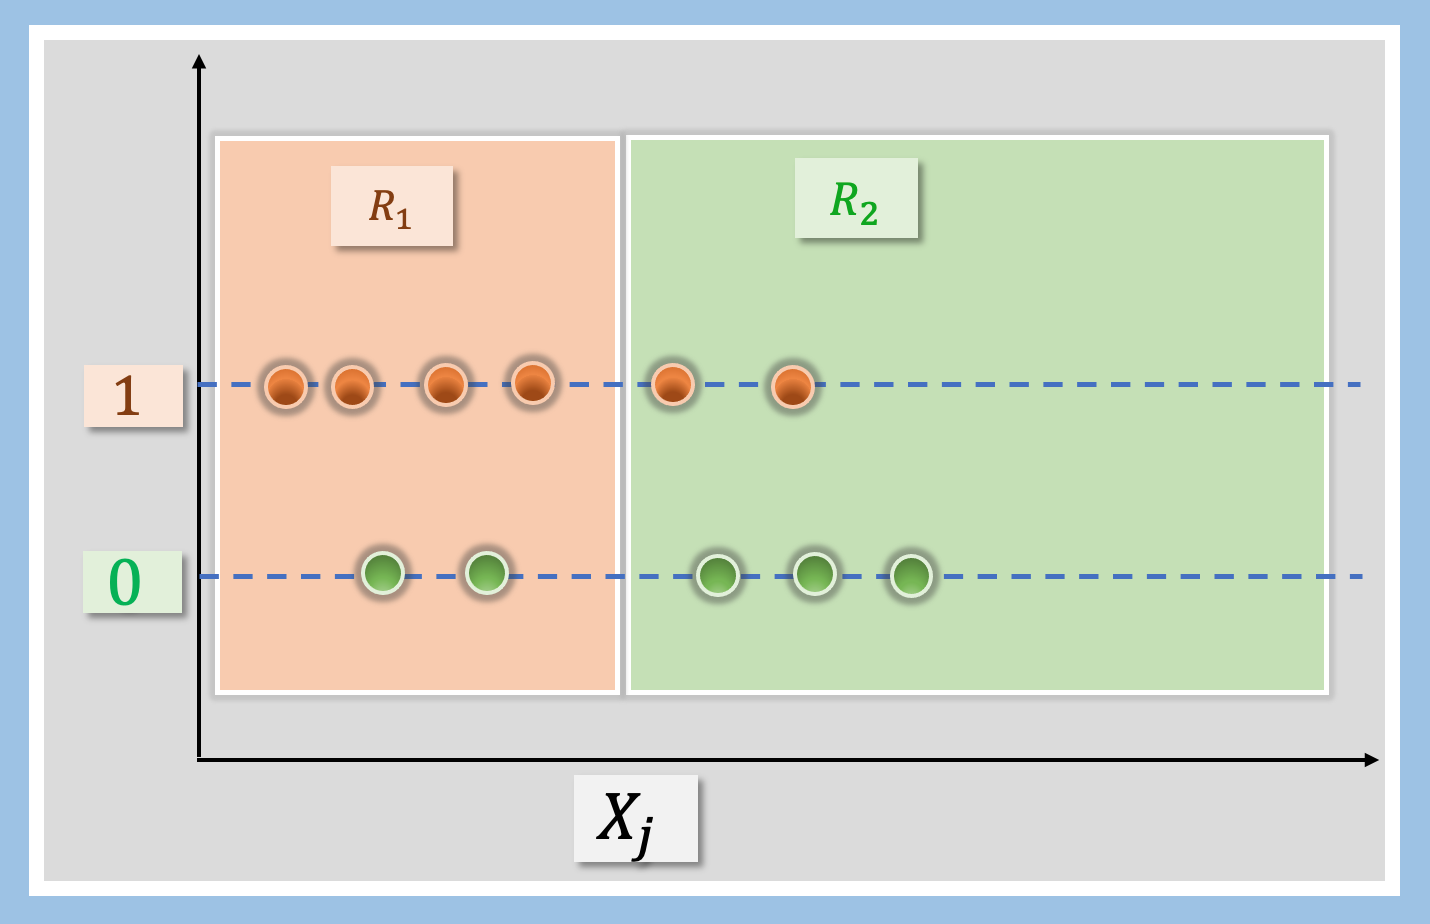
\includegraphics[scale=.22]{figs/Decission_Tree1.png}
\end{center}
\vspace{-.15in}
\end{frame}


\newcommand{\impurity}{{\mathcal{I}}}
\begin{frame}
%\qBrd[4.7in]{babyblueeyes!50}{
%\begin{center}
%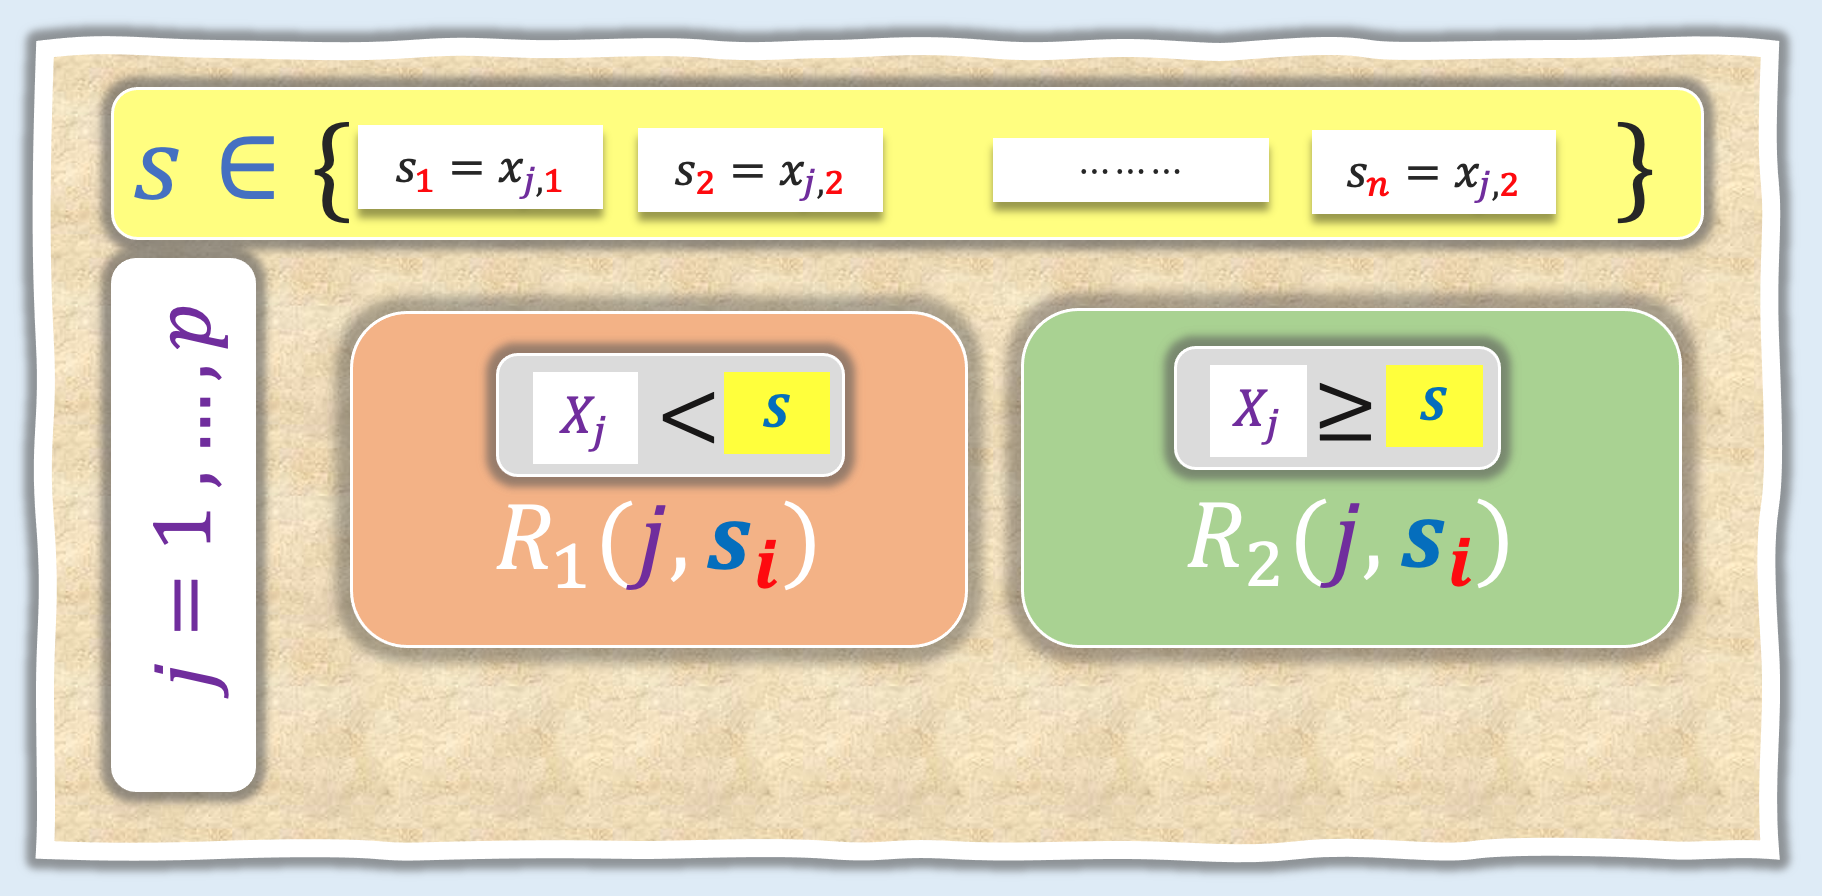
\includegraphics[scale=.15]{figs/R1_R2_s.png}
%\end{center}
%%\vspace{.1in}
%}\\
\qBrd[4.7in]{airforceblue!50}{
Let the dataset $\mathcal{D}$ is partitioned into two parts $R_1:=\{X_j\leq s\}$, and $R_2:=\{X_j> s\}$
\begin{enumerate}
\item  $\HLTW{ \mathcal{D}:=R_1\cup R_2}$ denotes the entire dataset.  (training data set) 
\item $\HLTW{\vert  \mathcal{D}\vert = n}$, sample size. 
\item $\HLTW{\vert  R_1 \vert = n_1}$, number sof amples in $R_1$.
\item $\HLTW{\vert  R_2 \vert = n_2}$, number sof amples in $R_2$.
\item$\HLTW{n_1+ n_2=n}$
\item $\HLTY{\impurity(\mathcal{D})}, \HLTEQ[applegreen!40]{\impurity(R_1)}, \HLTEQ[celadon!40]{\impurity( R_2)}$ denotes an {\it impurity measure } for $\HLTY{\mathcal{D}}$, $R_1$,  and $R_2$, respectively. 
\end{enumerate}
}

\qBrd[4.7in]{airforceblue!50}{
The impurity reduction/ information gain is defined to be.
$$\DBX{\HLTW{  \Delta\impurity(j , s_i)}}:=  {\HLTW{\HLTY{ \impurity(\mathcal{D} )  } } - \left\{ \HLTW{ \displaystyle   \frac{n_1 }{n_1+n_2}\HLTEQ[applegreen!40]{\impurity( R_1)} +  \frac{n_2}{n_1+n_2}\HLTEQ[celadon!40]{\impurity( R_2)}  }\right\}} $$
}

\end{frame}




%
%
%\begin{frame}
%\qBrd[4.6in]{babyblueeyes!50}{
%\begin{center}
%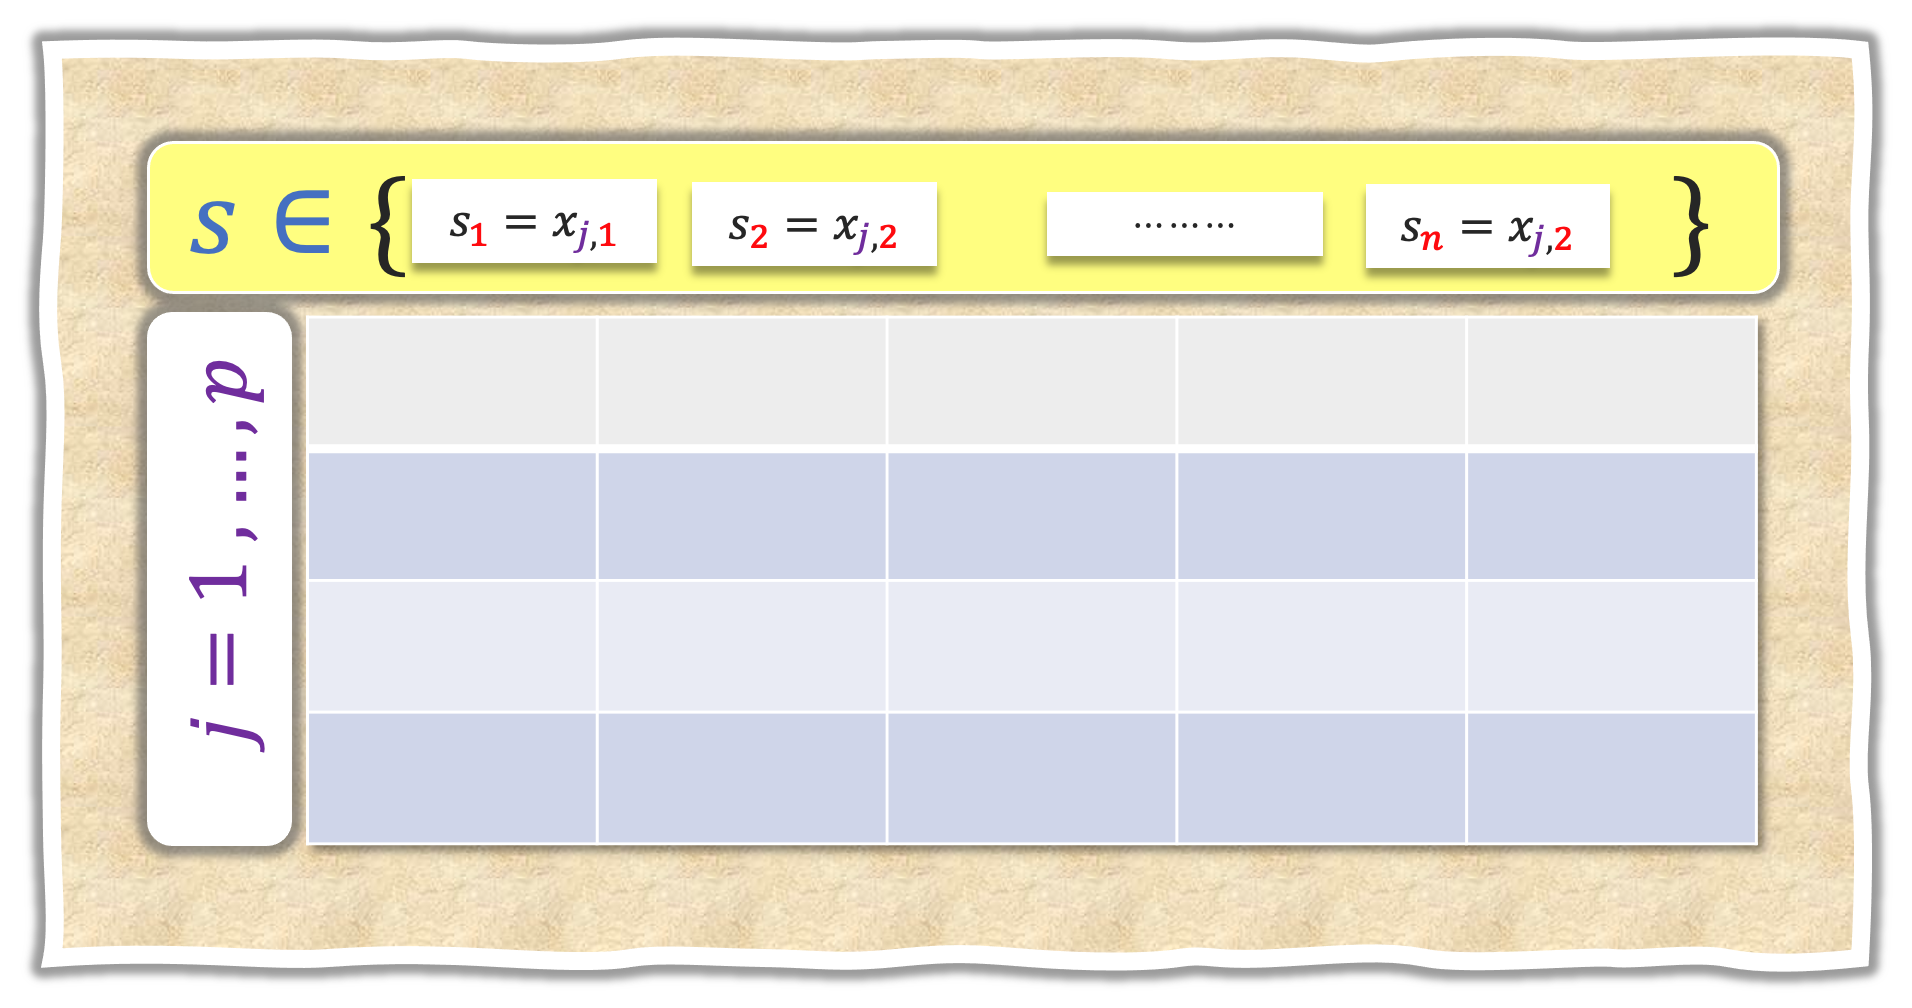
\includegraphics[scale=.35]{figs/R1_R2_table.png}
%\end{center}
%%\vspace{.1in}
%}\\
%\vspace{.7in}
%
%\end{frame}
%



\begin{frame}
\qBrd[4.7in]{bubblegum!50}{
\begin{center}
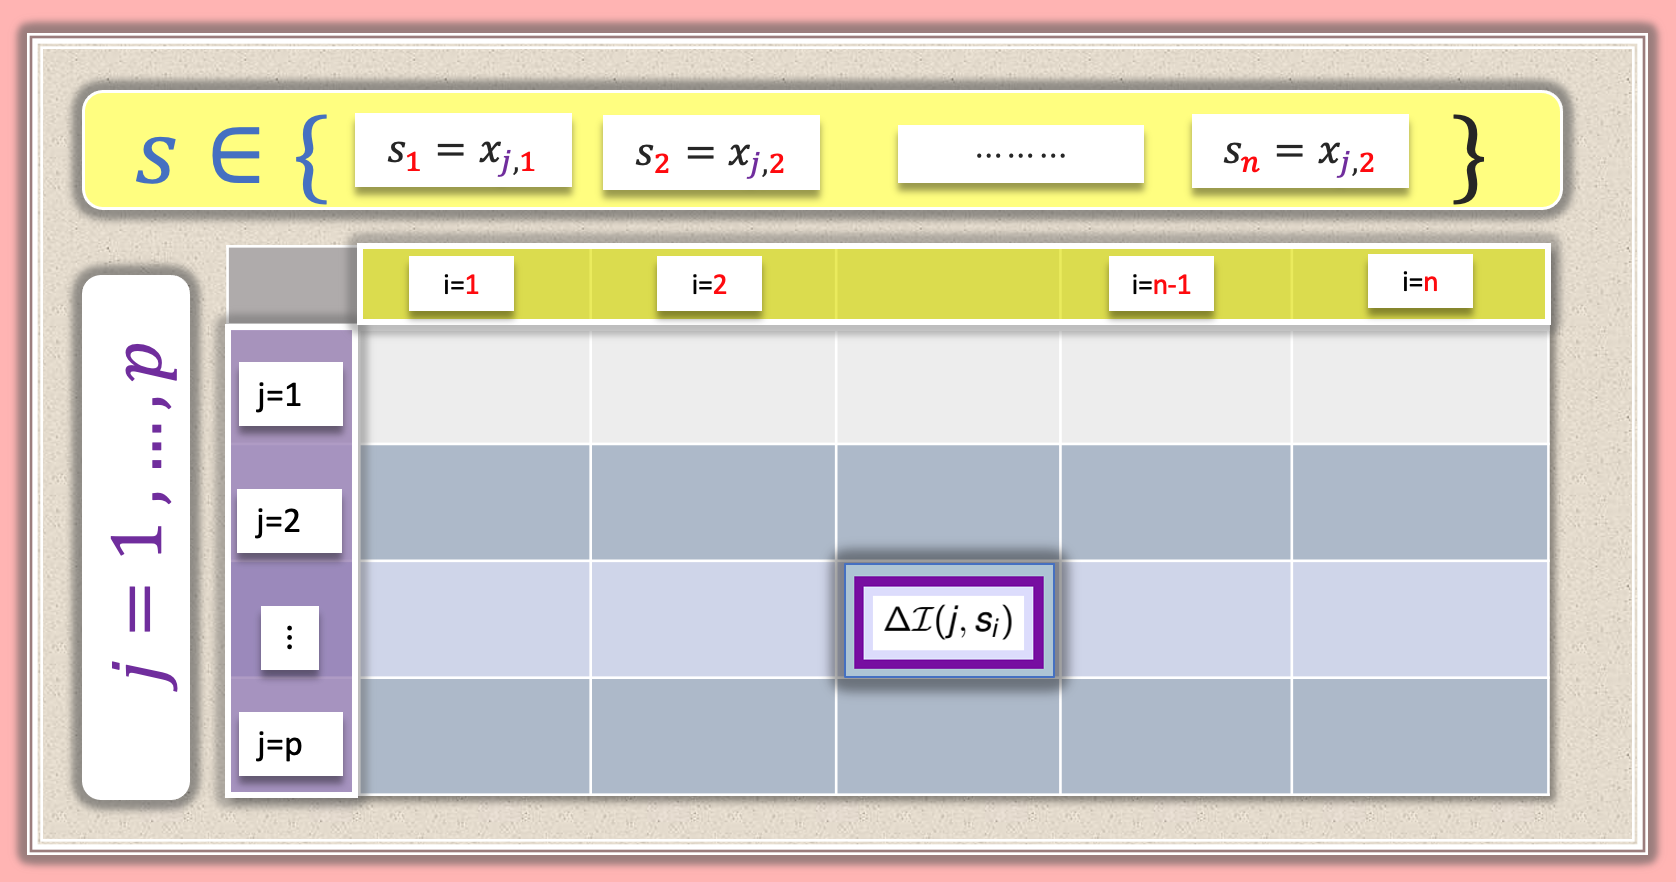
\includegraphics[scale=.35]{figs/R1_R2_table1_impurity.png}\\
%\vspace{.1in}
%\begin{enumerate}
\vspace{.2in}
\qBrd[4in]{coralpink!70}{
$$\HLTW{ \displaystyle (j_{_{_\text{opt}}},   i_{_{_\text{opt}}} )} := \HLTW{ \displaystyle\argmax_{j\in \{1, \ldots p\}, i\in \{1, \ldots , n \}}  \DBX{\HLTW{  \Delta\impurity(j , s_i)}}}$$
}
\end{center}
%\qBrd[4in]{babyblue!50}{
%\item[\sqBullet{babyblue}]  A
%}
%\end{enumerate}
}\\
\vspace{1in}


\end{frame}





\begin{frame}\frametitle{Classification Tree:Schematic Diagrams}
\vspace{-.2in}
$\Row{{\qBrd[2.2in]{darklavender!40}{
\begin{center}
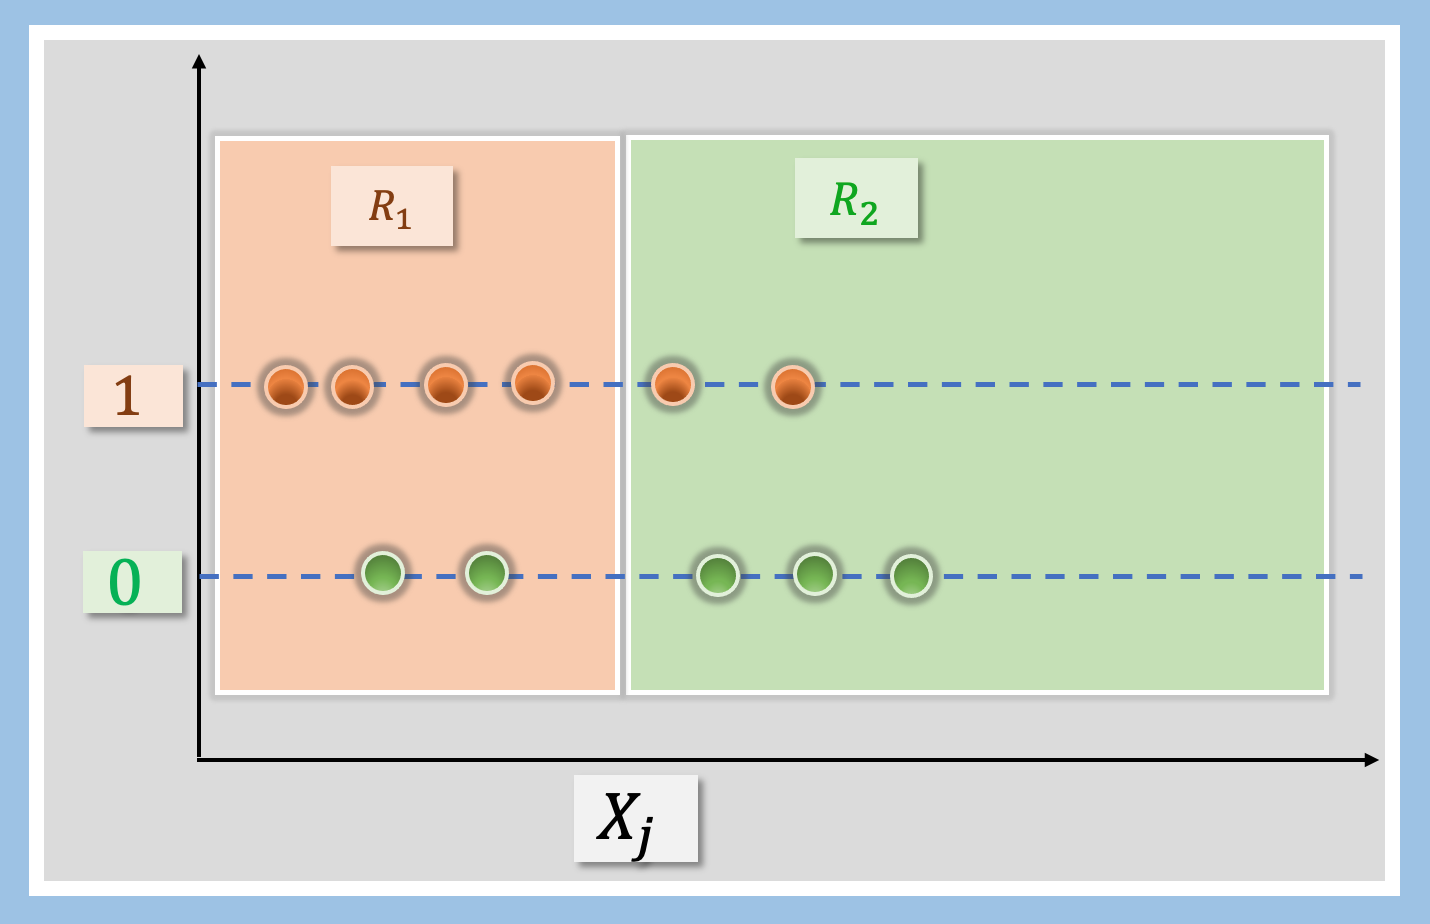
\includegraphics[scale=.2]{figs/Decission_Tree1.png}
\end{center}
\vspace{1.5in}
}}, 
{\qBrd[2.2in]{cadmiumorange!40}{
\begin{center}
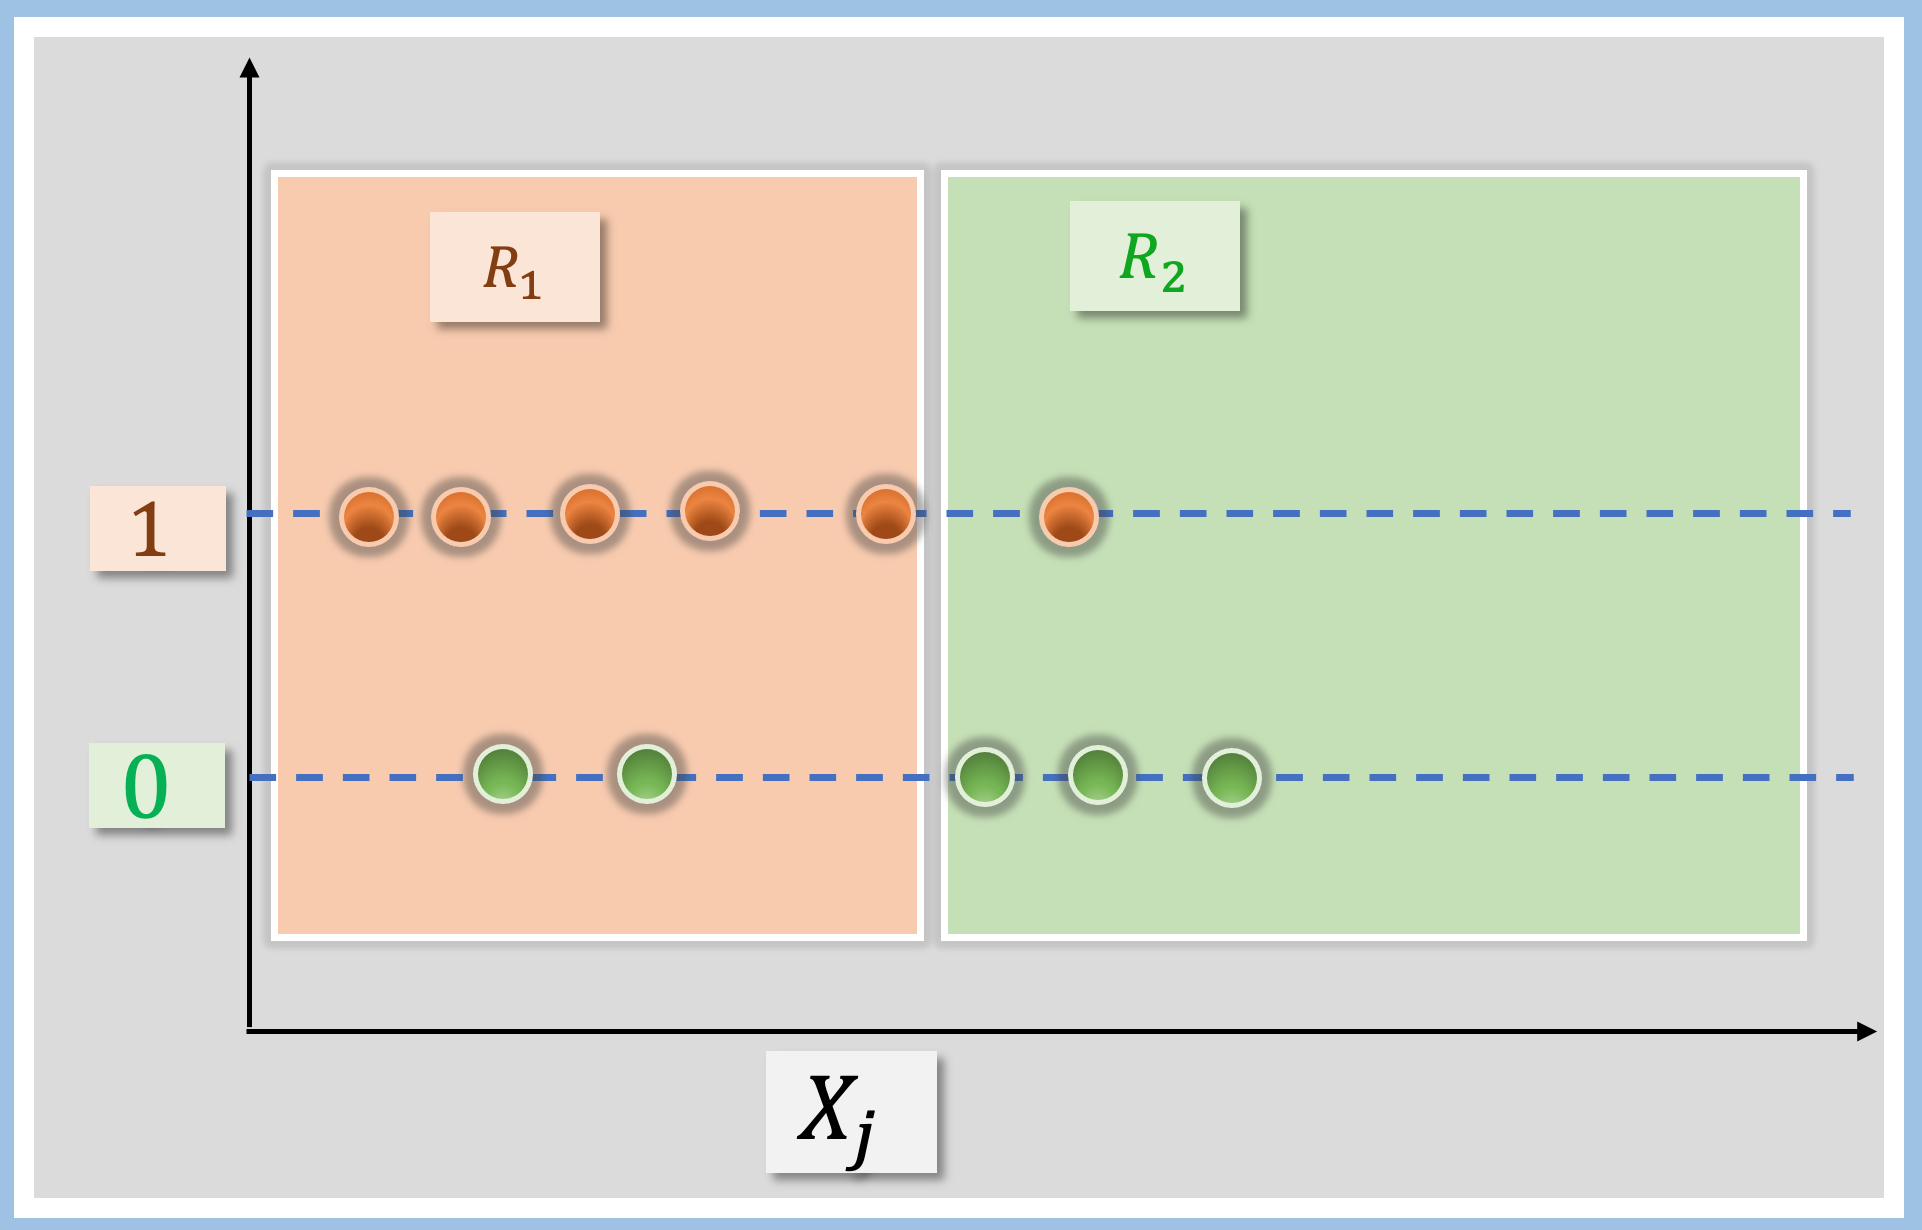
\includegraphics[scale=.15]{figs/Decission_Tree2.png},
\end{center}
\vspace{1.5in}
}}}$


\end{frame}

\subsection{An Example}


\begin{frame}
\qBrd[4.7in]{babyblueeyes!50}{
\begin{center}
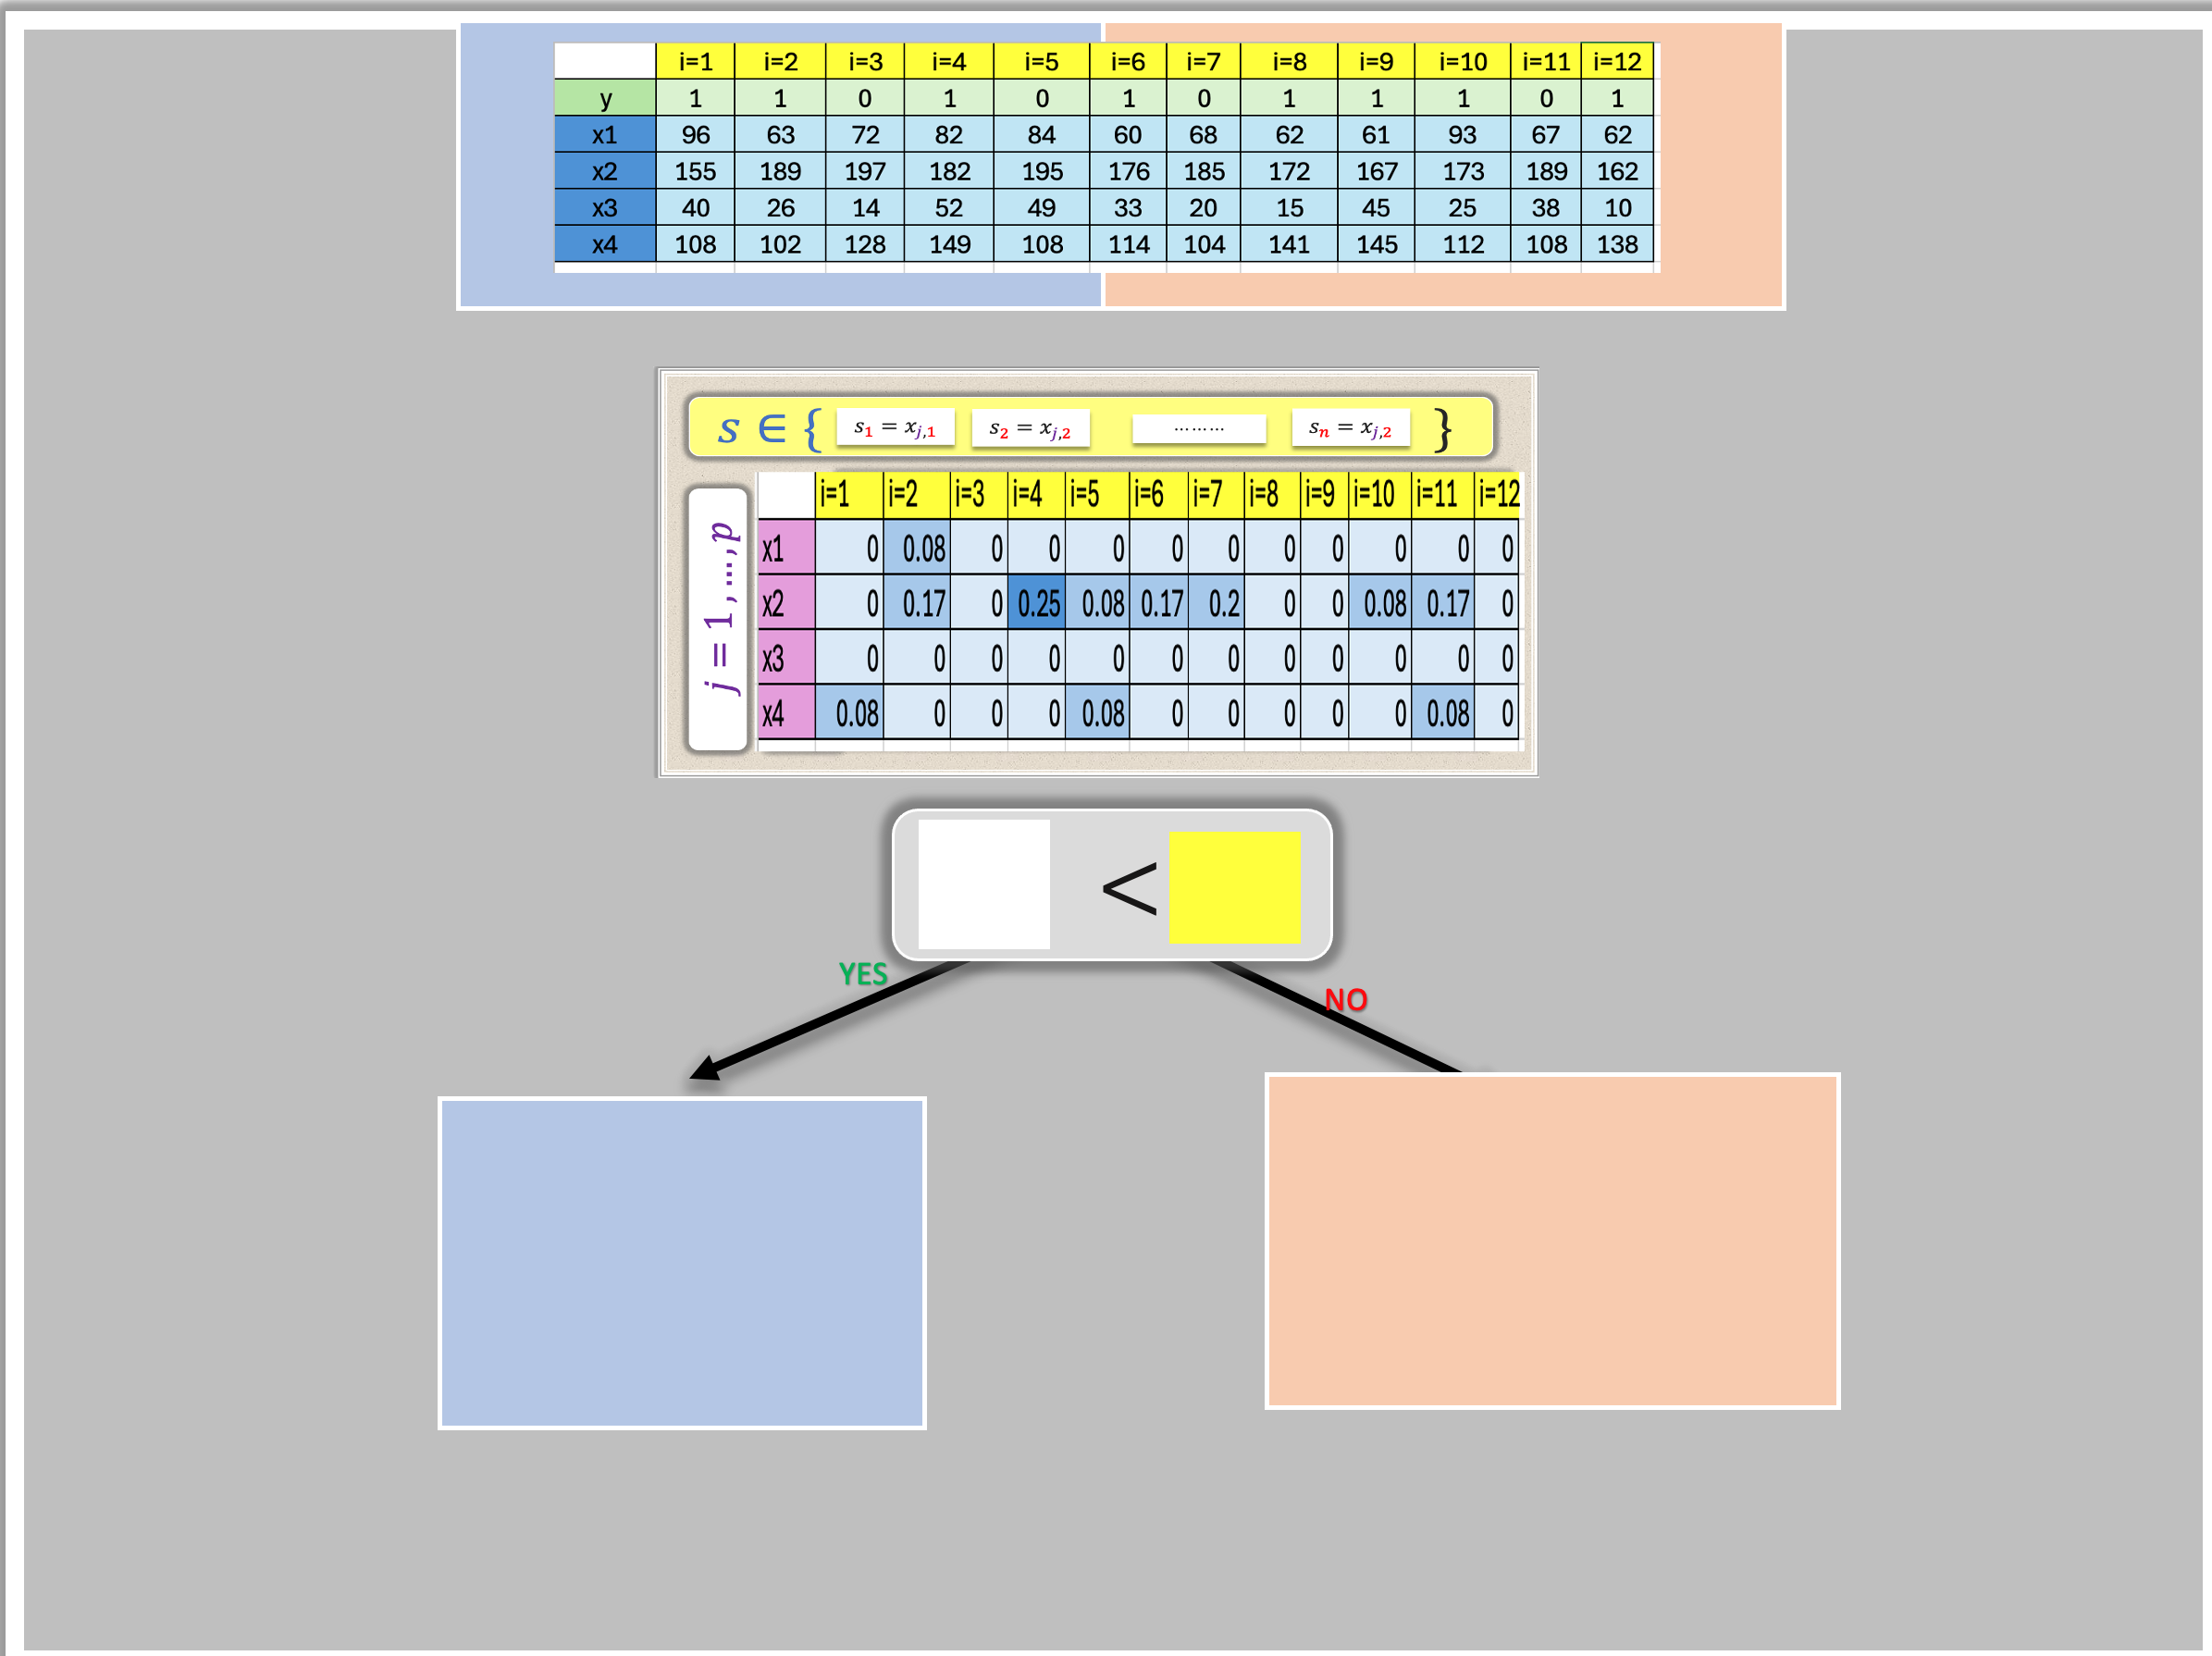
\includegraphics[scale=.28]{figs/1_tree_class.png}
\end{center}
%\vspace{.1in}
%\begin{enumerate}
%\qBrd[4in]{airforceblue!50}{
%\item[\sqBullet{bluebell}] A
%}
%\qBrd[4in]{babyblue!50}{
%\item[\sqBullet{babyblue}]  A
%}
%\end{enumerate}
}\\
\vspace{.8in}

\end{frame}





\begin{frame}
\qBrd[4.7in]{babyblueeyes!50}{
\begin{center}
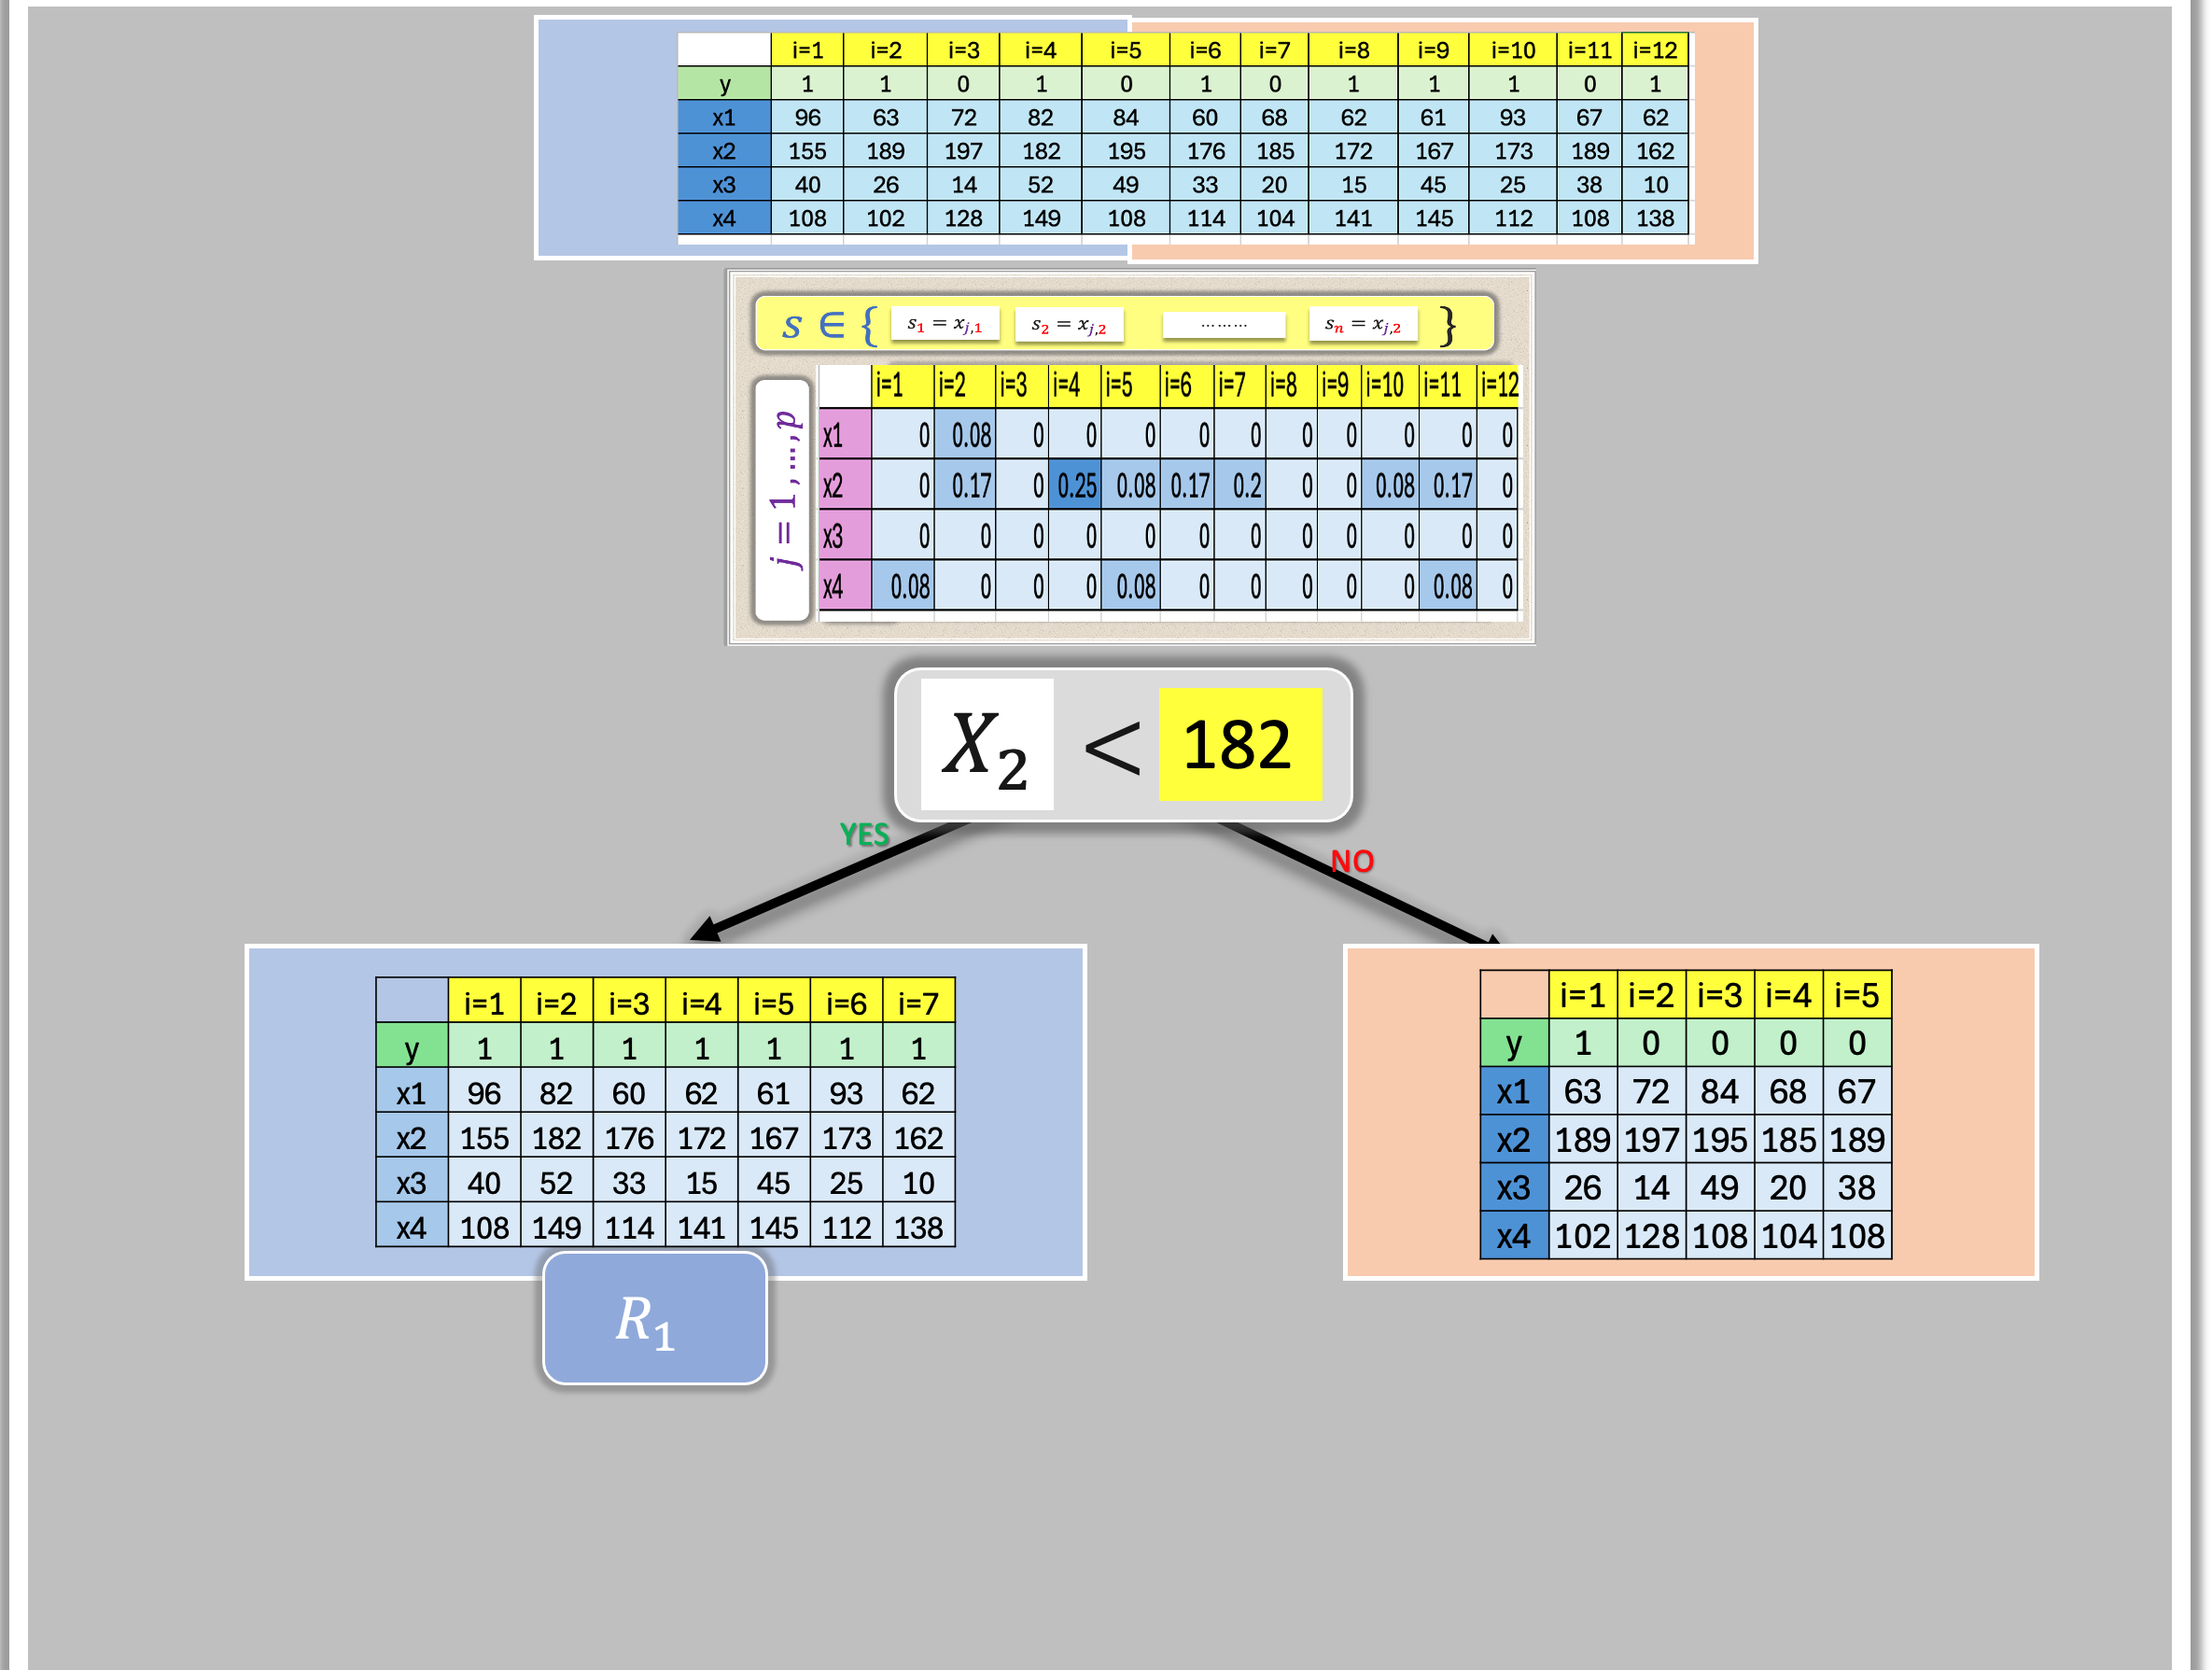
\includegraphics[scale=.28]{figs/2_tree_class.png}
\end{center}
}\\
\vspace{.2in}

\end{frame}




\begin{frame}
\qBrd[4.7in]{babyblueeyes!50}{
\begin{center}
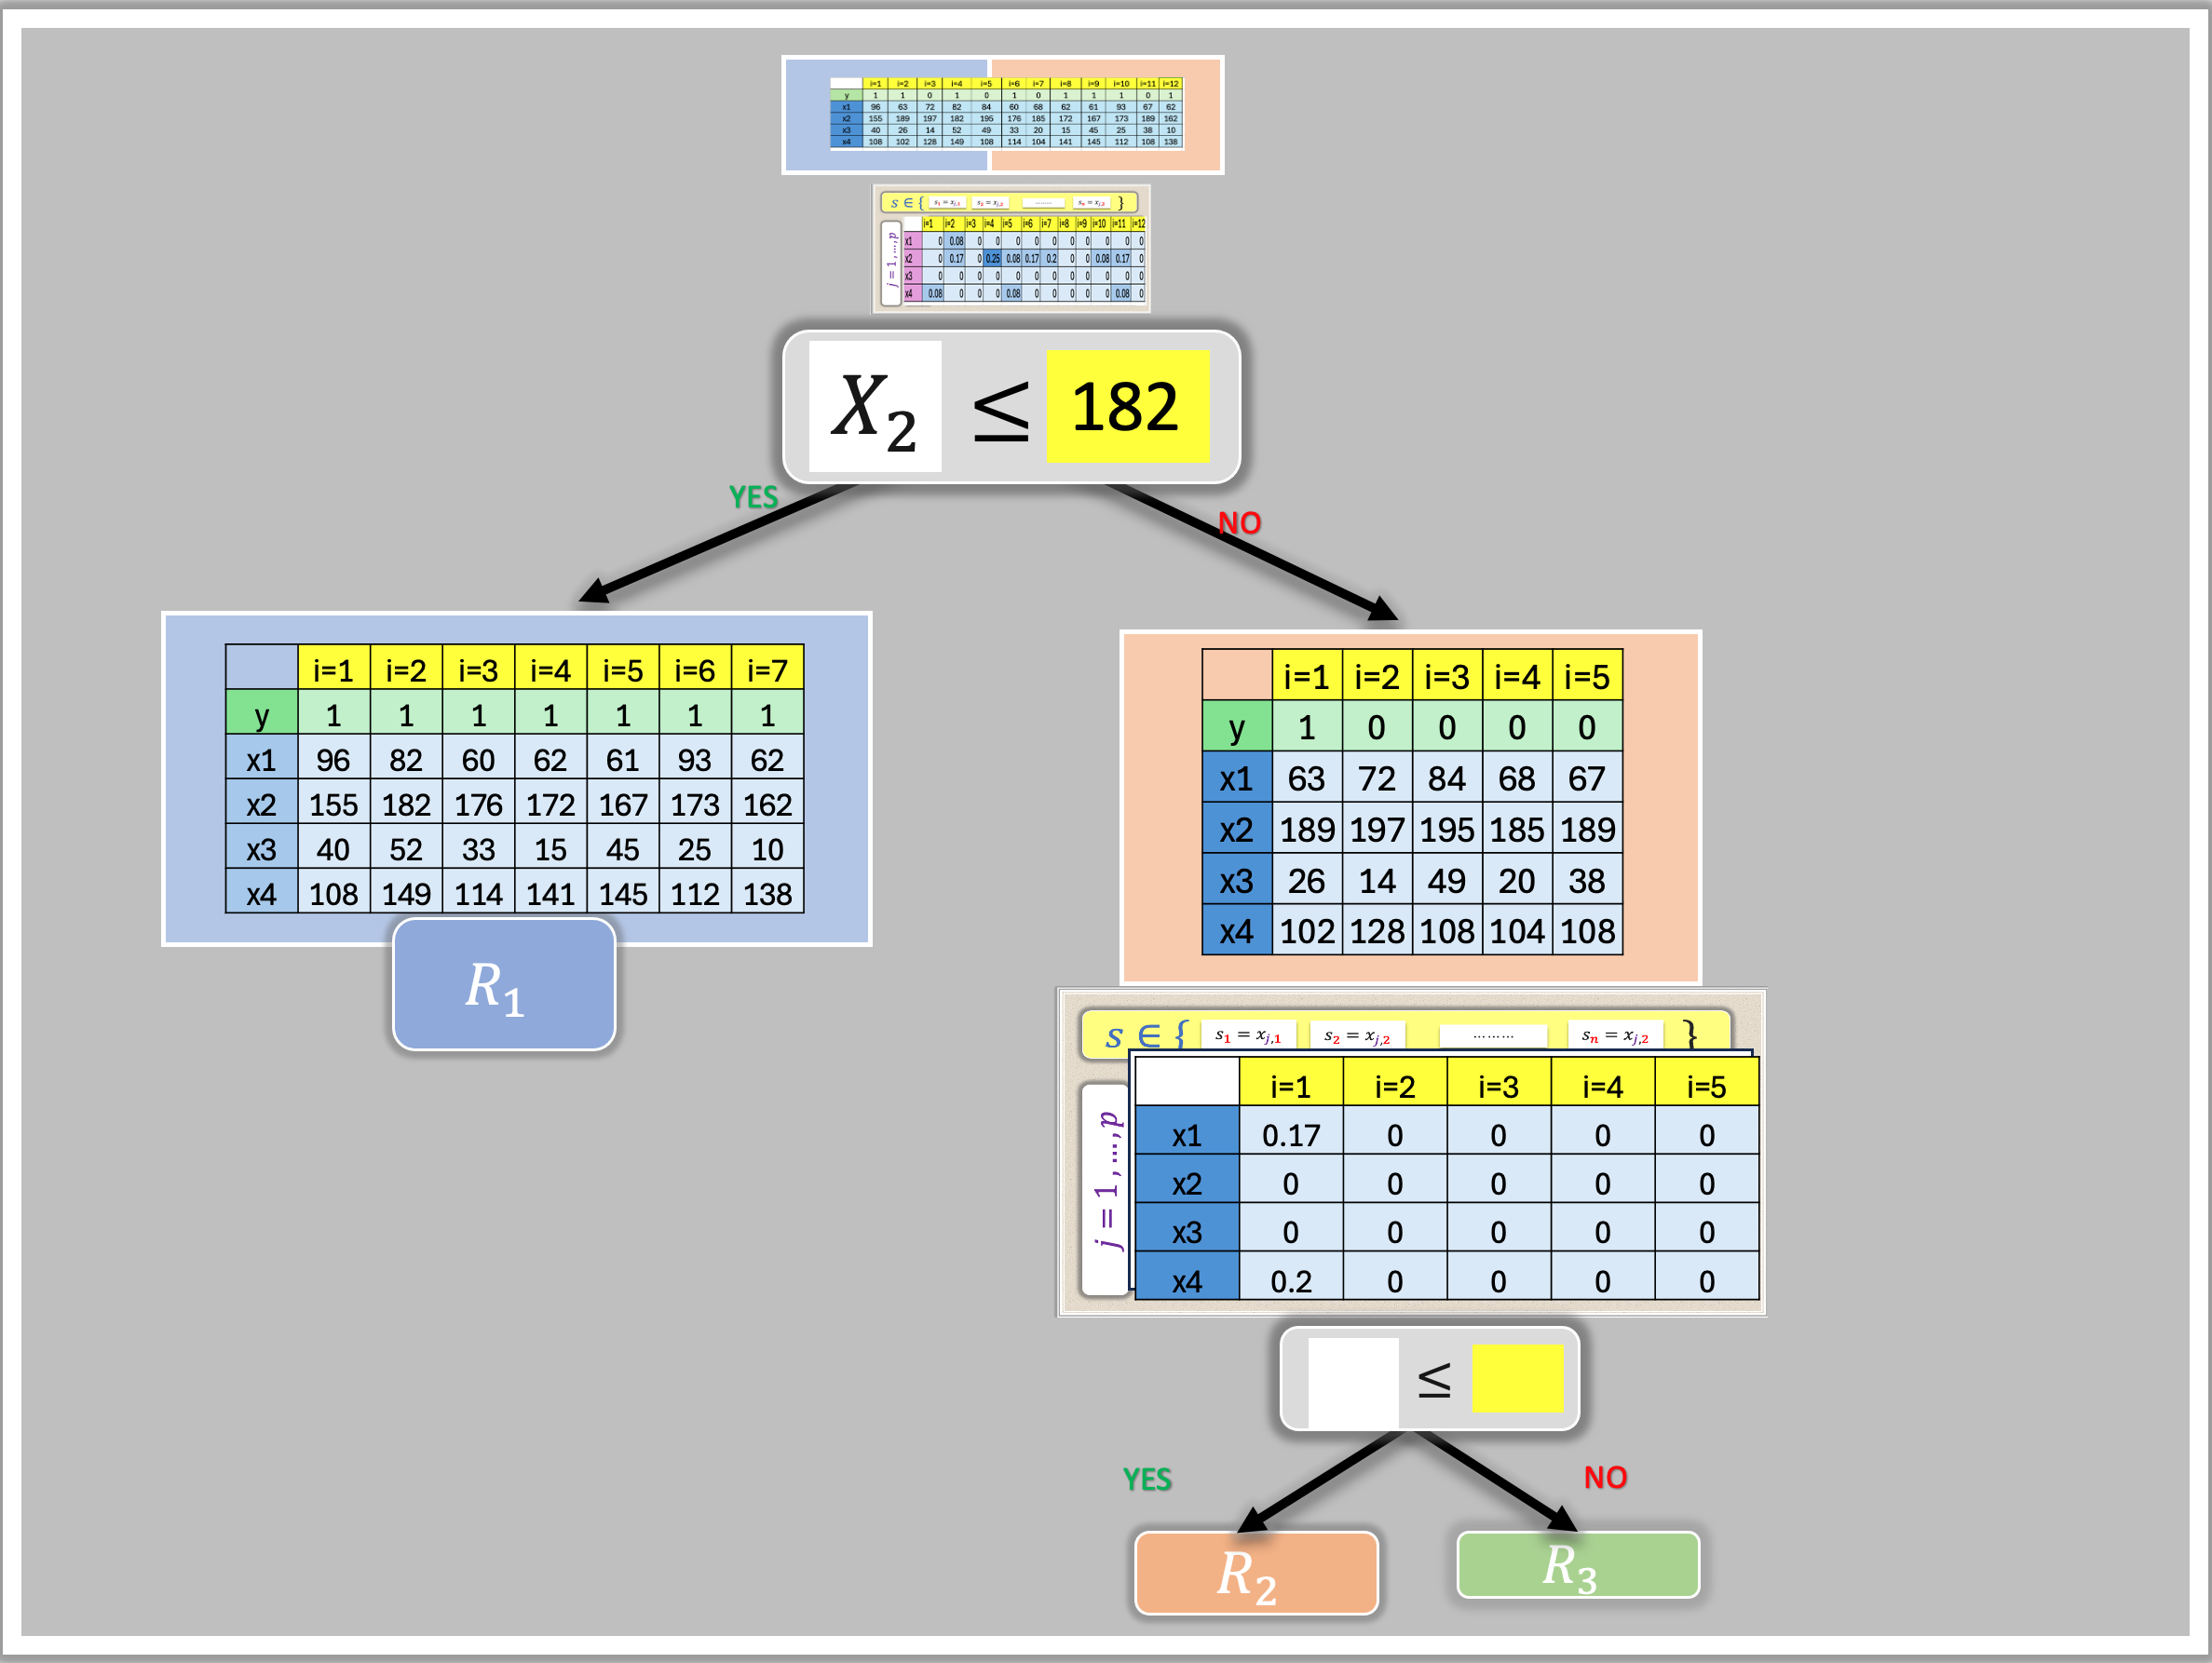
\includegraphics[scale=.25]{figs/3_tree_class.png}
\end{center}
}\\
\vspace{.2in}

\end{frame}



\begin{frame}
\qBrd[4.7in]{babyblueeyes!50}{
\begin{center}
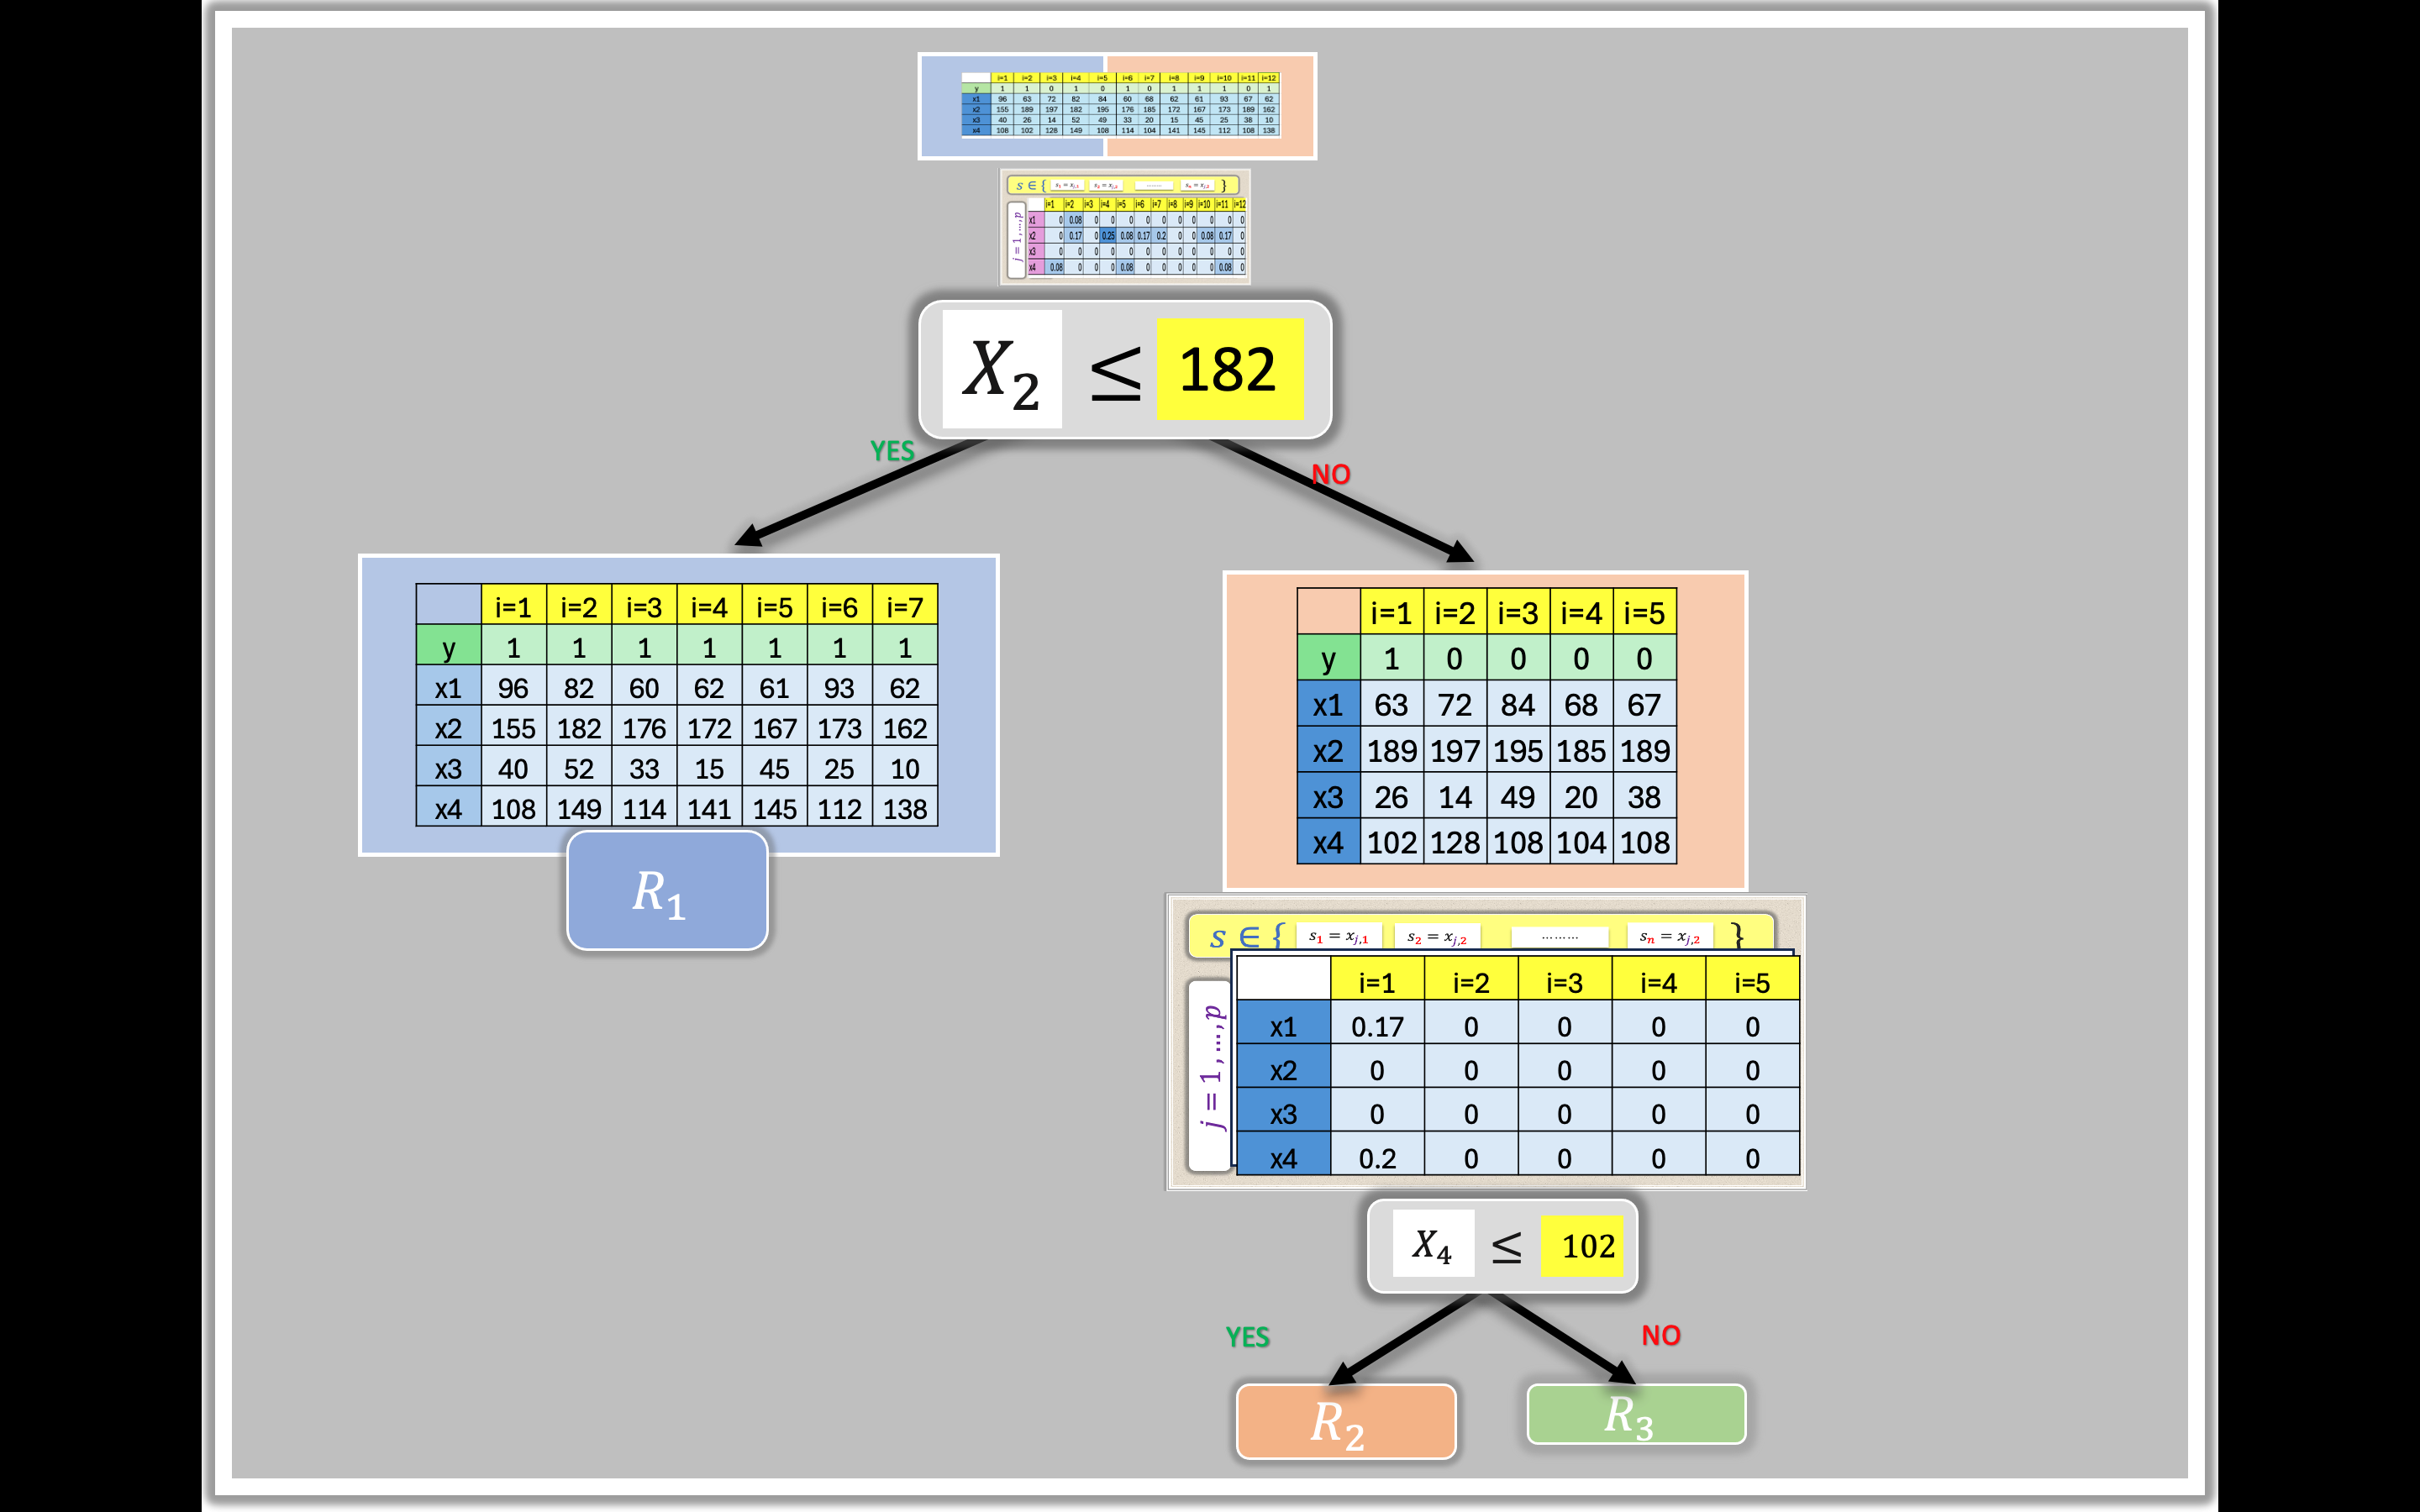
\includegraphics[scale=.25]{figs/4_tree_class.png}
\end{center}
}\\
\vspace{.2in}

\end{frame}



{
 \setbeamercolor{background canvas}{bg=}
%
\includepdf[pages={1}, scale=1, trim=1mm 5mm 11mm 5mm]{STAT380-Unit2.pdf}
\includepdf[pages={97-101}, scale=1]{STAT380-Unit3.pdf}
}


\TransitionFrame[antiquebrass]{\Large Thank You }

\end{document}
